%<dscrpt>Fichier de déclarations Latex à inclure au début des notes de lecture.</dscrpt>

\documentclass[a4paper]{book}
\usepackage[hmargin={1.8cm,1.8cm},vmargin={2.4cm,2.4cm},headheight=13.1pt]{geometry}

%includeheadfoot,scale=1.1,centering,hoffset=-0.5cm,
\usepackage[pdftex]{graphicx,color}

\usepackage[french]{babel}
%\selectlanguage{french}
\addto\captionsfrench{
  \def\contentsname{Plan}
}
\usepackage{fancyhdr}
\usepackage{floatflt}
\usepackage{amsmath}
\usepackage{amssymb}
\usepackage{amsthm}
\usepackage{stmaryrd}

\usepackage[utf8]{inputenc}
\usepackage[T1]{fontenc}

\usepackage[style=numeric,backend=biber]{biblatex}
\usepackage{csquotes}
\addbibresource{NotesKonig.bib}

\usepackage{imakeidx}
\indexsetup{level=\caption,toclevel=section}
\makeindex[title=Index alphabétique]

\usepackage{titletoc}
\dottedcontents{section}[2.5em]{}{1.8em}{1pc}
\dottedcontents{subsection}[3.5em]{}{1.2em}{1pc}
\dottedcontents{subsubsection}[5em]{}{1em}{1pc}

\usepackage[pdftex,colorlinks={true},urlcolor={blue},pdfauthor={remy Nicolai},bookmarks={true}]{hyperref}

\usepackage{multicol}
\usepackage{multirow}
\usepackage{wrapfig}
\usepackage{array}
\usepackage{subfig}

%pr{\'e}sentation du compteur de niveau 2 dans les listes
\makeatletter
\renewcommand{\labelenumii}{\theenumii.}
\renewcommand{\thesection}{\Roman{section}.}
\renewcommand{\thesubsection}{\arabic{subsection}.}
\renewcommand{\thesubsubsection}{\arabic{subsubsection}.}
\makeatother


%dimension des pages, en-t{\^e}te et bas de page
%\pdfpagewidth=20cm
%\pdfpageheight=14cm
%   \setlength{\oddsidemargin}{-2cm}
%   \setlength{\voffset}{-1.5cm}
%   \setlength{\textheight}{12cm}
%   \setlength{\textwidth}{25.2cm}
   \columnsep=1cm
   \columnseprule=0.5pt

%En tete et pied de page
\pagestyle{fancy}
%\lhead{MPSI-\'Eléments de cours}
%\rhead{\today}
%\rhead{25/11/05}
\lfoot{\tiny{Cette création est mise à disposition selon le Contrat\\ Paternité-Pas d'utilisations commerciale-Partage des Conditions Initiales à l'Identique 2.0 France\\ disponible en ligne http://creativecommons.org/licenses/by-nc-sa/2.0/fr/
} }
\rfoot{\tiny{Rémy Nicolai \jobname}}


%\newcommand{\baseurl}{http://back.maquisdoc.net/data/cours\_nicolair/}
%\newcommand{\urlexo}{http://back.maquisdoc.net/data/exos_nicolair/}
\newcommand{\urlcours}{https://maquisdoc-math.fra1.digitaloceanspaces.com/}

\newcommand{\N}{\mathbb{N}}
\newcommand{\Z}{\mathbb{Z}}
\newcommand{\C}{\mathbb{C}}
\newcommand{\R}{\mathbb{R}}
\newcommand{\D}{\mathbb{D}}
\newcommand{\K}{\mathbf{K}}
\newcommand{\Q}{\mathbb{Q}}
\newcommand{\F}{\mathbf{F}}
\newcommand{\U}{\mathbb{U}}
\newcommand{\V}{\mathbb{V}}
\newcommand{\p}{\mathbb{P}}

\newcommand{\ord}{\mathop{\mathrm{ord}}}
\newcommand{\card}{\mathop{\mathrm{Card}}}
\newcommand{\Id}{\mathop{\mathrm{Id}}}
\newcommand{\Ker}{\mathop{\mathrm{Ker}}}
\newcommand{\Vect}{\mathop{\mathrm{Vect}}}
\newcommand{\cotg}{\mathop{\mathrm{cotan}}}
\newcommand{\sh}{\mathop{\mathrm{sh}}}
\newcommand{\ch}{\mathop{\mathrm{ch}}}
\newcommand{\argsh}{\mathop{\mathrm{argsh}}}
\newcommand{\argch}{\mathop{\mathrm{argch}}}
\newcommand{\tr}{\mathop{\mathrm{tr}}}
\newcommand{\rg}{\mathop{\mathrm{rg}}}
\newcommand{\rang}{\mathop{\mathrm{rg}}}
\newcommand{\Mat}{\mathop{\mathrm{Mat}}}
\newcommand{\MatB}[2]{\mathop{\mathrm{Mat}}_{\mathcal{#1}}\left( #2\right) }
\newcommand{\MatBB}[3]{\mathop{\mathrm{Mat}}_{\mathcal{#1} \mathcal{#2}}\left( #3\right) }
\renewcommand{\Re}{\mathop{\mathrm{Re}}}
\renewcommand{\Im}{\mathop{\mathrm{Im}}}
\renewcommand{\th}{\mathop{\mathrm{th}}}
\newcommand{\repere}{$(O,\overrightarrow{i},\overrightarrow{j},\overrightarrow{k})$}
\newcommand{\cov}{\mathop{\mathrm{Cov}}}

\newcommand{\absolue}[1]{\left| #1 \right|}
\newcommand{\fonc}[5]{#1 : \begin{cases}#2 \rightarrow #3 \\ #4 \mapsto #5 \end{cases}}
\newcommand{\depar}[2]{\dfrac{\partial #1}{\partial #2}}
\newcommand{\norme}[1]{\left\| #1 \right\|}
\newcommand{\se}{\geq}
\newcommand{\ie}{\leq}
\newcommand{\trans}{\mathstrut^t\!}
\newcommand{\val}{\mathop{\mathrm{val}}}
\newcommand{\grad}{\mathop{\overrightarrow{\mathrm{grad}}}}

\newtheorem*{thm}{Théorème}
\newtheorem{thmn}{Théorème}
\newtheorem*{prop}{Proposition}
\newtheorem{propn}{Proposition}
\newtheorem*{pa}{Présentation axiomatique}
\newtheorem*{propdef}{Proposition - Définition}
\newtheorem*{lem}{Lemme}
\newtheorem{lemn}{Lemme}

\theoremstyle{definition}
\newtheorem*{defi}{Définition}
\newtheorem{defin}{Définition}
\newtheorem*{nota}{Notation}
\newtheorem*{exple}{Exemple}
\newtheorem{explen}{Exemple}
\newtheorem*{exples}{Exemples}


\newenvironment{demo}{\renewcommand{\proofname}{Preuve}\begin{proof}}{\end{proof}}
%\renewcommand{\proofname}{Preuve} doit etre après le begin{document} pour fonctionner

\theoremstyle{remark}
\newtheorem*{rem}{Remarque}
\newtheorem*{rems}{Remarques}

\renewcommand{\indexspace}{}
\renewenvironment{theindex}
  {\section*{Index} %\addcontentsline{toc}{section}{\protect\numberline{0.}{Index}}
   \begin{multicols}{2}
    \begin{itemize}}
  {\end{itemize} \end{multicols}}

\nocite{*}

\title{
         Notes sur \emph{Measure and Integration} de H. König \\
         \large Rédaction incomplète. Version  beta 3.7
      }
\author{Rémy Nicolaï}

\begin{document}
\maketitle
\tableofcontents
\clearpage

\chapter{Présentation}
\noindent Le livre \emph{Measure and Integration} de Heinz König \cite{könig1997measure} présente des méthodes et des résultats utilisés dans la théorie des mesures. Il se place dans un cadre si général et nécessite une telle érudition que j'ai eu beaucoup de difficultés à le comprendre. Pour m'y aider, j'ai commencé à rédiger des notes de lecture qui détaillent des exemples et reformulent les propriétés et les constructions dans un cadre moins abstrait.\newline
En fait mes difficultés viennent surtout de ma formation qui s'est limitée grosso modo à la préparation à l'agrégation de mathématiques sans probabilités mais avec de la géométrie différentielle (symplectique) et à la lecture assidue des \emph{Éléments d'analyse} de J. Dieudonné (tomes I \cite{dieudonne1969elements} et II \cite{dieudonne1969elements2}).\newline
L'intégration ne se limite pas aux formes linéaires avec de bonnes propriétés sur de bons espaces de fonctions (ou de formes différentielles). Je le savais un peu mais je le sais mieux. Les fonctions avec de bonnes propriétés définies dans des ensembles de parties avec de bonnes propriétés sont un autre versant de la même montagne. Elles interviennent évidemment en probabilité mais aussi dans l'intégration.\newline
Quand on passe de l'intégrale de Riemann à celle de Lebesgue, on passe de fonctions constantes sur des intervalles à des fonctions prenant un nombre fini de valeurs. Pour définir un intégrale, il faut bien attacher une valeur numérique à l'ensemble des points où la fonction prend une valeur donnée.


L'exemple principal est la mesure de Lebesgue dans $\R^n$. Elle vient d'une notion élémentaire de volume pour des hypercubes. Ce volume est étendu d'abord à l'ensemble des parties compactes puis à d'autres ensembles de parties de $\R^n$.\newline
En parallèle, une notion de densité arithmétique formée à partir de classes de congruence tente d'introduire une probabilité dans $\Z$. L'échec de cette tentative répond à l'échec de l'extension du volume à l'ensemble des parties seulement fermées. Ce parallelisme donne du relief aux développements du livre et appelle à éclaircir le rôle de la compacité.

\paragraph*{Systèmes et fonctions d'ensembles.}
Les objets fondamentaux utilisés dans la théorie des mesures sur un ensemble $X$ sont des parties $\mathfrak{S}$ de $\mathcal{P}(X)$ (appelés \emph{pavings} dans le livre) et des fonctions $\varphi$ définies dans $\mathfrak{S}$ à valeurs dans $\overline{\R}$ (appelés \emph{set fonctions} dans le livre).\newline
Avec le sens précis que prend le mot \emph{pavage} dans les mathématiques en France, on ne peut traduire \emph{paving} par \emph{pavage}. Comme l'auteur utilise aussi \emph{set system}, j'utiliserai \emph{système d'ensembles} pour désigner un \emph{paving} c'est à dire simplement une partie de $\mathcal{P}(X)$.\newline
Une fonction de $\mathfrak{S}$ dans $\overline{\R}$ sera désignée par \emph{fonction d'ensembles} (\emph{set fonction} dans le texte).

\begin{enumerate}
 \item  Les différents types de systèmes d'ensembles sont présentés en \ref{Chap:SystFoncEns}\ref{Sec:SystEns} et définis à partir des stabilités relativement aux opérations ensemblistes union, intersection, soustraction ensembliste, complémentation.\newline
 En particulier un système d'ensembles est un \emph{treillis} (lattice) si et seulement si il est stable pour l'union et l'intersection.
 \item Les propriétés significatives des fonctions d'ensembles sont présentées dans le chapitre \ref{Chap:SystFoncEns} section \ref{Sec:FoncEns}. Les plus fondamentales pour une fonction définie dans un treillis sont l'isotonie (croissance) et la modularité (sorte d'additivité).
 \begin{displaymath}
   \begin{aligned}
     \forall (A,B) \in \mathfrak{S}^2, \;& A \subset B \Rightarrow \varphi(A) \leq \varphi(B) &\text{isotonie}& \\
     \forall (A,B) \in \mathfrak{S}^2, \;&  \varphi(A\cap B) + \varphi(A \cup B) = \varphi(A) + \varphi(B) &\text{modularité}&
   \end{aligned}
 \end{displaymath}

 \item Les concepts proches des mesures (chapitre \ref{Chap:SystFoncEns} section \ref{Sec:FoncEns} \ref{SubSec:ContenusMesures} ) sont des cas particuliers des situations précédentes.
 \item À partir d'une fonction d'ensembles $\varphi$, on peut construire (\ref{Chap:ExtenRegul} \ref{Sec:Enveloppes}) une fonction d'ensemble $\Phi$ définie dans $\mathcal{P}(X)$ tout entier qui possède de bonnes propriétés.
 \item La classe de Carathéodory (chap \ref{Chap:ExtenRegul} section \ref{Sec:ClasseCaratheodory}) d'une fonction d'ensemble sur $\mathcal{P}(X)$ est un système d'ensembles qui possède de bonnes propriétés. C'est le cadre de la preuve de résultats importants.
\end{enumerate}

On notera $A'$ le complémentaire d'une partie $A \in \mathcal{P}(X)$ pour un ensemble $X$ quelconque.
\newpage

\chapter{Exemples}\label{Chap:Exples}
Deux exemples sont présentés. À côté du volume dans $\R^n$ qui est l'exemple principal du livre, je présente une fonction d'ensembles sur les parties de $\Z$ définie par des procédés analogues. Pour le moment, je nomme \emph{densité arithmétique} cette fonction d'ensembles. Les deux constructions sont parallèles.

\section{Cellules de base}\label{Sec:CellulesBases}

\subsection{Cubes rationnels}\label{SubSec:CubesRat}
Dans cet exemple qui est l'exemple fondamental du livre, $X=\R^n$. Dans tout le livre, on pourra utiliser occasionnellement la \emph{norme infinie} de $\R^n$ ainsi qu'un résultat sur les intervalles. \index{norme infinie de $\R^n$}
\begin{defi}[Norme infinie de $\R^n$]
 On note $N$ la norme infinie de $\R^n$ définie par
 \begin{displaymath}
  \forall x=(x_1,\cdots,x_n)\in X= \R^n, \; N(x)=\max(|x_1|,\cdots,|x_n|).
 \end{displaymath}
\end{defi}

 \paragraph{Exercice sur des intervalles} \label{ExoIntervalles}
 Soit $x\leq y$ et $a\leq b$ réels. Montrer que
 \begin{displaymath}
  [x,y] \cap [a,b] \neq \emptyset
  \Leftrightarrow
  \left\lbrace
  \begin{aligned}
    x \leq b \\
    a \leq y
  \end{aligned}
  \right.
  \Leftrightarrow \max(x,a)\leq \min(y,b).
 \end{displaymath}
 Dans ce cas $[x,y]\cap [a,b] = [\max(x,a),\min(y,b)]$.
\begin{demo}
Pour tout réel $u$,
\begin{displaymath}
 u \in [x,y] \cap [a,b]
 \Leftrightarrow
 \left\lbrace
 \begin{aligned}
   x \leq u \leq y \\
   a \leq u \leq b
 \end{aligned}
 \right.
 \Leftrightarrow
   \max(x,a) \leq u \leq \min(y,b) .
 \end{displaymath}
\end{demo}

\begin{defi}[q-cube]\index{q-cube}\label{q-cube}
Pour tout naturel non nul $q$, on appelle $q$-cube un hypercube fermé de côté $\frac{1}{q}$ et de sommets à coordonnées dans $\frac{1}{q}\Z^n$.\newline
Par exemple, pour $a = (a_1, \cdots, a_n) \in \frac{1}{q}\Z^n$, on définit le $q$-cube $Q_a$ par
\begin{displaymath}
 \forall x = (x_1, \cdots, x_n) \in X, \; x \in Q_a  \Leftrightarrow \forall i \in \llbracket 1,n \rrbracket,\; a_i \leq x_i \leq a_i + \frac{1}{q}.
\end{displaymath}
On peut voir aussi $Q_a$ comme un produit cartésien de segments
\begin{displaymath}
 Q_a = [a_1, a_1+\frac{1}{p}] \times \cdots \times [a_n, a_n+\frac{1}{p}].
\end{displaymath}
On note $\mathfrak{C}_q$ l'ensemble des $q$-cubes. On dit aussi cube de taille $\frac{1}{q}$ plutôt que $q$-cube.
\end{defi}
\begin{rems}
 \begin{itemize}
  \item Un $1$-cube est un cube de côté $1$ et de sommets à coordonnées entières.
  \item Pour tout $q$-cube $Q$, il existe un unique $a\in \frac{1}{q}\Z^n$ tel que $Q=Q_a$.
  \item Les $q$-cubes recouvrent $X$. Plus précisément
  \begin{displaymath}
     X = \R^n = \bigcup_{a\in \frac{1}{q}\Z}Q_a = \bigcup_{Q\in \mathfrak{C}_q}Q.
  \end{displaymath}
  \item L'intersection de 2 cubes distincts qui se coupent n'est pas un $q$-cube. Par exemple en dimension $n=3$ c'est une face, une arête ou un sommet. Pour rendre compte de ces intersections, on introduit la notion de cellule.
 \end{itemize}
\end{rems}

\index{cellule de taille $\frac{1}{q}$ et de dimension $d$}
\begin{defi}[q-d-cellule]
 Pour $a = (a_1, \cdots, a_n) \in \frac{1}{q}\Z^n$ et $I$ une partie à $d$ éléments de $\llbracket 1,n \rrbracket$, on définit la $q$-$d$-cellule $C_a(I)$ par
\begin{displaymath}
 \forall x = (x_1, \cdots, x_n) \in X, \; x \in C_a(I)  \Leftrightarrow
 \left\lbrace
   \begin{aligned}
      &\forall i \in I,&\; a_i \leq x_i \leq a_i + \frac{1}{q} \\
      &\forall i \in \llbracket 1,n \rrbracket \setminus I, &\; x_i = a_i
   \end{aligned}
  \right. .
\end{displaymath}
\end{defi}
\begin{rem}
On dira aussi cellule de taille $\frac{1}{q}$ et de dimension $d$ plutôt que $q$-$d$-cellule.\newline
Dans $X=\R^n$, un $q$-cube est une cellule de taille $\frac{1}{q}$ et de dimension $n$. Une de ses arêtes est une cellule de dimension 1 (taille $\frac{1}{q}$). Une face est une cellule de dimension $n-1$. Un singleton dans $\frac{1}{p} \Z^n$ est une cellule de taille $\frac{1}{q}$ et de dimension nulle.
\end{rem}
\begin{propn}
 Lorsque deux cellules de taille $\frac{1}{q}$ distinctes ne sont pas disjointes, leur intersection est une cellule de taille $\frac{1}{q}$.
\end{propn}
\begin{demo}
 Commençons par l'intersection de deux $q$-cubes distincts $Q_a$ et $Q_b$.
 \begin{multline*}
  Q_a \cap Q_b \neq \emptyset
   \Leftrightarrow
  [a_1, a_1+\frac{1}{p}] \times \cdots \times [a_n, a_n+\frac{1}{p}] \cap [b_1, b_1+\frac{1}{p}] \times \cdots \times [b_n, b_n+\frac{1}{p}] \neq \emptyset \\
   \Leftrightarrow
  \forall i \in \llbracket 1,n \rrbracket, \; [a_i, a_i+\frac{1}{p}] \cap [b_i, b_i+\frac{1}{p}] \neq \emptyset
   \Leftrightarrow
  \forall i \in \llbracket 1,n \rrbracket, \; a_i \leq b_i + \frac{1}{q} \text{ et } b_i \leq a_i + \frac{1}{q} \text{ (exercice sur intervalles)} \\
   \Leftrightarrow
  N(b-a) \leq \frac{1}{q}
   \Leftrightarrow
  N(b-a) = \frac{1}{q}
   \Leftrightarrow
  \forall i \in \llbracket 1,n \rrbracket, \; |a_i - b_i| = 0 \text{ ou } \frac{1}{q}.
 \end{multline*}
car $a$ et $b$ appartiennent à $\frac{1}{q}\, \Z^n$. Définissons un $c=(c_1,\cdots,c_n) \in \frac{1}{q}\,\Z^n$ en classant les indices $i$ en trois catégories. Pour tout $i \in \llbracket \rrbracket$:
\begin{align*}
 i \in I & \Leftrightarrow a_i = b_i               &\text{ on pose } c_i = a_i = b_i\\
 i \in J & \Leftrightarrow a_i = b_i + \frac{1}{q} &\text{ on pose } c_i = a_i\\
 i \in K & \Leftrightarrow b_i = a_i + \frac{1}{q} &\text{ on pose } c_i = b_i
\end{align*}
Pour tout $x = (x_1, \cdots, x_n) \in \R^n$:
\begin{displaymath}
 x \in Q_a \cap Q_b \Leftrightarrow
 \left\lbrace
   \begin{aligned}
     &\forall i \in I,&\; a_i \leq x_i \leq a_i + \frac{1}{q} \\
     &\forall i \in J\cup K,&\; x_i = c_i
   \end{aligned}
  \right. .
\end{displaymath}
On en déduit que $Q_a \cap Q_b$ est une cellule de taille $\frac{1}{q}$ et de dimension $\sharp I$.\newline
Considérons maintenant deux cellules $C_a(I)$ et $C_b(J)$.
\begin{displaymath}
 x=(x_1,\cdots,x_n) \in C_a(I) \cap C_b(J)
  \Leftrightarrow
    \left\lbrace
      \begin{aligned}
         &\forall i \in I \cap J,& x_i \in [a_i, a_i+\frac{1}{p}] \cap [b_i, b_i+\frac{1}{p}] \neq \emptyset \\
         &\forall i \in I \setminus J,&  x_i = b_i \in [a_i, a_i+\frac{1}{p}] \\
         &\forall i \in J \setminus I,&  x_i = a_i \in [b_i, b_i+\frac{1}{p}] \\
         &\forall i \in I'\cap J',& x_i = a_i = b_i
      \end{aligned}
    \right.
\end{displaymath}
Pour tous les indices $i$ qui ne sont pas dans $I \cap J$, seule une valeur de $x_i$ est possible. Pour les autres, on est ramené à une intersection de deux cubes dans $\R^d$ avec $d=\sharp I\cap J$.
\end{demo}

\begin{propn}\label{DecompCellule}
 Soit $m=pq$ un multiple de $p$. Toute cellule de taille $\frac{1}{q}$ et de dimension $d$ est une union de cellules de taille $\frac{1}{m}$ et de même dimension (au nombre de $p^d$). En particulier, tout cube de taille $\frac{1}{q}$ est l'union de $p^n$ cubes de taille $\frac{1}{m}$.
\end{propn}
\begin{demo}
En considérant les coordonnées fixées pour une cellule, il suffit de le démontrer pour les cubes.
 Soit $Q = Q_a$ avec $a = (a_1, \cdots, a_n) \in \frac{1}{q}\Z^n$ un $q$-cube quelconque.\newline
 Notons $k=(k_1,\cdots,k_n)\in \llbracket 0, p-1\llbracket^n$ puis $a(k)=(a_1 + \frac{k_1}{m}, \cdots a_n + \frac{k_n}{m})$ et $Q_{a(k)}$ le $m$-cube associé. Alors
 \begin{displaymath}
  Q_a = \bigcup_{k=(k_1,\cdots,k_n)\in \llbracket 0, p-1\llbracket^n}\, Q_{a(k)}.
 \end{displaymath}
\end{demo}

\begin{defi}
  On note $\mathfrak{S}_q$ l'ensemble des unions finies de cellules de taille $\frac{1}{q}$ et $\mathfrak{S} = \bigcup_{q\in \N} \mathfrak{S}_q$.
\end{defi}

\begin{propn}
 Pour tout naturel $q$ non nul, $\mathfrak{S}_q$ est stable pour l'union et l'intersection. C'est un treillis.\newline
 Soit $m$ un multiple de $q$. Alors $\mathfrak{S}_q \subset \mathfrak{S}_m$.
\end{propn}
\begin{demo}
 Conséquence des deux propositions précédentes.
\end{demo}

\noindent On définit le volume dans $\mathfrak{S}$ à partir du cube unité et de son unique décomposition, de l'invariance par translation, de la modularité.
\begin{itemize}
 \item Le volume du cube unité dans $\mathfrak{S}_0$ est 1.
 \item Toute cellule de dimension strictement plus petite que $n$ est de volume nul
 \item Par translation, tous les cubes de taille $\frac{1}{q}$ ont le même volume.
 \item Le cube unité se décompose de manière unique en $q^{n}$ cubes dans $\mathfrak{S}_q$. Par modularité, le volume d'un cube de taille $\frac{1}{q}$ est $\frac{1}{q^{n}}$.
\end{itemize}

\begin{defi}[volume dans l'ensemble des unions finies de cellules]\label{DefVolUnionCell}
Soit $A \in \mathfrak{S}$, il existe $s\in \N$ et un ensemble fini $\mathfrak{A}$ de cellules de taille $\frac{1}{q}$ tels que $A = \bigcup_{Q\in \mathfrak{A}} Q$. On désigne par $\mathfrak{A}_n \subset \mathfrak{A}$ l'ensemble des cubes. On définit le volume $\lambda(A)$ par
\begin{displaymath}
 \lambda(A) = \frac{\sharp \mathfrak{A}_n}{q^{n}}.
\end{displaymath}
\end{defi}
\begin{demo}[Consistence de la définition]
 Si $A$ se décompose en une union de cellules de taille $\frac{1}{q}$ et en une union de cellules de taille $\frac{1}{r}$, les deux valeurs du volume de $A$ sont-elles égales?\newline
 Considérons un multiple commun $m=pq$. D'après la proposition \ref{DecompCellule}, $A$ est une union de cellules de taille $\frac{1}{m}$. Il suffit de montrer que le volume est le même pour $q$ et $m$.\newline
 Notons $\mathfrak{B}_n$ l'ensemble fini des cubes de taille $\frac{1}{m}$ dans la décomposition de $A$ (les cellules de dimension plus petites ne comptent pas pour le volume). D'après la proposition \ref{DecompCellule}, $\sharp \mathfrak{B}_n = p^n \times \sharp \mathfrak{A}_n$. On en déduit
 \begin{displaymath}
  \frac{\sharp \mathfrak{B}_n}{m^{n}} = \frac{p^n \times \sharp \mathfrak{A}_n}{p^n \times q^{n}} = \frac{\sharp \mathfrak{A}_n}{q^{n}} = \lambda(A).
 \end{displaymath}
\end{demo}
\begin{rem}
 Lorsque $A$ est une union finie de cellules de taille $\frac{1}{q}$, son volume est le nombre de cubes de taille $\frac{1}{q}$ \emph{inclus dans } $A$ multiplié par $\frac{1}{q}$.
\end{rem}
\begin{propn}
 La fonction d'ensembles $\lambda$ (volume) définie dans le treillis $\mathfrak{S}$ des unions finies de cellules à valeurs dans $[0,+\infty[$ est isotone (croissante) et modulaire.
\end{propn}
\begin{demo}
 Soit $A$ et $B$ deux unions de cellules de taille $\frac{1}{q}$. Notons $\mathfrak{A}$, $\mathfrak{B}$, $\mathfrak{U}$, $\mathfrak{I}$ les ensembles de cubes que contiennent respectivement $A$, $B$, $A\cup B$, $A\cap B$.
 \begin{align*}
  A \subset B \Rightarrow \mathfrak{A} \subset \mathfrak{B} \Rightarrow \sharp\mathfrak{A} \leq \sharp \mathfrak{B} \Rightarrow& \varphi(A) \leq \varphi(B) \\
  \mathfrak{A}\cup \mathfrak{B} = \mathfrak{U} \Rightarrow& \varphi(A\cup B) = \frac{\sharp(\mathfrak{A}\cup \mathfrak{B})}{q^n} \\
  \mathfrak{A}\cap \mathfrak{B} = \mathfrak{I} \Rightarrow& \varphi(A\cap B) = \frac{\sharp(\mathfrak{A}\cap \mathfrak{B})}{q^n}
 \end{align*}
 en multipliant par $\frac{1}{q^n}$. On conclut avec la modularité de la fonction nombre d'éléments
 \begin{displaymath}
  \sharp(\mathfrak{A}\cup \mathfrak{B})) + \sharp(\mathfrak{A}\cap \mathfrak{B})) = \sharp\mathfrak{A} + \sharp \mathfrak{B}.
 \end{displaymath}
\end{demo}

\subsection{Classes de congruences entières}\label{SubSec:ClassesCongru}
Ici $X = \Z$. \index{Exemple arithmétique}
L'ensemble des unions finies de classes de congruence défini au dessous sera désigné dans tout le document par \og~ Exemple arithmétique~\fg{}.

\begin{defi}
On désigne par $\mathfrak{C}_m \subset \mathcal{P}(\Z)$ l'ensemble des classes de congruences modulo un naturel non nul $m$, par $\mathfrak{S}_m$ l'ensemble des unions de classes modulo $m$, par $\mathfrak{C} = \bigcup_{m \in \N^*}\mathfrak{C}_m$ l'ensemble des classes de congruences et par $\mathfrak{S}$ l'ensemble des unions finies d'éléments de $\mathfrak{C}$.
\end{defi}
\begin{rems}
 \begin{itemize}
  \item Soit $A \subset \Z$,
  \begin{align*}
 A \in \mathfrak{C}  &\Leftrightarrow \exists m\in \N^*,\, \exists a \in \llbracket 0, m \llbracket \text{ tq } A = a + \Z m \\
 A\in \mathfrak{S} &\Leftrightarrow \exists (m_1,\cdots,m_p) \in (\N^*)^p, \exists (a_1,\cdots,a_p)\in \llbracket 0,m_1\llbracket \times \dots \times \llbracket 0,m_p\llbracket \text{ tq }\;
 A = \bigcup_{i=1}^{p}(a_i + \Z m_i)
  \end{align*}
    \item Les ensembles $\mathfrak{C}_m$ et $\mathfrak{S}_m$ sont finis avec $\sharp \mathfrak{C}_m = m, \; \sharp \mathfrak{S}_m = 2^m$.
  \end{itemize}
\end{rems}

\begin{propn} \label{décompoClasse}
 Soit $m\in \N^*$ diviseur de $p\in \N^*$ avec $p=qm$.\newline
 Pour tout $a\in \Z$, $a + p\Z \subset a + m\Z$. Chaque classe modulo $m$ se décompose en $q$ classes modulo $p$.
 \begin{displaymath}
  \left( \forall A\in \mathfrak{C}_m, \;  A = \bigcup_{C \in \mathfrak{C}_p,\, C\subset A} C \right) \Rightarrow \mathfrak{C}_m \subset \mathfrak{S}_p.
 \end{displaymath}
\end{propn}
\begin{demo}
 $a + p \Z = a + qm\Z \subset a + m\Z$. Pour tout $x \in  a + m\Z = A \in \mathfrak{C}_m$, il existe $k \in \Z$ tel que $x = a + km$. Divisons $k$ par $q$, il existe $\lambda \in \Z$ et $r \in \llbracket 0, q\llbracket$ tels que
 \begin{displaymath}
  x = a + (r+\lambda q)m = a+rm + \lambda qm \in a+rm + p \Z = C \in \mathfrak{C}_p \text{ avec } C \subset A.
 \end{displaymath}
 On en déduit $A \subset \bigcup_{C \in \mathfrak{C}_p,\, C\subset A} C$, l'autre inclusion est évidente.
\end{demo}
 \label{ExpleZ}
 \noindent On en déduit que pour tout multiple $q$ de $p$, $\mathfrak{C}_p \subset \mathfrak{S}_q$ donc $\mathfrak{S}_p \subset \mathfrak{S}_q$. En utilisant un multiple commun des modulos des classes, on montre que $\mathfrak{S}= \bigcup_{q \in \N^*}\mathfrak{S}_q$. Autrement dit, toute union finie de classes de congruence se décompose en une union finie de classes modulo \emph{le même} naturel non nul.

 \begin{propn} \label{prop:DecompUnionClasses}
  Soit $A=\bigcup_{i=1}^n(a_i + \Z m_i) \in \mathfrak{S}$ et $p$ un multiple commun aux $m_i$.\newline
  Pour tout $C \in \mathfrak{C}p$, $C \cap A \neq \emptyset \Leftrightarrow C \subset A$. De plus,
  \begin{displaymath}
   A = \bigcup_{C \in \mathfrak{C}_p,\, C\subset A} C = \bigcup_{C \in \mathfrak{C}_p,\, C\cap A \neq \emptyset} C.
  \end{displaymath}
 \end{propn}
 \begin{demo}
  Supposons $C\cap A \neq \emptyset$. Il existe $i$ tel que $a_i + \Z m_i$ contienne un $a \in C$ c'est à dire tel que $a \equiv a_i \mod m_i$. Pour tout $x \in C$:
  \begin{displaymath}
   x \equiv a \mod p \Rightarrow x \equiv a \mod m_i \Rightarrow x \equiv a_i \mod m_i \Rightarrow x \in a_i + \Z m_i \subset A.
  \end{displaymath}
  On en déduit $C \cap A \neq \emptyset$ entraine $C \subset A$. La réciproque est évidente.\newline
  La décomposition d'un élément de $\mathfrak{S}$ est une conséquence de la décomposition d'une classe de congruence. Chaque $a_i + \Z m_i$ se décompose en une union de $C\in \mathfrak{C}_p$ tels que $C \subset a_i + \Z m_i \subset A$. On en déduit $A = \bigcup_{i=1}^n(a_i + \Z m_i) \subset \bigcup_{C \in \mathfrak{C}_p,\, C\subset A} C$, l'autre inclusion est évidente.
 \end{demo}

\begin{defi}[densité arithmétique dans l'ensemble des unions de classes de congruence]\label{Def:DensitClassCongr}
 Soit $A \in \mathfrak{S}$. Il existe $p \in \N^*$ et un ensemble fini $\mathfrak{A}$ de classes de congruence tels que $A = \bigcup_{C \in \mathfrak{A}}C$. On définit la densité arithmétique $\varphi(A)$ par:
 \begin{displaymath}
  \varphi(A) = \frac{\sharp \mathfrak{A}}{p}.
 \end{displaymath}
 En convenant que $\varphi(\emptyset) = 0$.
\end{defi}
\begin{demo}[Consistence de la définition]
Supposons que $A$ se décompose en classes modulo $p$ et en classes modulo $p'$. Considérons un multiple commun $q$. Notons respectivement $\mathfrak{A}_p$, $\mathfrak{A}_{p'}$, $\mathfrak{A}_q$ les ensembles de classes modulo respectivement $p$, $p'$, $q$ qui décomposent $A$. D'après la proposition \ref{décompoClasse}:
\begin{displaymath}
\left\lbrace
  \begin{aligned}
     \sharp \mathfrak{A}_q &= \frac{q}{p}  \, \sharp \mathfrak{A}_p \\
     \sharp \mathfrak{A}_q &= \frac{q}{p'} \, \sharp \mathfrak{A}_{p'}
  \end{aligned}
\right. \Rightarrow
\left\lbrace
 \begin{aligned}
    \frac{\sharp \mathfrak{A}_q}{q} &= \frac{\sharp \mathfrak{A}_p}{p} \\
    \frac{\sharp \mathfrak{A}_q}{q} &= \frac{\sharp \mathfrak{A}_p'}{p'}
 \end{aligned}
\right . \Rightarrow \frac{\sharp \mathfrak{A}_p}{p} = \frac{\sharp \mathfrak{A}_p'}{p'}.
\end{displaymath}
\end{demo}

\begin{rems}
 \begin{enumerate}
  \item  Aucun singleton n'est dans $\mathfrak{C}$ car les modulos sont non nuls. En revanche $\Z \in \mathfrak{C} \subset \mathfrak{S}$ car c'est la classe de $0$ modulo $1$.

  \item Par définition, $\mathfrak{S}$ est stable pour $\cup$. Il est aussi stable par complémentation à cause de la proposition \ref{prop:DecompUnionClasses} et de la partition en classes. Soit $A\in \mathfrak{S}$. Il existe $p$ naturel non nul et $\mathfrak{A}\subset \mathfrak{C}_p$ tels que $A = \bigcup_{C \in \mathfrak{A}} C$. Alors $A' = \bigcup_{C \in \mathfrak{A}'} C$.

  \item De même, lorsque l'intersection de deux éléments de $\mathfrak{S}$ est non vide, c'est un élément de $\mathfrak{S}$. En effet, pour tout $A$ et $B$ dans $\mathfrak{S}$, il existe $p$ naturel non nul, $\mathfrak{A}\subset \mathfrak{C}_p$ et $\mathfrak{B}\subset \mathfrak{C}_p$ tels que
  \begin{displaymath}
   A = \bigcup_{C \in \mathfrak{A}} C, \; B = \bigcup_{C \in \mathfrak{B}} C, \; A\cap B = \bigcup_{C \in \mathfrak{A}\cap \mathfrak{B}} C.
  \end{displaymath}

  \item Pour que l'intersection de deux classes soit toujours dans $\mathfrak{S}$, on impose par définition $\emptyset \in \mathfrak{S}$.
\end{enumerate}
\end{rems}

\begin{prop}
  $\mathfrak{S}$ est une algèbre qui contient $\emptyset$ et $X=\Z$.
\end{prop}
\begin{demo}
 C'est une reformulation des remarques avec le vocabulaire du livre rassemblé en \ref{Chap:SystFoncEns} \ref{Sec:SystEns}.
\end{demo}

\begin{propn}
 La fonction densité arithmétique de $\mathfrak{S}$ (ensemble des unions de classes de congruence) dans $[0, +\infty]$ est isotone et modulaire.
\end{propn}
\begin{demo}
  Pour toute partie $S\in \mathfrak{S}_p$, notons $\mathfrak{A}(S)$ l'ensemble des $C \in \mathfrak{C}_p$ incluses dans $S$. Alors:
  \begin{displaymath}
   S = \bigcup_{C\in \mathfrak{A}(S)}C, \; \varphi(S) = \sharp \mathfrak{A}(S)\,\frac{1}{p}.
  \end{displaymath}
  Soit $A$ et $B$ des éléments de $\mathfrak{S}$. Il existe $p$ tel que $A$ et $B$ appartiennent à $\mathfrak{S}_p$.\newline
  Si $A \subset B$
  \begin{displaymath}
   \left(\forall C \in \mathfrak{C}_p, \; C\subset A \Rightarrow C \subset B \right)
   \Rightarrow \mathfrak{A}(A) \subset \mathfrak{A}(B)
   \Rightarrow \sharp \mathfrak{A}(A) \leq \sharp \mathfrak{A}(B)
   \Rightarrow \varphi(A) \leq \varphi(B)
  \end{displaymath}
donc $\varphi$ est isotone. D'autre part, pour toute classe $C$ modulo $p$,
  \begin{align*}
   \left( C\subset A \text{ et } C \subset B \right) &\Leftrightarrow C \subset A \cap B \\
   \left( C\subset A \text{ ou } C \subset B \right) &\Leftrightarrow C \subset A \cup B
  \end{align*}
  On en déduit que $\mathfrak{A}(A \cap B)= \mathfrak{A}(A) \cap \mathfrak{A}(B)$ et $\mathfrak{A}(A \cup B)= \mathfrak{A}(A) \cup \mathfrak{A}(B)$. La fonction \emph{nombre d'éléments} ($\sharp$) est modulaire dans l'ensemble des parties finies de $\Z$.
  \begin{multline*}
   \sharp\left(\mathfrak{A}(A) \cap \mathfrak{A}(B)\right) + \sharp\left(\mathfrak{A}(A) \cup \mathfrak{A}(B)\right)
   = \sharp \mathfrak{A}(A) + \sharp \mathfrak{A}(B) \\
   \Rightarrow \sharp\mathfrak{A}(A \cap B) + \sharp\mathfrak{A}(A \cup B) = \sharp \mathfrak{A}(A) + \sharp \mathfrak{A}(B) \\
   \Rightarrow \varphi(A\cap B) + \varphi(A\cup B) = \varphi(A) + \varphi(B)
  \end{multline*}
en multipliant par $\frac{1}{p}$. On déduit que $\varphi$ est modulaire.
\end{demo}
\begin{rem}
  Dans le cas $n=1$, l'espace vectoriel engendré par les fonctions caractéristiques des cubes dyadiques (des segments en l'occurence) est formé de fonctionss en escalier.\newline
  Dans le cas de $\Z$, l'espace engendré par les fonctions caractéristiques des parties appartenant à $\mathfrak{S}$ est exactement l'espace des suites périodiques (définies dans $\Z$).
\end{rem}

\subsection{Classes de congruences \emph{p}-adiques}
Ici $X=\Q_p$ ensemble des nombres $p$-adiques. Les objets en question ici sont moins usuels. Ils sont définis dans le chapitre \ref{Chap:Outils} sections \ref{Sec:EspMetric} et \ref{Sec:NbsPadic}.\newline
Dans cette sous-section $\mathfrak{S}$ est constitué par les partie de $\Q_p$ qui sont à la fois ouvertes et compactes. D'après la proposition \ref{prop:OuvertCompactP-adiq}, il s'agit des unions finies de classes de congruences $p$-adiques modulo un $p^N$ pour $N\in \Z$.


\section{Approximations}\label{Sec:Approximations}

\subsection{Volume d'une partie bornée ou compacte}\label{SubSecc:Volume}
\noindent Voir page 19. On note $\mathfrak{B}$ l'ensemble des parties bornées  de $\R^n$ et $\mathfrak{K} \subset \mathfrak{B}$ l'ensemble des parties compactes. On étend le volume $\lambda$ à $\mathfrak{B}$ et $\mathfrak{K}$ à partir du volume défini dans les unions de cellules. On utilisera exclusivement des cellules de taille $\frac{1}{2^s}$ (essentiellement des cubes).
\begin{defi}[Approximations dyadiques d'une partie bornée]
  Pour toute partie bornée $K$ et tout $s\in \N$, on appelle approximation dyadique à l'ordre $s$ par excès de $K$ la partie $A_s(K)$ définie par
\begin{displaymath}
 A_s(K) = \bigcup_{Q \in \mathfrak{A}_s(K)} Q
\end{displaymath}
en notant $\mathfrak{A}_s(K)$ l'ensemble des cubes $Q_a$ de taille $\frac{1}{2^s}$ tels que $K \cap Q_a \neq \emptyset$.
  \end{defi}

\begin{rems}
 \begin{enumerate}
  \item L'ensemble $\mathfrak{A}_s(K)$ est fini car $K$ est bornée donc $A_s(K) \in \mathfrak{S}_{2^s}$ et c'est une union de cubes seulement (pas besoin de cellules de dimension plus petite).
  \item $K \subset A_s(K)$. En effet
  \begin{displaymath}
    X = \R^n = \bigcup_{a\in \frac{1}{2^s}\Z^n}Q_a \Rightarrow K = K\cap X = \bigcup_{a\in \frac{1}{2^s}\Z^n}(K\cap Q_a)
      = \bigcup_{Q \in \mathfrak{A}_s(K)}(K \cap Q)
      \subset \bigcup_{Q \in \mathfrak{A}_s(K)} Q = A_s(K).
\end{displaymath}

  \item Chaque cube $Q_1$ de taille $\frac{1}{2^{s+1}}$ est inclus dans un cube de taille $\frac{1}{2^s}$ donc
  \begin{displaymath}
   \forall Q_1 \in \mathfrak{A}_{s+1}(K), \exists Q \in \mathfrak{A}_{s}(K) \text{ tq } Q_1 \subset Q.
  \end{displaymath}
On en déduit
\begin{displaymath}
 A_{s+1}(K) \subset A_s(K) \Rightarrow \lambda(A_{s+1}(K)) \leq \lambda(A_s(K)) .
\end{displaymath}
  \item Soit $s \geq k$ entiers naturels et $Q$ un cube de taille $\frac{1}{2^k}$. Examinons $A_s(Q)$.\newline
  Les cubes de taille $\frac{1}{2^s}$ qui coupent $Q$ sont inclus dans $Q$ ou sur le bord. Ils forment un cube dont les arêtes sont de longueur
  \begin{displaymath}
    \frac{1}{2^k} + \frac{2}{2^s} = \frac{1}{2^k}\left( 1 + \frac{1}{2^{s-k-1}} \right)
  \end{displaymath}
  On en déduit
  \begin{displaymath}
   Q \subset A_s(Q), \; Q \neq A_s(Q), \; \lambda_s(Q) = \lambda(A_s(Q)) =  \frac{1}{2^{nk}}(1 + \frac{1}{2^{s-k-1}})^n.
  \end{displaymath}
  \item La remarque précédente montre que $A_s(K)$ \emph{n'est pas le plus petit élément } de $\mathfrak{S}_{2^s}$ contenant $K$. En effet $Q$ est strictement inclus dans $A_s(Q)$ pour un cube $Q$.
 \end{enumerate}
\end{rems}

\begin{defi}[volume d'une partie bornée]
Pour toute partie $K$ bornée, la suite $(\lambda_s(K)) = (\lambda(A_s(K))$ est décroissante et convergente. On note $\lambda(K)$ sa limite appelée volume de $K$.
\begin{displaymath}
  \forall K \in \mathfrak{B}, \; \lambda(K) = \lim_{s\rightarrow +\infty} \lambda_s(K) = \inf\left( \lambda_s(K), s \in \N^*\right).
\end{displaymath}
\end{defi}
\begin{demo}
 Immédiat d'après la remarque 1.
\end{demo}
\begin{rem}
  Aucun cube de taille $\frac{1}{2^s}$ ne coupe $\emptyset$ donc  $\lambda(\emptyset)=0$.
\end{rem}

\begin{propn}
  La fonction $\lambda$ est isotone de $\mathfrak{B}$ dans $[0, + \infty[$.
\end{propn}
\begin{demo}
 La croissance (isotone) est évidente. Pour tous les $K_1 \subset K_2$ bornés, si un cube de taille $\frac{1}{2^s}$ coupe $K_1$, il coupe aussi $K_2$ donc $A_s(K_1) \subset A_s(K_2)$. On termine par passage à la limite dans l'inégalité.
\end{demo}

\begin{propn}
  Pour $n=1$, et $x < y$ réels, $\lambda([x,y]) = y - x$.
\end{propn}
 \begin{demo}
  Pour tout $s$ naturel, quels sont les cubes de taille $\frac{1}{2^s}$ $Q_a$ qui coupent $[x,y]$?\newline
  Soit $k\in \Z$ et $a=\frac{k}{2^s}$. D'après l'exercice sur les intervalles du début du texte,
  \begin{displaymath}
    [x,y] \cap [a, a+\frac{1}{2^s}] \neq \emptyset
    \Leftrightarrow
    \left\lbrace
    \begin{aligned}
       x &\leq \frac{k + 1}{2^s} \\
       \frac{k}{2^s} &\leq y
    \end{aligned}
    \right.
    \Leftrightarrow
    \left\lbrace
    \begin{aligned}
       2^s x -1 &\leq k \\
       k &\leq 2^s y
    \end{aligned}
    \right.
    \Leftrightarrow
    \lceil 2^s x -1 \rceil \leq k \leq \lfloor 2^s y \rfloor .
  \end{displaymath}
Avec les notations de Knuth pour les parties entières supérieures et inférieures. Notons $Z_s$ le nombre de $s$-cubes qui coupent $[x,y]$.
\begin{multline*}
 Z_s = \lfloor 2^s y \rfloor - \lceil 2^s x -1 \rceil + 1 \Rightarrow
 (2^s y-1) - (2^s x -1+1) + 1\leq Z_s \leq (2^s y) - (2^s x -1) + 1 \\
 \Rightarrow
 2^s(y-x) - 2 \leq Z_s \leq 2^s(y-x).
\end{multline*}
Avec $\lambda(A_s([x,y])) = \frac{Z_s}{2^s}$, on obtient $\lambda([x,y])= y-x$ en passant à la limite.
\end{demo}

\begin{propn}
 Soit $n_1$ et $n_2$ naturels non nul, $K_1$, $K_2$ des parties bornées respectivement de $\R^{n_1}$ et $\R^{n_2}$. Le produit cartésien $K_1\times K_2$ est une partie bornée de  $\R^{n_1} \times \R^{n_2}$ et $\lambda(K_1\times K_2)=\lambda(K_1)\lambda( K_2)$.
\end{propn}
\begin{demo}
Notons $X_1=\R^{n_1}$, $X_2=\R^{n_2}$, $X=\R^{n_1 + n_2}$, $\lambda$ la fonction volume dans les trois espaces et $K=K_1 \times K_2$. Pour tout $s$-cube $Q$ de $X$, il existe $Q_1$ et $Q_2$ respectivement cubes de taille $\frac{1}{2^s}$ de $X_1$ et $X_2$ tels que $Q=Q_1 \times Q_2$ (produit cartésien). De plus
\begin{displaymath}
 Q \cap K \neq \emptyset \Leftrightarrow Q_1 \cap K_1 \neq \emptyset \; \mathrm{ et } \; Q_2 \cap K_2 \neq \emptyset .
\end{displaymath}
On en déduit
$\sharp \left\lbrace Q \,\mathrm{tq}\, Q \cap K \neq \emptyset \right\rbrace =
\sharp \left\lbrace Q_1 \,\mathrm{tq}\, Q_1 \cap K_1 \neq \emptyset \right\rbrace
\times
\sharp \left\lbrace Q_2 \,\mathrm{tq}\, Q_2 \cap K_1 \neq \emptyset \right\rbrace$
et
\begin{displaymath}
 A_s(K) = \bigcup_{Q \,\mathrm{tq}\, Q \cap K \neq \emptyset} Q = \bigcup_{Q_1, Q_2 \,\mathrm{tq}\, Q_i \cap K \neq \emptyset} Q_1\times Q_2
 = \left( \bigcup_{Q_1 \,\mathrm{tq}\, Q_1 \cap K \neq \emptyset} Q_1\right) \times \left( \bigcup_{Q_2 \,\mathrm{tq}\, Q_2 \cap K \neq \emptyset} Q_2\right)
 = A_s(K_1) \times A_s(K_2).
\end{displaymath}
puis $\lambda(A_s(K)) = \lambda(A_s(K_1))\times \lambda(A_s(K_2))$ car $\frac{1}{2^{n_1+n_2}}=\frac{1}{2^{n_1}}\times \frac{1}{2^{n_2}}$. On termine en passant à la limite.
\end{demo}
On ne peut rien dire des parties bornées de $X$ qui ne sont pas des produits cartésiens.
\begin{propn}
Pour des réels $a_1 \leq b_1, \cdots , a_n \leq b_n$ :
\begin{displaymath}
 \lambda([a_1,b_1]\times \cdots \times [a_n,b_n]) = (b_1-a_1) \cdots (b_n-a_n).
\end{displaymath}
\end{propn}
\begin{demo}
On combine par récurrence les deux propositions précédentes,
\end{demo}

\begin{propn}\label{prop:VolCell}
 Pour tout réel $z$ fixé et toute partie bornée $K$ de $\R^{n-1} \times \left\lbrace z \right\rbrace$, $\lambda(K\times \left\lbrace z \right\rbrace) = 0$.
\end{propn}
\begin{demo}
Notons $Y = \R^{n-1} \times \left\lbrace z \right\rbrace$. Pour tout $s$ naturel, il existe $a \in \Z \frac{1}{2^s}$ tel que $a \leq z < a+ \frac{1}{2^s}$. Pour tout $s$-cube $Q$ de $Y$, $Q\times [a, a+ \frac{1}{2^s}]$ est un $s$-cube de $X$ contenant $Q\times \left\lbrace z \right\rbrace)$ donc
\begin{displaymath}
A_s(K\times \left\lbrace z \right\rbrace) \subset A_s(K) \times [a, a+ \frac{1}{2^s}]
\Rightarrow
\lambda(A_s(K\times \left\lbrace z \right\rbrace)) \leq \lambda(A_s(K)) \lambda([a, a+ \frac{1}{2^s}])
 = \lambda(A_s(K)) \frac{1}{2^s}.
\end{displaymath}
Pour $s$ à l'infini, le terme de droite tend vers $0$ car $\lambda(A_s(K))\rightarrow \lambda(K)$ et $\frac{1}{2^s}\rightarrow 0$.
\end{demo}

\begin{propn}
 Pour toute cellule de taille $\frac{1}{2^s}$, le volume en tant que partie bornée est égal au volume en tant que cellule c'est à dire $\frac{1}{2^{ns}}$ pour un cube et $0$ pour une cellule de dimension inférieure.
\end{propn}
\begin{demo}
 Pour un cube c'est une conséquence de l'exemple 4 juste avant la définition du volume par la limite des $\lambda(A_{2^s}(K))$. Le volume d'une cellule qui n'est pas un cube est nul à cause de la proposition \ref{prop:VolCell}.
\end{demo}

\begin{explen}\label{exple:VolSommetsBorn}
Notons $C_0$ le cube unité fermé et $P_s$ l'ensemble des points dont les coordonnées sont dans $]0,1[\,\cap\, \Z \frac{1}{2^s}$. C'est la partie finie formée par les $(2^s -1)^n$ sommets intérieurs des cubes de taille $\frac{1}{2^s}$ décomposant le cube unité.\newline
Pour $t$ naturel, examinons $A_t(P_s)$.
  \begin{itemize}
    \item Pour $t \leq s$, les cubes de tailles $\frac{1}{2^t}$ qui coupent $P_s$ sont exactement tous ceux de la décomposition du cube unité en cubes de taille $\frac{1}{2^t}$. Donc $A_t(P_s) = C_0$ et $\lambda(A_t(P_s))=1$ en particulier $\lambda(A_s(P_s))=1$.
    \item Pour $t > s$. Chacun des sommets est entouré par une grappe de $2^n$ cubes de taille $\frac{1}{t}$. Deux grappes distinctes sont disjointes donc $A_t(P_s)$ est formé de $2^n (2^s -1)^n$ cubes de tailles $\frac{1}{2^t}$. On en déduit que
      \begin{displaymath}
  \lambda(A_t(P_s)) = 2^n (2^s -1)^n\, \frac{1}{2^{tn}} \rightarrow 0 \text{ quand } t\rightarrow +\infty.
      \end{displaymath}
  \end{itemize}
Notons $P = \bigcup_{s \in \N^*} P_s$. C'est une partie bornée car incluse dans le cube unité. Quel est son volume ?\newline
Pour tout $\varepsilon >0$, par définition du volume d'une partie bornée, il existe $s$ tel que
\begin{displaymath}
 \lambda(A_s(P))- \varepsilon \leq \lambda(P) \leq 1 \; \text{ (volume du cube unité)}
\end{displaymath}
Or  $1 = \lambda(A_s(P_s))\leq \lambda(A_s(P))$ donc $1 - \varepsilon \leq \lambda(P) \leq 1$.\newline
On en déduit $\lambda(P)=1$ alors que chaque $\lambda(P_s)$ est nul.
\end{explen}

\noindent La propriété précédente du volume n'est pas satisfaisante. Elle est due à la non compacité de la partie $P$. Dans toute la suite la fonction volume ne sera définie que sur les compacts.\newline
On démontrera ( \ref{Chap:SystFoncEns} \ref{Sec:FoncEns} \ref{SubSec:Continuites} proposition \ref{Prop:VolCompModul}) que la fonction $\lambda$ est modulaire sur l'ensemble des compacts.

\subsection{Densité arithmétique d'un ensemble d'entiers} \label{SubSec:DensitArith}
\begin{defi}[Approximation d'un ensemble d'entiers naturels] Pour toute partie $K$ non vide de $\Z$ et tout $p$ naturel non nul, notons $\mathfrak{A}_p(K)$ l'ensemble des classes de congruence modulo $p$ qui coupent $K$. On appelle approximation $p$-périodique par excès de $K$ la partie $A_p(K)$ définie par
\begin{displaymath}
 A_p(K) = \bigcup_{C \in \mathfrak{A}_p(K)} C \in \mathfrak{S}_p
\end{displaymath}
\end{defi}
\begin{propn}
 L'approximation $p$-périodique $A_p(K)$ est le plus petit élément pour l'inclusion de l'ensemble des éléments de $\mathfrak{S}_p$ qui contiennent $K$.
\end{propn}
\begin{demo}
  \begin{enumerate}
   \item L'union définissant $A_p(K)$ est finie car $\mathfrak{A}_p$ est fini ($p$-classes) donc $A_p(K) \in \mathfrak{S}_p$.
   \item $K$ est inclus dans $A_p(K)$. En effet:
 \begin{displaymath}
  \Z = \bigcup_{C \in \mathfrak{C}_p} C \Rightarrow K = \bigcup_{C \in \mathfrak{C}_p} K\cap C
  = \bigcup_{C \in \mathfrak{A}_p(K)} K\cap C \subset \bigcup_{C \in \mathfrak{A}_p(K)} C \in \mathfrak{S}_p.
 \end{displaymath}
   \item Soit $M \in \mathfrak{S}_p$ contenant $K$. Pour tout classe $C$ modulo $p$,
\begin{displaymath}
 C \in \mathfrak{A}_p(K) \Rightarrow C\cap K \neq \emptyset \Rightarrow C\cap M \neq \emptyset
\end{displaymath}
d'où $A_p(K) \subset M$ car $M = \bigcup_{C\in \mathfrak{C}_p \, C\cap M \neq \emptyset}C$  d'après la proposition \ref{prop:DecompUnionClasses}.
  \end{enumerate}
\end{demo}

\begin{propn}[complété $p$-périodique]
 Soit $K$ une partie de $\Z$ et $p$ un naturel non nul.
 \begin{displaymath}
  A_p(K) = \bigcup_{a\in A}(a + p\Z).
 \end{displaymath}
On peut aussi appeler $A_p(K)$ le \emph{complété $p$-périodique} de $K$.
\end{propn}
\begin{demo}
Notons transitoirement $C_p(K)$ l'union des classes des éléments de $K$. Même si $K$ est infini, cette union est finie car il n'y a que $p$ classes modulo $p$. Donc $C_p(K) \in \mathfrak{S}_p$ et $A_p(K) \subset C_p(K)$.\newline
Pour tout $x \in C_p(K)$, il existe $a \in K$ tel que $x \in a + p\Z = C$. Alors $C$ une classe modulo $p$ qui coupe $K$ donc $C \subset A_p(K)$. On en déduit $C_p(K) \subset A_p(K)$.
\end{demo}

\textbf{Exemple}
Soit $p$ et $q$ deux naturels non nuls. Le complété $p$-périodique d'une classe $(a + q \Z)$ modulo $q$ est $$(a + (p\wedge q) \Z).$$
\begin{demo}
 Notons $p = (p\wedge q)p'$, $q = (p\wedge q)q'$ et utilisons la division par $p'$.\newline
 Pour tout $x\in (a + (p\wedge q) \Z)$, il existe $r \in \llbracket 0, p' \llbracket$ et $\mu \in \Z$ tels que
 \begin{displaymath}
  x = a + (p\wedge q)(r + \mu p') = a + (p\wedge q)r + p \mu \in (a + (p\wedge q)r + p \Z)
 \end{displaymath}
On en déduit que $(a + (p\wedge q) \Z)$ est une union finie de classes modulo $p$. De plus, pour tout $\lambda \in \Z$,\newline
$a+q\lambda = a + (p\wedge q) (q'\lambda) \in (a + (p\wedge q) \Z)$ donc $(a+q\Z)\subset (a+(p\wedge q)\Z)$ puis $A_p(a+q\Z) \subset (a+(p\wedge q)\Z)$.\newline
Réciproquement, pour tout $x \in (a+(p\wedge q)\Z)$, d'après le théorème de Bezout,
\begin{displaymath}
 x-a \in (p\wedge q)\Z \Rightarrow \exists (\lambda, \mu) \in \Z^2 \text{ tq } x-a = \lambda p + \mu q
 \Rightarrow x = (a + \mu q) + \lambda p \in A_p(a + q\Z)
\end{displaymath}
d'après la proposition précédente.
\end{demo}
En particulier, le complété $p$-périodique d'une classe modulo $q$ est $\Z$ lorsque $p$ et $q$ sont premiers entre eux. Dans le cas général, avec $q = (p\wedge q) q'$,
\begin{displaymath}
 \varphi(A_p(a+\Z q)) = \frac{1}{p \wedge q} = \frac{q'}{(p \wedge q)q'} = q' \varphi(a+\Z q).
\end{displaymath}

Cet exemple montre que pour étendre $\varphi$, on ne peut se contenter, comme pour les cubes, de puissances de $2$.

\begin{defi}[Densité arithmétique d'un ensemble d'entiers]
 Soit $K$ une partie de $Z$. On définit $\lambda(K)$ par:
 \begin{displaymath}
  \lambda(K) = \inf\left( \lambda(A_p(K), p\in \N^*)\right).
 \end{displaymath}
\end{defi}

\begin{explen} \label{exple:SuiteUnionClassesCong}
Soit $A = \left\lbrace a_n, n \in\N\right\rbrace$ une partie quelconque de $\Z$ (elle est forcément dénombrable) et $p$ naturel fixé.\newline
Pour tout $n \in \N$, posons $S_n = \bigcup_{k =0}^n \left(a_k + 2^{k+p} \Z\right)$.
 \begin{itemize}
  \item Pour tout $n$, $S_n\in \mathfrak{S}$ avec
  \begin{displaymath}
    \varphi(S_n)\leq \frac{1}{2^p} + \frac{1}{2^{p+1}} + \cdots + \frac{1}{2^{p+2}} \leq 2^{1-p}.
  \end{displaymath}
  \item La suite $(S_n)$ est croissante avec $A \subset \bigcup_{n\in \N}S_n$.
 \end{itemize}
Dans le cas particulier $A=\Z$, notons $S_n'$ le complémentaire de $S_n$.
 \begin{itemize}
  \item Pour tout $n$, $S_n'\in \mathfrak{S}$ avec $\varphi(S_n')\geq 1- 2^{1-p}$.
  \item La suite $(S_n')$ est décroissante avec $\emptyset = \bigcap_{n\in \N}S'_n$ et $\lim \varphi(S_n')\geq 1- 2^{1-p}$.
 \end{itemize}
\end{explen}


\chapter{Définitions \small{(chap I du livre)}}\label{Chap:SystFoncEns}
\section{Systèmes d'ensembles}\label{Sec:SystEns}
\subsection{Treillis, ovale, anneau, algèbre}
Dans le livre, pour un ensemble $X$ donné, toute partie de $\mathcal{P}(X)$ (elle ne contient pas forcément $\emptyset$) est désignée par le terme \emph{système d'ensembles}. Les termes \emph{set system} ou \emph{paving} sont aussi utilisés. Quatre types de systèmes d'ensembles (treillis, ovale, anneau, algèbre), caractérisés par des propriétés de stabilité sont définis. Pour la notion d'ovale, l'ouvrage introduit une opération ternaire inhabituelle.\newline
Soit $X$ un ensemble quelconque et $U$, $V$, $A$ des parties de $X$. On définit
\begin{displaymath}
  U \mid A \mid V = (U \cap A') \cup ( A \cap V).
\end{displaymath}
C'est la partie de $X$ qui coincide avec $U$ sur le complémentaire de $A$ et avec $V$ sur $A$.
On rappelle que $A'$ désigne le complémentaire de $A$.

\begin{figure}[ht]
 \centering
 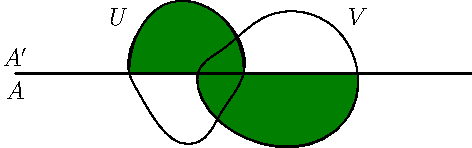
\includegraphics{NotesKonig_OpTern.pdf}
 % NotesKonig_OpTern.pdf: 182x198 px, 72dpi, 6.42x6.99 cm, bb=0 0 182 198
 \caption{Opération ternaire $U | A | V$}
 \label{fig:OpTern}
\end{figure}

\begin{propn}\label{Prop:OpTern}
 Soit $A, U, V, P, Q$ des parties d'un ensemble $X$.
 \begin{align}
  U \cap V &\subset U | A | V \subset U \cup V \\
  U | A | V &= V | A' | U \\
  (U | A | V)' &= U' | A | V' \\
  \left\lbrace
  \begin{aligned}
    P &= U | A | V \\
    Q &= V | A | U
  \end{aligned}
  \right.
  &\Leftrightarrow
  \left\lbrace
  \begin{aligned}
    U &= P | A | Q \\
    V &= Q | A | P
  \end{aligned}
  \right.
 \end{align}
\end{propn}
\begin{demo}
\begin{enumerate}
 \item $U \cap V = \left((U \cap V)\cap A'\right) \cup \left((U \cap V)\cap A\right)
 \subset \left( U \cap A'\right) \cup \left(V \cap A \right) = U | A | V$.
 \begin{displaymath}
  \left.
   \begin{aligned}
    U \cap A' &\subset U \\
    V \cap A &\subset V
   \end{aligned}
   \right\rbrace
   \Rightarrow
   U | A | V = \left( U \cap A'\right) \cup \left(V \cap A \right) \subset U \cup V.
 \end{displaymath}

 \item $U | A | V = \left( U \cap A'\right) \cup \left(V \cap A \right)
 = \left(V \cap A'' \right) \cup \left( U \cap A'\right) = V | A' | U$.

 \item La relation se lit sur la figure en considérant le complémentaire dans $A'$ et dans $A$. On l'obtient aussi en distribuant:
 \begin{multline*}
   (U | A | V)' =  \left(U' \cup A\right) \cap \left(V' \cup A' \right)
     = \left(\left(U' \cup A\right) \cap V'\right) \cup \left(\left(U' \cup A\right) \cap A'\right)\\
     = \left(U' \cap V' \right) \cup \left(A \cap V' \right)  \cup \left(U' \cap A' \right)
     = \left(U' \cap V' \right) \cup \left(U' | A | V'\right) = U' | A | V'
 \end{multline*}
à cause de la deuxième inclusion dans la première relation.

 \item Les parties $(P,Q)$ et $(U,V)$ jouent le même rôle. Il suffit de prouver une implication pour avoir l'équivalence.
 \begin{displaymath}
  \left\lbrace
  \begin{aligned}
   P &= U | A | V \\
   Q &= V | A | U
  \end{aligned}
  \right.
  \Rightarrow
  \left\lbrace
  \begin{aligned}
    P \cap A' &= U \cap A' \\
    Q \cap A &= U \cap A
  \end{aligned}
  \right.
  \Rightarrow P | A | Q = P.
 \end{displaymath}
De même pour $P \cap A$ et $Q \cap A'$.
\end{enumerate}

\end{demo}
\index{système de parties!treillis}
\begin{defin}
  Soit $\mathfrak{S}$ une partie de $\mathcal{P}(X)$
  \begin{itemize}
    \item $\mathfrak{S}$ est un treillis (lattice) si et seulement si $\mathfrak{S}$ est stable pour l'union et l'intersection.
    \item $\mathfrak{S}$ est un ovale (oval) si et seulement si $U$, $V$, $A$ dans $\mathfrak{S}$ entraine $U \mid A \mid V \in \mathfrak{S}$.\index{système de parties!ovale}
    \item $\mathfrak{S}$ est un anneau (ring) si et seulement si $\mathfrak{S}$ est stable pour l'union, l'intersection et la soustraction. La stabilité pour la soustraction signifie
    \begin{displaymath}
      \forall A, B \in \mathfrak{S}, B \subset A \Rightarrow A \setminus B = A \cap B' \in \mathfrak{S}.
    \end{displaymath}  \index{système de parties!anneau}
    \item $\mathfrak{S}$ est une algèbre (algebra) si et seulement si $\mathfrak{S}$ est stable pour l'union, l'intersection et la complémentation. \index{système de parties!algèbre}
  \end{itemize}
\end{defin}

\begin{propn}\label{prop:ImpTypesSyst}
  algèbre $\Rightarrow$ anneau $\Rightarrow$ ovale $\Rightarrow$ treillis
\end{propn}
\begin{demo}
Par exemple pour montrer qu'un anneau est un ovale, il suffit de remarquer qur
\begin{displaymath}
  U \mid A \mid V = (U \setminus (A \cap U)) \cup (A \cap V).
\end{displaymath}
Pour montrer qu'un ovale est un treillis:
\begin{align*}
  U \mid U \mid V = (U \cap U') \cup (U \cap V) = U \cap V \\
  U \mid V \mid V = (U \cap V') \cup (V \cap V) = U \cup V
\end{align*}
On vérifie facilement les autres implications.
\end{demo}

\begin{rems}
 \begin{enumerate}
  \item Un anneau contient toujours $\emptyset$ car $A \setminus A = \emptyset$.
  \item Un ovale qui contient $\emptyset$ est un anneau. En effet
    \begin{displaymath}
      U \mid A \mid \emptyset = (U \cap A')\cup (U \cap \emptyset) = U \cap A' = U \setminus A.
    \end{displaymath}
    Le fait qu'un anneau soit un ovale particulier (comme pour les figures géométriques) est la seule justification que j'ai trouvée pour le terme \emph{ovale}.
  \item Une algèbre contient toujours $\emptyset$ et $X$.
  \item Un anneau qui contient $X$ est une algèbre. En effet $A' = X \setminus A$.
  \item La stabilité pour l'union et la complémentation entraine la stabilité pour l'intersection car
  \begin{displaymath}
   A \cap B = \left(A' \cup B'\right)'.
  \end{displaymath}

 \end{enumerate}
\end{rems}
\begin{exples}
 Dans $\R$, l'ensemble des unions finies d'intervalles fermés est un treillis mais ce n'est pas un ovale. Par exemple, si $U = [0,2]$, $A=[1,4]$, $V = [3,5]$:
 \begin{displaymath}
  U|A|V = [0,1[ \, \cup \, [3,4]
 \end{displaymath}
n'est pas une union finie d'intervalles fermés.\newline
L'ensemble des unions finies d'intervalles fermés à gauche et ouverts à droite est un anneau. En effet, si $[x,y[ \subset [a,b[$,
\begin{displaymath}
 [a,b[ \,\setminus \, [x,y[ = [a,x[ \, \cup \, [b,y[.
\end{displaymath}
\end{exples}

\begin{propn}
  Pour tout système d'ensembles $\mathfrak{S}$ de $X$, l'ensemble des treillis (respectivement ovale, anneau, algèbre) contenant $\mathfrak{S}$ admet un plus petit élément pour l'inclusion noté $L(\mathfrak{S})$ (respectivement $O(\mathfrak{S}))$, $R(\mathfrak{S}))$, $A(\mathfrak{S}))$.
\end{propn}
\begin{demo}
Les structures sont définies par des stabilités. L'intersection de tous les treillis contenant $\mathfrak{S}$ vérifie les mêmes stabilités. C'est donc un treillis et il est contenu dans tous les treillis contenant $\mathfrak{S}$. Il en est de même pour les trois autres structures.
\end{demo}
D'après la proposition \ref{prop:ImpTypesSyst},
\begin{displaymath}
 A(\mathfrak{S}) \subset R(\mathfrak{S}) \subset O(\mathfrak{S}) \subset L(\mathfrak{S}).
\end{displaymath}

\subsection{Concepts vocabulaire notations}\label{SubSec:ConcVocNot}

\paragraph{Cardinalité}
Le premier concept est relatif à la cardinalité. L'auteur définit des notations très synthétiques avec un symbole $\bullet$ qui peut  désigner un des trois symboles $\star$, $\sigma$, $\tau$ que je ne reprendrai pas. J'utiliserai directement les 3 symboles pour préciser un caractère fini, dénombrable ou quelconque.\newline
Un système d'ensembles $\mathfrak{M}$ de $X$ est dit
\begin{itemize}
 \item de type $*$ si et seulement si il est fini;
 \item de type $\sigma$ si et seulement si il est fini ou dénombrable c'est à dire qu'existe une suite $(S_l)_{l\in \N}$ de parties de $X$ telles que $\mathfrak{M}= \left\lbrace S_l , l\in \N \right\rbrace$;
 \item de type $\tau$ dans tous les autres cas.
\end{itemize}
On peut remarquer que pour une famille de parties: \og~ type $*$~\fg{}\, entraine \og~ type $\sigma$ ~\fg{} \, entraine \og~ type $\tau$ ~\fg{}.

On peut aussi préfixer des propriétés. Par exemple, pour un système d'ensemble $\mathfrak{S}$ dans $X$;
\begin{align*}
\mathfrak{S} \text{ est $\cup_*$-stable } &\Leftrightarrow \left( \forall \mathfrak{M} \subset \mathfrak{S}, \mathfrak{M} \text{ fini } \Rightarrow \bigcup_{M \in \mathfrak{M}}M \in \mathfrak{S}.\right) \\
\mathfrak{S} \text{ est $\cup_\sigma$-stable } &\Leftrightarrow \left( \forall \mathfrak{M} \subset \mathfrak{S}, \mathfrak{M} \text{ dénombrable } \Rightarrow \bigcup_{M \in \mathfrak{M}}M \in \mathfrak{S}.\right) \\
\mathfrak{S} \text{ est $\cup_\tau$-stable } &\Leftrightarrow \left( \forall \mathfrak{M} \subset \mathfrak{S}, \bigcup_{M \in \mathfrak{M}}M \in \mathfrak{S}.\right)
\end{align*}
On peut remarquer que $\mathfrak{S}$ est $\cup_*$-stable si et seulement si $\mathfrak{S}$ est stable par $\cup$. Il est $\cup_\sigma$-stable si et seulement si, pour toute suite $(M_i)_{i\in \N}$ d'éléments de $\mathfrak{S}$, $\bigcup_{i\in \N}M_i \in \mathfrak{S}$.\newline
On définit de manière analogue les notions de $\cap_\star$-stable(équivalent à $\cap$-stable), $\cap_\sigma$-stable, $\cap_\tau$-stable.
\begin{rem}\label{rem:topologie}
 La topologie d'un ensemble $X$ est définie par l'ensemble de ses ouverts (noté $Op(X)$) c'est à dire un système d'ensembles contenant $\emptyset$ et $X$, $\cup_\tau$-stable, $\cap_\star$-stable.
\end{rem}
\begin{nota}
   Soit $\mathfrak{S}$ un système d'ensembles de $X$.\newline
   On note $\mathfrak{S}^{*}$ (respectivement $\mathfrak{S}^{\sigma}$, $\mathfrak{S}^{\tau}$) l'ensemble des $\bigcup_{S \in \mathfrak{M}}S$ où $\mathfrak{M}$ est une partie finie (respectivement dénombrable, quelconque ) de $\mathfrak{S}$.\newline
   On note $\mathfrak{S}_{*}$ (respectivement $\mathfrak{S}_{\sigma}$, $\mathfrak{S}_{\tau}$) l'ensemble des $\bigcap_{S \in \mathfrak{M}}S$ où $\mathfrak{M}$ est une partie finie (respectivement dénombrable, quelconque ) de $\mathfrak{S}$.
\end{nota}

\paragraph{Monotonie}

\begin{defin}\label{Def:monotonie}
   On note $(S_l)\uparrow$ pour indiquer qu'une suite de parties $S_l$ de $X$ est croissante c'est à dire $S_l \subset S_{l+1}$. De même $(S_l)\downarrow$ pour décroissante.
\index{système de parties! dirigé vers le haut}\index{système de parties! upward directed}\newline
   On note $\mathfrak{M}\uparrow$ pour indiquer qu'un système $\mathfrak{M}$ de parties de $X$ est dirigé vers le haut (upward directed) c'est à dire si et seulement si pour tous $U$ et $V$ dans $\mathfrak{M}$, il existe $W\in \mathfrak{M}$ tel que $U \cup V \subset W$.\newline
   On note $\mathfrak{M}\downarrow$ pour indiquer qu'un système $\mathfrak{M}$ de parties de $X$ est dirigé vers le bas (downward directed) c'est à dire si et seulement si pour tous $U$ et $V$ dans $\mathfrak{M}$, il existe $W\in \mathfrak{M}$ tel que $W \subset  U \cap V$.
\end{defin}

\begin{rems}
 \begin{enumerate}
  \item Un système de type $\tau$ stable pour $\cup$ (union) est dirigé vers le haut. Un système de type $\tau$ stable pour $\cap$ (union) est dirigé vers le bas.
  \item Un système $\mathfrak{M}$ de type $\tau$ est dirigé vers le haut si et seulement si toute partie finie de $\mathfrak{M}$ est majorée dans $\mathfrak{M}$. Un système $\mathfrak{M}$ de type $\tau$ est dirigé vers le bas si et seulement si toute partie finie de $\mathfrak{M}$ est minjorée dans $\mathfrak{M}$.
 \end{enumerate}
\end{rems}
\index{système de parties! dirigé vers le bas}\index{système de parties! downward directed}
\begin{defin}\label{Def:limMonotone}
  On note $\mathfrak{M}\uparrow S$ pour indiquer que $\mathfrak{M}$ est dirigé vers le haut avec $S = \bigcup_{M \in \mathfrak{M}}M$.\newline
  On note $\mathfrak{M}\downarrow S$ pour indiquer que $\mathfrak{M}$ est dirigé vers le bas avec $S = \bigcap_{M \in \mathfrak{M}}M$.
\end{defin}
\noindent Ces notations sont valables pour les $\tau$-systèmes comme pour les suites. Énonçons des propriétés des compacts avec ce vocabulaire.
\begin{exple} \label{systAproxCompact}
 Soit $K$ une partie compacte et $\mathfrak{M} = \left\lbrace K(\delta), \delta >0  \right\rbrace$. Alors $\mathfrak{M} \downarrow K$. Voir chapitre \ref{Chap:Outils} section \ref{Sec:EspMetric} prop  \ref{compactEtendu}.
\end{exple}
\begin{demo}
 Le seul point non évident est $\bigcap_{\delta > 0} K(\delta) \subset K$. Soit $x$ dans cette intersection. Pour tout naturel $n>0$,
 \begin{displaymath}
  x \in K(\frac{1}{n}) \Rightarrow \exists x_n \in K \text{ tq } d(x,x_n) < \frac{1}{n}.
 \end{displaymath}
Comme $K$ est compact, on peut extraire de la suite $(x_n)$ d'éléments de $K$ une suite $(x_{\varphi(n)})$ qui converge vers un $a\in K$. On en déduit $d(x,a)=0$ donc $x=a \in K$.
\end{demo}
\begin{propn}\label{Prop:SegEmboit}
 Soit $\mathfrak{M}\downarrow \emptyset$ un système de parties compactes dirigé vers le bas. Il existe $N \in \mathfrak{M}$ tel que $N = \emptyset$.
\end{propn}
\begin{demo}
Fixons un compact $M\in \mathfrak{M}$ et notons $\mathfrak{N}$ l'ensemble des $N\in \mathfrak{M}$ tels que $N \subset M$. C'est encore un système de parties dirigé vers le bas. Alors
\begin{displaymath}
 M \setminus \left( \bigcup_{N \in \mathfrak{N}} M\setminus N\right)
 =  M \cap \left( \bigcap_{N \in \mathfrak{N}} (M' \cup N)\right)
 =  M \cap \left( M' \cup \bigcap_{N \in \mathfrak{N}}  N\right)
 =  M \cap  \bigcap_{N \in \mathfrak{N}}N
 = \bigcap_{N \in \mathfrak{N}}N
\end{displaymath}
car $M \in \mathfrak{N}$. On en déduit
\begin{displaymath}
 \bigcap_{N \in \mathfrak{N}}N = \emptyset \Rightarrow M = \bigcup_{N \in \mathfrak{N}} M\setminus N.
\end{displaymath}
Les $M\setminus N$ forment un recouvrement du compact $M$ par des parties ouvertes de $M$ car les $N$ sont des fermés. On peut en extraire un recouvrement fini. Il existe $N_1, \cdots, N_p$ tels que
\begin{displaymath}
 M = (M\setminus N_1) \cup \cdots \cup (M\setminus N_p).
\end{displaymath}
Comme $\mathfrak{M}$ est dirigé vers le bas, il existe $N \in \mathfrak{M}$ tel que $N \subset N_1 \cap \cdots N_p$ donc $M \setminus N_i \subset M \setminus N$ pour tous les $i$. On en déduit $M \subset M \setminus N$ donc $N = \emptyset$.
\end{demo}
Cette proposition est une généralisation abstraite du théorème des segments emboîtés: l'intersection d'une suite de segments emboités est un segment non vide.

\paragraph{Stabilités monotones}
\begin{defi}
Pour un système d'ensembles $\mathfrak{S}$ dans $X$, on définit quatre propriétés de stabilités monotones notées $\uparrow \sigma$, $\downarrow \sigma$, $\uparrow \tau$, $\downarrow \tau$.
\begin{align*}
 \mathfrak{S} \text{ vérifie } \uparrow \sigma &\Leftrightarrow
   \left( \text{Pour toute suite } (S_l) \text{ d'éléments de } \mathfrak{S}, (S_l)\uparrow S  \text{ entraine } S \in \mathfrak{S} \right), \\
 \mathfrak{S} \text{ vérifie } \downarrow \sigma &\Leftrightarrow
   \left( \text{Pour toute suite } (S_l) \text{ d'éléments de } \mathfrak{S}, (S_l)\downarrow S  \text{ entraine } S \in \mathfrak{S} \right), \\
 \mathfrak{S} \text{ vérifie } \uparrow \tau &\Leftrightarrow
   \left( \text{Pour tout } \mathfrak{M} \subset \mathfrak{S}, \mathfrak{M}\uparrow S  \text{ entraine } S \in \mathfrak{S} \right), \\
 \mathfrak{S} \text{ vérifie } \downarrow \tau &\Leftrightarrow
   \left( \text{Pour tout } \mathfrak{M} \subset \mathfrak{S}, \mathfrak{M}\downarrow S  \text{ entraine } S \in \mathfrak{S} \right), \\
\end{align*}
\end{defi}
\index{système de parties! $\sigma$ treillis}\index{système de parties! $\sigma$ ovale} \index{système de parties! $\sigma$ anneau} \index{système de parties! $\sigma$ algèbre}
\begin{defin}
\begin{itemize}
 \item Un $\sigma$-treillis est un treillis qui vérifie $\uparrow \sigma$ et $\downarrow \sigma$.
 \item Un $\sigma$-ovale est un ovale qui vérifie $\uparrow \sigma$ et $\downarrow \sigma$.
 \item Un $\sigma$-anneau est un anneau qui vérifie $\uparrow \sigma$ et $\downarrow \sigma$.
 \item Une $\sigma$-algèbre est une algèbre qui vérifie $\uparrow \sigma$ et $\downarrow \sigma$.
\end{itemize}
\end{defin}
\index{tribu}
\begin{rems}
\begin{enumerate}
 \item Une $\sigma$-algèbre est aussi appelée \emph{tribu} en français.
 \item Soit $\mathfrak{S}$ un système de parties de $X$. Pour toute suite $(S_l)$ croissante d'éléments de $\mathfrak{S}$,
   \begin{displaymath}
     (S_l)\uparrow S \Leftrightarrow  S = \bigcup_l S_l.
   \end{displaymath}
  On en déduit que $\mathfrak{S}$ vérifie $\uparrow \sigma$ si et seulement si $\mathfrak{S}$ est $\bigcup - \sigma$-stable si et seulement si $\mathfrak{S}^\sigma = \mathfrak{S}$.
 \item L'intersection d'une famille de système $\uparrow \sigma$ stables (resp $\downarrow \sigma$ stables) est $\uparrow \sigma$ stable (resp $\downarrow \sigma$ stable).
 \item Pour tout système d'ensembles $\mathfrak{S}$, il existe donc un plus petit treillis (resp ovale, anneau, algèbre) contenant $\mathfrak{S}$. Il est noté $L_\sigma(\mathfrak{S})$ (resp $O_\sigma(\mathfrak{S})$, $R_\sigma(\mathfrak{S})$, $A_\sigma(\mathfrak{S})$) et appelé treillis (resp ovale, anneau, algèbre) engendré par $\mathfrak{S}$.
\end{enumerate}
\end{rems}
\index{$\sigma$-algèbre de Borel}\index{tribu borelienne}
\begin{exple}
Lorsque $\mathfrak{S}$ est l'ensemble des ouverts d'un espace topologique $X$, la $\sigma$-algèbre $A_\sigma(\mathfrak{S})$ engendrée par $\mathfrak{S}$ est appelée $\sigma$-algèbre de Borel ou tribu borelienne.
\end{exple}

\begin{defin}[parties cloturables]\label{Def:cloturable} \index{parties cloturables} \index{notations!$\sqsubset \mathfrak{T}$, $\sqsupset \mathfrak{T}$, $\mathfrak{S} \sqsubset \mathfrak{T}$}
 Soit $\mathfrak{T}$ un système de parties de $X$. Une partie $A$ de $X$ est dite $\mathfrak{T}$-cloturable vers le haut (resp vers le bas) si et seulement si il existe $T\in \mathfrak{T}$ tel que $A \subset T$ (resp $T \subset A$).\newline
 L'ensemble des parties $\mathfrak{T}$-cloturables vers le haut (resp vers le bas) est noté $\sqsubset \mathfrak{T}$ (resp $\sqsupset \mathfrak{T}$).\newline
 Soit $\mathfrak{S}$ et $\mathfrak{T}$ deux systèmes de parties de $X$. On note $\mathfrak{S} \sqsubset \mathfrak{T} = (\sqsupset \mathfrak{S}) \cap (\sqsubset \mathfrak{T})$ le systèmes des parties de $X$ caractérisées par: pour tout $A\subset X$,
 \begin{displaymath}
  A \in \mathfrak{S} \sqsubset \mathfrak{T} \Leftrightarrow
  \exists S \in \mathfrak{S}, \exists T \in \mathfrak{T} \text{ tels que } S \subset A \subset T.
 \end{displaymath}
\end{defin}

\section{Fonctions d'ensembles}\label{Sec:FoncEns}
\subsection{Croissance et modularité} \label{SubSec:CroissModul}
Page 10. L'auteur considère des fonctions définies dans un treillis $\mathfrak{S}$ d'un ensemble $X$ et à valeurs dans $\overline{\R}= \R \cup\{- \infty, + \infty\} $. On peut étendre l'addition à $\overline{\R}$ de deux manières: en convenant que $(+ \infty) + (-\infty) = + \infty$ ou que $(+ \infty) + (-\infty) = - \infty$ en plus des règles usuelles. Dans les deux cas, l'addition étendue est associative et commutative.

\begin{defi}
  Une fonction $\varphi$ définie dans un treillis $\mathfrak{S}$ à valeurs dans $\overline{\R}$ est dite croissante (isotone) si et seulement si
  \begin{displaymath}
    \forall (A,B) \in \mathfrak{S},\; A \subset B \Rightarrow \varphi(A) \leq \varphi(B).
  \end{displaymath}
\end{defi}
\noindent En général, les fonctions d'ensembles considérées sont croissantes.

\begin{defi}
  Une fonction $\varphi$ définie dans un treillis $\mathfrak{S}$ à valeurs dans $\overline{\R}$ est dite modulaire pour une extension de l'addition si et seulement si
\begin{displaymath}
  \forall (A,B) \in \mathfrak{S}^2, \varphi(A \cup B) + \varphi(A \cap B) = \varphi(A) + \varphi(B)
\end{displaymath}
pour cette extension. De même
\begin{align*}
  \varphi \text{ est sous-modulaire } &\Leftrightarrow \forall (A,B) \in \mathfrak{S}^2, \varphi(A \cup B) + \varphi(A \cap B) \leq \varphi(A) + \varphi(B) \\
  \varphi \text{ est sur-modulaire } &\Leftrightarrow \forall (A,B) \in \mathfrak{S}^2, \varphi(A \cup B) + \varphi(A \cap B) \geq \varphi(A) + \varphi(B)
\end{align*}
\end{defi}

  \noindent On convient de noter $\overset{\circ}{+}$ l'extension de l'addition vérifiant $(-\infty) \overset{\circ}{+} (+\infty) = +\infty$ et $\underset{\circ}{+}$ l'extension de l'addition vérifiant $(-\infty) \underset{\circ}{+} (+\infty) = -\infty$. \newline
  Exercice 2.8 (p 13). La modularité dépend vraiment de l'extension choisie.
  \begin{enumerate}
    \item Sur $\mathfrak{S} = \mathcal{P}(X)$ où $X$ est un ensemble à deux éléments, définir une fonction $\varphi$ croissante et modulaire pour $\underset{\circ}{+}$ mais pas sous-modulaire pour $\overset{\circ}{+}$.
    \item Soit $\varphi$ croissante de $\mathfrak{S}$ dans $\overline{\R}$, montrer que
\begin{displaymath}
  \varphi \text{ sous-modulaire pour } \overset{\circ}{+} \Rightarrow \varphi \text{ sous-modulaire pour } \underset{\circ}{+}.
\end{displaymath}
  \end{enumerate}
  \begin{demo}
  \begin{enumerate}
    \item Soit $X=\{a,b\}$ un ensemble à 2 éléments. On définit $\varphi$ dans $\mathcal{P}(X)$ par $\varphi(X) = +\infty$ et $\varphi(A) = - \infty$ pour toutes les autres parties $A$ de $X$. La fonction est bien $\underset{\circ}{+}$ modulaire car la somme des images par $\varphi$ de deux parties distinctes sera toujours $-\infty$ sauf si $A=B=X$. En revanche, elle n'est pas $\overset{\circ}{+}$ sous-modulaire car
    \begin{displaymath}
      \varphi(\{a\}\cup \{b\}) \overset{\circ}{+} \varphi(\{a\}\cap \{b\}) = (+\infty) \overset{\circ}{+} (-\infty) = + \infty
    \end{displaymath}
    n'est pas inférieur ou égal à
    \begin{displaymath}
      \varphi(\{a\}) \overset{\circ}{+} \varphi(\{b\}) = (-\infty) \overset{\circ}{+} (-\infty) = - \infty.
    \end{displaymath}

    \item On forme un tableau en plaçant dans les deux premières colonnes toutes les situations possibles pour les valeurs de $\varphi(A)$ et $\varphi(B)$ en tenant compte des symétries. On peut remplir beaucoup de cases dans  les autres colonnes en utilisant les conséquences de la croissance et de la sous-modularité pour $\overset{\circ}{+}$ de $\varphi$. On laisse vide les cases pour lesquelles on ne peut rien déduire.
\begin{center}
\begin{tabular}{lllllll}
$\varphi(A)$ & $\varphi(B)$ & $\varphi(A\cup B)$ & $\varphi(A\cap B)$ & $\varphi(A) \overset{\circ}{+} \varphi(B)$ & $\varphi(A\cup B) \underset{\circ}{+} \varphi(A\cap B)$ & $\varphi(A) \underset{\circ}{+} \varphi(B)$\\ \hline
$-\infty$    & $-\infty$    &                    & $-\infty$          & $-\infty$                              & $-\infty$   & $-\infty$ \\  \hline
$-\infty$    & $\in \R$     & $> -\infty$        & $-\infty$          & $-\infty$                              & $-\infty$   & $-\infty$ \\ \hline
$-\infty$    & $+\infty$    & $+\infty$          & $-\infty$          & $+\infty$                              & $-\infty$   & $-\infty$\\ \hline
$\in \R$     & $\in \R$     & $\in \R$           & $< +\infty$        & $\in \R$                               & $< +\infty$ & $\in \R$\\ \hline
$\in \R$     & $+\infty$    & $+\infty$          & $< +\infty$        & $+\infty$                              & $< +\infty$ & $+\infty$ \\ \hline
$+\infty$    & $+\infty$    & $+\infty$          &                    & $+\infty$                              &             & $+\infty$\\ \hline
\end{tabular}
\end{center}
  \end{enumerate}
  \end{demo}
La comparaison des deux dernières colonnes montre que l'inégalité caractérisant la sous-modularité $\underset{\circ}{+}$ est toujours vérifiée.\newline
Dans le cas $\varphi(A)$ et $\varphi(B)$ réels, si $\varphi(A\cap B)$ est réel, les 4 termes sont réels, l'addition dans l'inégalité est l'addition habituelle. Si $\varphi(A\cap B) = - \infty$,  $\varphi(A\cup B) \underset{\circ}{+} \varphi(A\cap B) = -\infty$ donc l'inégalité est vérifiée.\newline
Dans le cas où $\varphi(A)$ et $\varphi(B)$ valent $+\infty$, peu importe la valeur de $\varphi(A\cup B) \underset{\circ}{+} \varphi(A\cap B)$, elle sera toujours $\leq +\infty$.
Venons en aux formules qui ressemblent au crible de Poincaré (exercie 2.5 du livre). On reprend les notations de la partie \ref{Sec:criblePoinc} du chapitre \ref{Chap:Outils}.
\begin{propn}\label{modulaire_ordre_n}
  Soit $\varphi$ une fonction modulaire sur un treillis $\mathfrak{S}$ et $A_1, \cdots , A_p$ dans $\mathfrak{S}$:
  \begin{displaymath}
    \varphi(\bigcup_{i=1}^p A_i) = - \sum_{I \subset \llbracket 1,p \rrbracket, I\neq \emptyset} (-1)^{\sharp I}\varphi(A_I).
  \end{displaymath}
\end{propn}
\begin{demo}
  Pour $p=2$, les parties $I$ intervenant sont $\{1\}$, $\{2\}$ et $\{1,2\}$. la formule à montrer s'écrit
  \begin{displaymath}
    \varphi(A_1 \cup A_2) = - \left( -\varphi(A_1) - \varphi(A_2) + \varphi(A_1\cap A_2)\right)
  \end{displaymath}
qui est la définition de la modularité.\newline
Montrons que la formule à l'ordre $p$ entraine celle à l'ordre $p+1$. Partons de la somme à l'ordre $p+1$ et trions les $I$ : ceux qui ne contiennent pas $p+1$, ceux qui le contiennent entre autres et le singleton $\{p+1\}$:
\begin{align*}
  - \sum_{I \subset \llbracket 1,p+1 \rrbracket, I\neq \emptyset} (-1)^{\sharp I}\varphi(A_I)
  = - \sum_{I \subset \llbracket 1,p \rrbracket, I\neq \emptyset} (-1)^{\sharp I}\varphi(A_I)
  + \sum_{J \subset \llbracket 1,p \rrbracket, J\neq \emptyset} (-1)^{\sharp J}\varphi(A_I \cap A_{p+1})
  + \varphi(A_{p+1}) \\
  = \varphi(\bigcup_{i=1}^p A_i) - \varphi(\bigcup_{i=1}^p A'_i) + \varphi(A_{p+1})
  = \varphi(\bigcup_{i=1}^p A_i) + \varphi(A_{p+1}) -\varphi(\left(\bigcup_{i=1}^p A_i\right) \cap A_{p+1})
  = \varphi(\bigcup_{i=1}^{p+1} A_i)
\end{align*}
en utilisant $A'_i = A_i  \cap A_{p+1}$ pour $i \in \llbracket 1, p \rrbracket$ puis l'hypothèse de récurrence (deux fois) et enfin la définition de la modularité.
\end{demo}
\begin{rem}
  Cette formule fournit une nouvelle démonstration de la formule du crible. En effet dans un ensemble $X$, la fonction de Dirac $\delta_x$ définie par
  \begin{displaymath}
     \forall A \subset X, \;\delta_x(A) =
    \left\lbrace
    \begin{aligned}
      1 &\text{ si } x \in A \\
      0 &\text{ si } x \notin A
    \end{aligned}
    \right.
  \end{displaymath}
  est modulaire. Elle est liée aux fonctions caractéristiques par: $\delta_x(A) = \chi_A(x)$. On en déduit
  \begin{displaymath}
    \left( \forall x \in X, \; \delta_x(\bigcup_{i=1}^p A_i) = - \sum_{I \subset \llbracket 1,p \rrbracket, I\neq \emptyset} (-1)^{\sharp I}\delta_x(A_I) \right)
    \Rightarrow  \chi_{\bigcup_{i=1}^p A_i} = - \sum_{I \subset \llbracket 1,p \rrbracket, I\neq \emptyset} (-1)^{\sharp I}\chi_{A_I}.
  \end{displaymath}
\end{rem}
\begin{rem}
 À cause de l'alternance des signes, cette formule ne subsiste pas dans le cas d'une fonction seulement sous-modulaire. Signalons dans le chapitre \ref{Chap:ExtenRegul} section \ref{Sec:Enveloppes} sous-section \ref{SubSec:EnvlpExterieures}, l'inégalité du lemme \ref{Lemm:InegSousModul} qui est du même genre et joue un rôle important dans la démonstration du théorème \ref{Theor:ContEnvlp} .
\end{rem}

\subsection{Extension d'une fonction d'ensembles à un treillis}
Dans cette section l'ouvrage considère une fonction d'ensembles $\varphi$ définie sur un ensemble $\mathfrak{U}$ de parties de $X$ seulement stable pour l'intersection et cherche à la prolonger en une fonction modulaire $\phi$ sur $\mathfrak{S} = L(\mathfrak{U})$ qui est le plus petit treillis contenant $\mathfrak{U}$.

Cette situation est celle du premier exemple où $\mathfrak{U}$ est l'ensemble formé du vide et des classes de congruences autres que $\{0\}$. Cet ensemble est stable par intersection et l'ensemble $\mathfrak{S}$ des unions de classes de congruences est le plus petit treillis contenant $\mathfrak{U}$.
Au départ, la fonction $\varphi$ est définie uniquement sur $\mathfrak{U}$ par  $\varphi(a + \Z m) = \frac{1}{m}$.
Peut-on l'étendre à une fonction modulaire sur $\mathfrak{S}$ ? On l'a fait à l'aide du cardinal des images par les projections canoniques donc je n'ai pas besoin des résultats de cette section pour cet exemple.

Je reproduis quand même ici ces résultats et leurs preuves(pages 27 à 31).

L'ouvrage définit pour tous les $n$ des fonctions notées encore $\varphi$ de $\mathfrak{U}^n$ dans $\R$ inspirées des formules d'inclusion-exclusion
\begin{displaymath}
  \forall n \in \N^*, \forall (A_1,\cdots, A_n) \in \mathfrak{U}^n, \;
  \varphi(A_1, \cdots, A_n) = - \sum_{\emptyset \neq I \subset \llbracket 1 , n\rrbracket}(-1)^{\sharp(I)}\varphi(A_I)
\end{displaymath}
où $A_I$ est défini comme dans la section précédente par $A_I = \bigcap_{i\in I} A_I$.
\begin{rem}
  Ces fonctions sont clairement symétriques, permuter les $A_i$ ne change pas la valeur.
\end{rem}

\begin{prop}
  \begin{enumerate}
    \item Formule de récurrence. Soit $A_0, \cdots, A_r$ des éléments de $\mathfrak{U}$ :
    \begin{displaymath}
      \varphi(A_0,\cdots, A_r) = \varphi(A_0) + \varphi(A_1,\cdots, A_r) - \varphi(A_0\cap A_1, \cdots, A_0\cap A_r).
    \end{displaymath}
    \item Soit $A_0, \cdots, A_r$ des éléments de $\mathfrak{U}$ tels que $A_i \subset A_0$ pour tous les $i$ :
    \begin{displaymath}
      \varphi(A_0,\cdots, A_r) = \varphi(A_0).
    \end{displaymath}
    \item Soit $A_0, \cdots, A_r$ des éléments de $\mathfrak{U}$ tels qu'il existe $l \in \llbracket 1, r \rrbracket$ vérifiant $A_0 \subset A_l$
    \begin{displaymath}
      \varphi(A_0,A_1, \cdots,A_r) = \varphi(A_1, \cdots,A_r).
    \end{displaymath}
    \item Soit $A_1, \cdots, A_r, B_1, \cdots, B_s$ des éléments de $\mathfrak{U}$ :
    \begin{align*}
      \varphi(A_1, \cdots, A_r, B_1, \cdots, B_s) + \varphi(A_1\cap B_1, \cdots, A_r\cap B_s) \\
      = \varphi(A_1,\cdots,A_r) + \varphi(B_1, \cdots, B_s)
    \end{align*}
où l'argument du second terme de la somme à gauche de l'égalité est la suite des $rs$ intersections $A_i \cap B_j$ pour $i \in \llbracket 1,r \rrbracket$ et $i \in \llbracket 1,s \rrbracket$.
  \end{enumerate}
\end{prop}

\begin{demo}
  \begin{enumerate}
    \item On classe les parties $I$ en trois catégories: $\{ 0 \}$, les parties non vides ne contenant pas $0$, celles contenant $0$ et d'autres éléments. Ces dernières sont de la forme $I = \{ 0 \}\cup J$ avec $\emptyset \neq J \subset \llbracket 1, r \rrbracket$ avec $\sharp(J) = \sharp(I) -1$. La décomposition de la somme conduit à la formule.
    \item On applique la première formule avec $A_0 \cap A_i = A_i$.
    \item Par symétrie, on peut supposer $A_0 \subset A_1$. Pour $r = 1$, $A_0 \cap A_1 = A_0)$
    \begin{displaymath}
      \varphi(A_0, A_1) = \varphi(A_0) + \varphi(A_1) - \varphi(A_0) = \varphi(A_1).
    \end{displaymath}
    Pour $r\geq 2$.
    \begin{displaymath}
      \varphi(A_0,A_1, \cdots,A_r) = \varphi(A_0) + \varphi(A_1, \cdots,A_r) - \varphi(A_0,A_0 \cap A_2, \cdots , A_0\cap A_r) = \varphi(A_1, \cdots,A_r)
    \end{displaymath}
    d'après 2.
    \item On procède par récurrence sur $r$. Pour $r=1$ la formule est la même que celle du 1.\newline
    Pour passer de $r$ à $r+1$, on considère $(A_0, \cdots,A_r)$ et la famille des $(r+1)\times s$ intersections transformée par la formule 1 en adjoignant $A_0$.
    \begin{multline*}
      \varphi(A_0\cap B_1, \cdots, A_r \cap B_s) \\
      = \varphi(A_0, A_0\cap B_1, \cdots, A_r \cap B_s) -\varphi(A_0) + \varphi(A_0\cap A_0\cap B_1, \cdots, A_0\cap A_r \cap B_s)\\
      = \varphi \left(
      \begin{aligned}
      &A_0, \\
      &A_0 \cap B_1, \cdots, A_0\cap B_s, \\
      &A_1 \cap B_1, \cdots, A_1\cap B_s, \\
      & \vdots  \\
      &A_r \cap B_1, \cdots, A_r\cap B_s
      \end{aligned}
      \right)
      -\varphi(A_0)
      + \varphi \left(
      \begin{aligned}
        & A_0\cap B_1, &\cdots &, A_0 \cap B_s, \\
        &A_0\cap A_1\cap B_1, &\cdots &, A_0\cap A_1 \cap B_s, \\
        & \vdots \\
        &A_0\cap A_r\cap B_1, &\cdots &, A_0\cap A_r \cap B_s
      \end{aligned}
      \right)
    \end{multline*}
    On utilise la propriété 3 qui permet de supprimer les termes qui ne contribuent pas quand ils sont inclus dans une autre partie de la famille.\newline
    Dans le tableau de gauche, toutes les parties de la deuxième ligne sont incluses dans $A_0$. On peut donc supprimer cette deuxième ligne.\newline
    Dans le tableau de droite, les parties figurant dans une colonne sont incluses dans la partie figurant en haut de la colonne. On peut donc supprimer toutes les lignes sauf la première. On obtient
    \begin{multline*}
      \varphi(A_0\cap B_1, \cdots, A_r \cap B_s)
      = \varphi(A_0, A_1 \cap B_1, \cdots A_r \cap B_s) - \varphi(A_0) + \varphi(A_0\cap B_1, \cdots A_0 \cap B_s) \\
      = \varphi( A_1 \cap B_1, \cdots A_r \cap B_s) - \varphi(A_0 \cap A_1 \cap B_1, \cdots, A_0 \cap A_r \cap B_s) + \varphi(A_0\cap B_1, \cdots A_0 \cap B_s)
    \end{multline*}
    En utilisant encore la formule 1 avec les deux premiers termes. On est alors en mesure d'utiliser deux fois l'hypothèse de récurrence. D'abord avec le premier terme
    \begin{displaymath}
      \varphi( A_1 \cap B_1, \cdots, A_r \cap B_s)
      = \varphi( A_1, \cdots, A_r) + \varphi( B_1, \cdots , B_s) - \varphi( A_1, \cdots, A_r, B_1, \cdots , B_s)
    \end{displaymath}
    puis avec les deux derniers que l'on réécrit d'abord avec $A'_i = A_0 \cap A_i$ pour $i \in \llbracket 1, r \rrbracket$ et $B'_j = A_0 \cap B_j$ pour $j \in \llbracket 1, s \rrbracket$.
    \begin{align*}
      - \varphi( A'_1 \cap B'_1, \cdots,  A'_r \cap B'_s) + \varphi( B'_1, \cdots, B'_s)
      = - \varphi( A'_1, \cdots, A'_r) + \varphi( A'_1, \cdots, A'_r, B'_1, \cdots, B'_s) \\
      = - \varphi( A_0\cap A_1, \cdots, A_0 \cap A_s) + \varphi( A_0 \cap A_1, \cdots, A_0 \cap A_r, A_0 \cap B_1, \cdots, A_0 \cap B_s)\\
      = \varphi(A_0, \cdots, A_r) - \varphi(A_0) - \varphi(A_1, \cdots, A_r)
       - \varphi(A_0, \cdots, A_r,B_1, \cdots, B_s) + \varphi(A_0) \\
       + \varphi(A_1, \cdots, A_r,B_1, \cdots, B_s)
    \end{align*}
    en utilisant encore deux fois la propriété 1 avec $A_0$ en premier. En rassemblant, après simplifications, il reste seulement
    \begin{displaymath}
      \varphi(A_0\cap B_1, \cdots, A_r \cap B_s)
      = \varphi( B_1, \cdots , B_s) + \varphi(A_0, \cdots, A_r) - \varphi(A_0, \cdots, A_r,B_1, \cdots, B_s)
    \end{displaymath}
    qui est bien la formule de récurrence à l'ordre $r+1$.
  \end{enumerate}
\end{demo}
Le principal résultat de cette section est le théorème suivant.
\begin{thm}
  La fonction $\varphi$ de $\mathfrak{U}$ dans $\R$ admet une extension modulaire $\phi$ de $\mathfrak{S}$ dans $\R$ si et seulement si pour chaque $A_1, \cdots,A_p,A$ dans $\mathfrak{U}$ tels que $A_1 \cup \cdots \cup A_p = A$,
  \begin{displaymath}
    \varphi(A_1, \cdots,A_p) = \varphi(A).
  \end{displaymath}
  Nommons $(mod)$ cette condition. Dans ce cas la fonction $\phi$ est définie par
  \begin{displaymath}
    \forall A \in \mathfrak{S}, \phi(A) = \varphi(A_1,\cdots, A_p) \text{ où } A = A_1 \cup \cdots \cup A_p \text{ avec }(A_1,\cdots,A_p) \in \mathfrak{U}^p.
  \end{displaymath}
  De plus $\phi$ est croissante (isotone) si et seulement si, pour tous $A_1, \cdots, A_p, A$ dans $\mathfrak{U}$,
  \begin{displaymath}
    A_1 \cup \cdots \cup A_p \subset A \Rightarrow \varphi(A_1, \cdots, A_p) \leq \varphi(A).
  \end{displaymath}
  Nommons $(isot)$ cette condition.
\end{thm}
\begin{demo}
  À cause de la proposition \ref{modulaire_ordre_n} qui exprime $\varphi(A_1, \cdots, A_p) = \varphi(A_1,\cdots,A_p)$ les deux conditions $(mod)$ et $(isot)$ sont nécessaires.\newline
  Montrons que la condition
  \begin{displaymath}
    \text{(mod)} \; \forall A_1, \cdots,A_p,A \in \mathfrak{U}, A_1 \cup \cdots \cup A_p = A \Rightarrow
    \varphi(A_1, \cdots,A_p) = \varphi(A)
  \end{displaymath}
  permet d'étendre $\varphi$ en $\phi$. Il s'agit de montrer que
  \begin{displaymath}
    A = A_1 \cup \cdots \cup A_p = B_1 \cup \cdots \cup B_p \Rightarrow \varphi(A_1, \cdots, A_p) = \varphi(B_1, \cdots, B_p).
  \end{displaymath}
  Commençons par une conséquence de (mod), pour tous $A_0, A_1, \cdots, A_p \in \mathfrak{U}$:
  \begin{displaymath}
    A_0 \subset A_1 \cup \cdots \cup A_p \Rightarrow \varphi(A_0,A_1, \cdots, A_p) = \varphi(A_1, \cdots, A_p).
  \end{displaymath}
  En effet
  \begin{align*}
    A_0 \subset A_1 \cup \cdots \cup A_p \Rightarrow A_0 = (A_0\cap A_1) \cup \cdots \cup (A_0 \cap A_p) \\
      \Rightarrow \varphi(A_0) = \varphi((A_0\cap A_1) \cup \cdots \cup (A_0 \cap A_p)) \text{ d'après (mod)} \\
      \Rightarrow \varphi(A_0,A_1, \cdots, A_p) - \varphi(A_1, \cdots, A_p) = \varphi(A_0) - \varphi((A_0\cap A_1) \cup \cdots \cup (A_0 \cap A_p) = 0
  \end{align*}
  d'après la propriété 1. Si $A_1 \cup \cdots \cup A_p = B_1 \cup \cdots \cup B_p$ alors chaque $B_i$ est inclus dans l'union des $A_i$ donc, en les ajoutant un par un:
  \begin{displaymath}
    \varphi(A_1, \cdots, A_p) = \varphi(A_1, \cdots, A_p, B_0, \cdots, B_p) = \varphi(B_1, \cdots, B_p).
  \end{displaymath}
  Pour montrer la croissance de $\phi$, il suffit de montrer que pour $A_0, A_1, \cdots, A_p$ dans $\mathfrak{U}$,
  \begin{displaymath}
    \phi(A_1\cup \cdots \cup A_p) \leq \phi(A_0 \cup A_1 \cup \cdots \cup A_p).
  \end{displaymath}
  Or
  \begin{align*}
    \phi(A_0 \cup A_1 \cup \cdots \cup A_p) - \phi(A_1\cup \cdots \cup A_p)
    = \varphi(A_0, \cdots, A_p) - \varphi(A_1, \cdots, A_p)\\
    = \varphi(A_0) - \varphi(A_0\cap A_1, \cdots, A_0\cap A_p) \geq 0
  \end{align*}
d'après l'hypothèse car $(A_0 \cap A_1) \cup \cdots \cup (A_0\cap A_p) \subset A_0$.
\end{demo}


\subsection{Régularité} \label{SubSec:Regularite}
\noindent Soit $\varphi$ une fonction isotone d'ensembles de $\mathfrak{S}$ dans $\overline{\R}$.
Pour tout $S \in \mathfrak{S}$, on a évidemment
\begin{displaymath}
 \varphi(S) = \inf\left\lbrace \lambda(M), M \in \mathfrak{S}, S \subset M\right\rbrace \text{ et }
 \varphi(S) = \sup\left\lbrace \lambda(M), M \in \mathfrak{S}, M \subset S\right\rbrace.
\end{displaymath}
C'est même le plus petit élément de $\left\lbrace \lambda(M), M \in \mathfrak{S}, S \subset M\right\rbrace$ ou le plus grand de $\left\lbrace \lambda(M), M \in \mathfrak{S}, M \subset S \right\rbrace$. Pour certains $S$, on peut réduire l'ensemble dans lequel on considère les $M$ contenant (ou contenus dans) $S$.\newline
On se donne 3 systèmes d'ensembles $\mathfrak{M}$, $\mathfrak{S}$, $\mathfrak{T}$ avec $\mathfrak{M} \subset \mathfrak{S}$ et $\mathfrak{T} \subset \mathfrak{S}$. La fonction d'ensembles $\varphi$ est dite extérieurement $\mathfrak{M}$-régulière en $\mathfrak{T}$ si et seulement si
\begin{displaymath}
 \forall S \in \mathfrak{T}, \varphi(S) = \inf\left\lbrace \varphi(M), M \in \mathfrak{M} \text{ avec } S \subset M\right\rbrace.
\end{displaymath}
On dira que $\varphi$ est intérieurement $\mathfrak{M}$-régulière en $\mathfrak{T}$ si et seulement si
\begin{displaymath}
 \forall S \in \mathfrak{T}, \varphi(S) = \sup\left\lbrace \varphi(M), M \in \mathfrak{M} \text{ avec } M \subset S\right\rbrace.
\end{displaymath}
Conventions usuelles: $\inf \emptyset = + \infty$, $\sup \emptyset = - \infty$.\newline
Le cas le plus fréquent est $\mathfrak{T} = \mathfrak{S}$. On dit alors que $\varphi$ est (intérieurement, extérieurement) $\mathfrak{M}$-régulière.

\noindent La fonction d'ensembles $\varphi$ est dite
\begin{itemize}
 \item majorée (bounded above) si et seulement si il existe $c\in \R$ tel que $\varphi \leq c$,
 \item finie supérieurement (finite above) si et seulement si $\varphi < +\infty$,
 \item semi finie supérieurement (semifinite above) si et seulement si elle est intérieurement $\left\lbrace \varphi < + \infty\right\rbrace$-régulière.
\end{itemize}
\begin{rems}
 \begin{enumerate}
  \item $\varphi$ semi finie supérieurement si et seulement si pour tout $S \in \mathfrak{S}$,
  \begin{displaymath}
   \varphi(S) = \sup\left\lbrace \varphi(M)\text{ tq } M \subset S, \varphi(M) \in \R  \right\rbrace.
  \end{displaymath}
  \item majorée $\Rightarrow$ finie supérieurement $\Rightarrow$ semi finie supérieurement.
 \end{enumerate}
\end{rems}


\subsection{Continuités} \label{SubSec:Continuites}
\index{continuités}\index{continuités!$\sigma$-continue vers le haut}\index{continuités!presque $\sigma$-continue vers le haut}\index{continuités!$\tau$-continue vers le haut}\index{continuités!$\sigma$-continue vers le bas}
Soit $\varphi$ une fonction isotone d'ensembles de $\mathfrak{S}$ dans $\overline{\R}$. On rappelle (définitions \ref{Def:monotonie}, \ref{Def:limMonotone}) que la convergence d'une suite croissante de parties $(S_n)$ vers $S$ se note $(S_n)\uparrow S$ et signifie que $S=\bigcup_n S_n$.
\begin{defi}[$\sigma$-continue vers le haut]
La fonction d'ensembles $\varphi$ est dite $\sigma$-continue vers le haut (upward $\sigma$-continuous) si et seulement si : pour tout $A \in \mathfrak{S}$ et toute suite croissante $(S_l)_{l\in \N}$ d'éléments de $\mathfrak{S}$ qui tend vers $A$, la suite $(\varphi(S_l))$ tend vers $\varphi(A)$. C'est à dire $\varphi(A) = \sup_{l}\varphi(S_l)$.
\end{defi}
\begin{defi}[presque $\sigma$-continue vers le haut]
La fonction d'ensembles $\varphi$ est dite presque $\sigma$-continue vers le haut (almost upward $\sigma$-continuous) si et seulement si : pour tout $A \in \mathfrak{S}$ et toute suite croissante $(S_l)_{l\in \N}$ d'éléments de $\mathfrak{S}$ telle que $\varphi(S_l)> - \infty$ pour tout $l\in \N$, qui tend vers $A$, la suite $(\varphi(S_l))$ tend vers $\varphi(A)$.
\end{defi}
\begin{defi}[$\tau$-continue vers le haut]
 La fonction d'ensembles $\varphi$ est dite $\tau$-continue vers le haut (upward $\tau$-continuous) si et seulement si :
pour tout $A \in \mathfrak{S}$ et tout système d'ensembles $\mathfrak{M} \subset \mathfrak{S}$ tel que $\mathfrak{M} \uparrow A$, on a $\sup_{S \in \mathfrak{M}}\varphi(S) = \varphi(A)$.
\end{defi}
On définit de même les notions de continuité vers le bas. Par exemple
\begin{defi}[$\sigma$-continue vers le bas]
La fonction d'ensembles $\varphi$ est dite $\sigma$-continue vers le bas (downward $\sigma$-continuous) si et seulement si : pour tout $A \in \mathfrak{S}$ et toute suite décroissante $(S_l)_{l\in \N}$ d'éléments de $\mathfrak{S}$ qui tend vers $A$, la suite $(\varphi(S_l))$ tend vers $\varphi(A)$.
\end{defi}
\index{continuités!$\tau$-continue vers le bas}
\begin{defi}[$\tau$-continue vers le bas]
 La fonction d'ensembles $\varphi$ est dite $\tau$-continue vers le bas (downward $\tau$-continuous) si et seulement si :
pour tout $A \in \mathfrak{S}$ et tout système d'ensembles $\mathfrak{M} \subset \mathfrak{S}$ tel que $\mathfrak{M} \downarrow A$, on a $\inf_{S \in \mathfrak{M}}\varphi(S) = \varphi(A)$.
\end{defi}

\begin{propn}\label{Prop:contBssicontH}
 Pour une fonction d'ensembles $\varphi$ isotone, modulaire, définie dans un anneau $\mathfrak{S}$ et à valeurs dans $[0,+\infty]$, $\varphi$ est $\sigma$-continue vers le haut si et seulement si $\varphi$ est $\sigma$-continue vers le bas.
\end{propn}
\begin{demo}
 Supposons que $\varphi$ soit $\sigma$-continue vers le haut est considérons une suite $(S_l)\downarrow S \in \mathfrak{S}$. Alors $S = \bigcap_l S_l \subset S_l$ pour tous les $l$. Introduisons
 \begin{displaymath}
  D_l = S_1|S_l|S \in \mathfrak{S}.
 \end{displaymath}
Alors $D_l = (S_1 \setminus S_l)\, \cup (S_l \cap S) = (S_1 \setminus S_l)\, \cup \,  S.$ donc $(D_l)\uparrow S_1$. De plus $D_l \cup S_l = S_1$ et $D_l \cap S_l = S$ donc par modularité,
\begin{displaymath}
 \varphi(S_l) + \varphi(D_l) = \varphi(S) + \varphi(S_1).
\end{displaymath}
Comme $\varphi$ est $\sigma$-continue vers le haut, $(\varphi(D_l))\uparrow \varphi(S_1)$ entraine $(\varphi(S_l))\downarrow \varphi(S)$. Ceci montre que $\varphi$ est continue vers le bas.\newline
Supposons que $\varphi$ soit $\sigma$-continue vers le bas est considérons une suite $(S_l)\uparrow S \in \mathfrak{S}$. Alors $S = \bigcup_l S_l$ donc $ S_l \subset S$ pour tous les $l$. Introduisons
 \begin{displaymath}
  D_l = S \mid S_l \mid S_1 \in \mathfrak{S}.
 \end{displaymath}
 Alors $D_l = (S \setminus S_l)\, \cup (S_l \cap S_1) = (S \setminus S_l)\, \cup \,  S_1$ donc $(D_l)\downarrow S_1$. De plus $D_l \cup S_l = S$ et $D_l \cap S_l = S_1$ donc par modularité,
\begin{displaymath}
 \varphi(S_l) + \varphi(D_l) = \varphi(S) + \varphi(S_1).
\end{displaymath}
Comme $\varphi$ est $\sigma$-continue vers le bas, $(\varphi(D_l))\downarrow \varphi(S_1)$ entraine $(\varphi(S_l))\uparrow \varphi(S)$. Ceci montre que $\varphi$ est continue vers le haut.
\end{demo}

\begin{propn}\label{Prop:VolBornNonCont}
 La fonction volume $\lambda$ définie dans l'ensemble des parties bornées de $\R^n$ n'est pas $\sigma$-continue vers le haut
\end{propn}
\begin{demo}
 On reprend l'exemple \ref{exple:VolSommetsBorn} de \ref{Chap:Exples}\ref{Sec:Approximations}\ref{SubSecc:Volume} où $P_s$ est l'ensemble des points à coordonnées dans $]0,1[ \cap \Z\, \frac{1}{2^s}$ et $S_l = \bigcup_{s=0}^l P_s$. Ce sont des parties bornées telles que $(S_l)\uparrow P = \bigcup_{s\geq0} P_s$. Pour chaque $s$, $\lambda(P_s)=0$ donc $\lambda(S_l)=0$ alors que $\lambda(P) = 1$ donc $(\lambda(S_l))$ ne tend pas vers $\lambda(P)$.
\end{demo}

\begin{propn}[Exemple arithmétique] \label{Prop:DensitArithNonCont}
 La fonction densité arithmétique $\varphi$ définie dans l'ensemble $\mathfrak{S}$ des unions finies de classes de congruence n'est pas $\sigma$-continue vers le haut.
\end{propn}
\begin{demo}
 Soit $A = \left\lbrace a_k, k\in \N\right\rbrace \in \mathfrak{S}$ non vide et $\mu\geq 2$ tel que $A$ soit une union disjointe de classes modulo $\mu$. Pour $p\in \N$ arbitraire, considérons la suite dans l'exemple \ref{exple:SuiteUnionClassesCong} de \ref{Chap:Exples}\ref{Sec:Approximations}\ref{SubSec:DensitArith}.
\begin{displaymath}
 \forall n \in \N, \; S_n = \bigcup_{k =0}^n \left(a_k + \mu^{k+p} \Z\right) \in \mathfrak{S}.
\end{displaymath}
C'est une suite croissante d'éléments de $\mathfrak{S}$ telle que $A = \bigcup_{n\in \N}S_n$ c'est à dire $(S_n)\uparrow A$ avec
\begin{displaymath}
 \varphi(S_n) \leq \sum_{k\geq 0} \frac{1}{\mu^{k+p}} = \frac{\mu^{1-p}}{\mu - 1}
\end{displaymath}
donc $\lim (S_n)\leq \mu^{1-p}$. En choisissant $p$ assez grand pour avoir $\mu^{1-p} < \varphi(A)$, on forme un contre exemple à la définition.
\end{demo}
\begin{rem}
 D'après la proposition \ref{Prop:contBssicontH}, la fonction densité arithmétique n'est pas non plus $\sigma$-continue vers le bas.
\end{rem}

\begin{propn}[Exemple principal]\label{Prop:VolCompContVB}
 La fonction d'ensembles $\lambda$ définie dans l'ensemble $\mathfrak{K}$ des parties compactes de $X=\R^n$ est $\tau$-continue vers le bas.
\end{propn}
\begin{demo}
Soit $K$ une partie compacte et $\mathfrak{M}$ un système de parties compactes dirigé vers le bas (downward directed) vérifiant $\mathfrak{M} \downarrow K$.\newline
Rappelons que dirigé vers le bas  signifie que, pour $A$ et $B$ appartenant à $\mathfrak{M}$, il existe $C\in \mathfrak{M}$ tel que $C \subset A \cap B$. On a aussi par hypothèse $\bigcap_{M \in \mathfrak{M}}M = K$.\newline
On doit montrer $\inf_{M \in \mathfrak{M}} \lambda(M) = \lambda(K)$.\newline
De $K \subset M$ pour tous les $M \in \mathfrak{M}$, on déduit $\lambda(K) \leq \lambda(M)$ donc $\lambda(K) \leq \inf_{M \in \mathfrak{M}}\lambda(M)$.\newline
Il reste à montrer $\inf_{M \in \mathfrak{M}}\lambda(M) \leq \lambda(K)$.\newline
Formons une approximation \emph{ouverte} de $K$.\newline
Considérons des naturels $0 \leq s < t$ et l'approximation fermée à l'ordre $s$:
\begin{displaymath}
 K \subset A_s(K) = \bigcup_{Q\in \mathfrak{M}_s \, Q\cap K \neq \emptyset}Q.
\end{displaymath}
Pour chaque $s$-cube $Q$, formons un $t$-cube $Q^*$ juste un peu plus grand. Plus précisément, $Q$ est le produit cartésien de $n$ intervalles de longueur $\frac{1}{2^s}$.  Pour chacun de ces intervalles, ajoutons un intervalle de longueur $\frac{1}{2^t}$ de chaque côté et notons $Q^*$ le $t$-cube produit cartésien de $n$ intervalles de longueur $\frac{1}{2^s}+ \frac{2}{2^t}$. Alors:
\begin{displaymath}
 Q \subset \mathrm{Int}Q^* \subset Q^*, \; \lambda(Q^*) = \left( \frac{1}{2^s}+ \frac{2}{2^t}\right)^n = \lambda(Q)\left( 1 + \frac{1}{2^{t-s-1}}\right)^n
\end{displaymath}
\begin{displaymath}
 K \subset A_s(K) = \bigcup_{Q\in \mathfrak{M}_s \, Q\cap K \neq \emptyset}Q
            \subset O_{s,t}(K) = \bigcup_{Q\in \mathfrak{M}_s \, Q\cap K \neq \emptyset} \mathrm{Int} Q^*.
\end{displaymath}
où $O_{s,t}(K)$ est une partie bornée et ouverte.\newline
Remarquons que $\frac{\lambda(Q^*)}{\lambda(Q)}$ est constant. On en déduit
\begin{displaymath}
 \lambda(O_{s,t}(K)) \leq \lambda\left( \bigcup_{Q\in \mathfrak{M}_s \, Q\cap K \neq \emptyset} \mathrm{Int} Q^*\right)
 = \lambda(A_s(K)) \left( 1 + \frac{1}{2^{t-s-1}}\right)^n.
\end{displaymath}

On utilise maintenant une propriété des espaces compacts. On ne peut raisonner de cette manière pour les parties seulement bornées.\newline
Pour chaque $M\in \mathfrak{M}$, enlevons le complémentaire de l'ouvert. Les parties $M \cap O_{s,t}(K)'$ sont compactes et vérifient
\begin{displaymath}
 \bigcap_{M \in \mathfrak{M}} \left(M \cap O_{s,t}(K)'\right)
 = \left(\bigcap_{M \in \mathfrak{M}} M\right) \cap O_{s,t}(K)'
 = K \cap O_{s,t}(K)'
 = \emptyset
\end{displaymath}
car $K \subset O_{s,t}(K)$.\newline
D'après la proposition \ref{Prop:SegEmboit}, si l'intersection d'un système de compacts dirigé vers le bas est vide alors un des compacts de la famille est vide.\newline
Pour tous les $s$ et $t>s$, il existe donc $M \in \mathfrak{M}$ tel que
\begin{multline*}
 M \cap O_{s,t}(K)'=\emptyset
 \Rightarrow M \subset O_{s,t}(K) \\
  \Rightarrow
  \inf_{M \in \mathfrak{M}}\lambda(M) \leq \lambda(M) \leq  \lambda(O_{s,t}(K)) \leq \lambda(A_s(K)) \left( 1 + \frac{1}{2^{t-s-1}}\right)^n \\
  \Rightarrow
  \inf_{M \in \mathfrak{M}}\lambda(M) \leq \lambda(A_s(K)) \; \text{ (limite en $t$)}
  \Rightarrow
  \inf_{M \in \mathfrak{M}}\lambda(M) \leq \lambda(K) \; \text{ (limite en $s$)}.
\end{multline*}
\end{demo}

 \begin{propn}{Exemple principal}\label{Prop:VolCompModul}
  La fonction $\lambda$ est modulaire de $\mathfrak{K}$ dans $[0, + \infty[$.
 \end{propn}
 \begin{demo}
 On se ramène à la modularité du cardinal pour les ensembles finis de cubes de taille $\frac{1}{2^s}$. Soit $K_1$ et $K_2$ des parties bornées. Définissons des ensembles finis $\mathfrak{U}_1$ et $\mathfrak{U}_2$ de cubes de taille $\frac{1}{2^s}$.
 \begin{displaymath}
  \left.
  \begin{aligned}
    Q \in \mathfrak{U}_1 &\Leftrightarrow Q \cap K_1 \neq \emptyset \\
    Q \in \mathfrak{U}_2 &\Leftrightarrow Q \cap K_2 \neq \emptyset
  \end{aligned}
  \right\rbrace \Rightarrow
  \left\lbrace
  \begin{aligned}
   Q \in \mathfrak{U}_1\cap \mathfrak{U}_2 &\Leftrightarrow Q \cap K_1 \neq \emptyset \text{ et } Q \cap K_2 \neq \emptyset \\
   Q \in \mathfrak{U}_1\cup \mathfrak{U}_2 &\Leftrightarrow Q \cap K_1 \neq \emptyset \text{ ou } Q \cap K_2 \neq \emptyset \Leftrightarrow Q\cap(K_1 \cup K_2) \neq \emptyset
  \end{aligned}
  \right.
 \end{displaymath}
Attention, $Q\cap(K_1\cap K_2) \neq \emptyset$ entraine $Q \cap K_1 \neq \emptyset$ et $Q \cap K_2 \neq \emptyset$ mais la réciproque est fausse. On en déduit
\begin{displaymath}
 \sharp \left\lbrace Q \text{ tq } Q\cap(K_1\cap K_2) \neq \emptyset\right\rbrace
 \leq \sharp (\mathfrak{U}_1\cap \mathfrak{U}_2)
 = \sharp \mathfrak{U}_1 + \sharp \mathfrak{U}_2 - \sharp (\mathfrak{U}_1\cup \mathfrak{U}_2).
\end{displaymath}
En multipliant par $\frac{1}{2^{ns}}$ qui est le volume des cubes de taille $\frac{1}{2^s}$, on obtient
\begin{displaymath}
 \lambda(A_s(K_1\cap K_2))  \leq V_s = \lambda(A_s(K_1)) + \lambda(A_s(K_2)) - \lambda(A_s(K_1\cup K_2))
\end{displaymath}
en notant $V_s = \frac{\sharp (\mathfrak{U}_1\cap \mathfrak{U}_2)}{2^{ns}}$ puis, en passant à la limite en $s$,
\begin{displaymath}
 \lambda(K_1 \cap K_2) \leq V = \lambda(K_1) + \lambda(K_2) - \lambda(K_1 \cup K_2)
\end{displaymath}
en notant $V$ la limite de la suite $(V_s)$.\newline
Revenons sur la condition $Q$ est un cube de taille $\frac{1}{2^s}$ qui coupe $K_1$ et $K_2$: il existe $x_1\in Q \cap K_1$ et $x_2 \in Q \cap K_2$. Comme $x_1$ et $x_2$ sont dans le même $Q$, en désignant par $N$ la norme infinie (max des valeurs absolues des coordonnées), il vient $N(x_1-x_2)\leq \frac{1}{2^s}$. \newline
Pour $\delta \geq \frac{1}{2^s}$ notons $K_1(\delta)$ l'ensemble des $y$ pour lesquels il existe $y_1\in K_1$ tel que $N(y-y_1)\leq \delta$. On peut alors reformuler
\begin{displaymath}
 N(x_1-x_2)\leq \frac{1}{2^s} \Rightarrow x_2 \in K_1(\delta)\cap K_2.
\end{displaymath}
puis
\begin{displaymath}
 \mathfrak{U}_1 \cap \mathfrak{U}_2 \subset
 \left\lbrace Q \text{ tq } Q\cap (K_1(\frac{1}{2^s})\cap K_2 )\neq \emptyset \right\rbrace
 \Rightarrow
 V_s \leq \lambda(A_s(K_1(\delta)\cap K_2)).
\end{displaymath}
Pour chaque $\delta >0$ fixé, $\frac{1}{2^s}\leq \delta$ pour $s$  assez grand. On peut donc passer à la limite en $s$:
\begin{displaymath}
 \forall \delta > 0, \; \lambda(K_1 \cap K_2) \leq  \lambda(K_1) + \lambda(K_2) - \lambda(K_1 \cup K_2) = V \leq \lambda(K_1(\delta)\cap K_2).
\end{displaymath}
Le système de parties compactes $\left\lbrace K_1(\delta)\cap K_2, \delta > 0 \right\rbrace$ est orienté vers le bas et d'intersection $K_1 \cap K_2$. (voir chapitre \ref{Chap:SystFoncEns}  section \ref{Sec:FoncEns} \ref{compactEtendu} \ref{systAproxCompact}). Comme $\lambda$ est $\tau$-continue vers le bas sur $\mathfrak{K}$,
\begin{displaymath}
 \inf\left\lbrace \lambda(K_1(\delta)\cap K_2), \delta > 0 \right\rbrace =  \lambda(K_1 \cap K_2)
 \Rightarrow
 \lambda(K_1 \cap K_2) \leq  \lambda(K_1) + \lambda(K_2) - \lambda(K_1 \cup K_2) = V \leq \lambda(K_1 \cap K_2).
\end{displaymath}
\end{demo}


\subsection{Contenus et mesures} \label{SubSec:ContenusMesures}
\begin{defi}
Un \emph{contenu conventionnel} (conventional content) \index{contenu conventionnel} est une fonction d'ensembles définie dans un anneau $\mathfrak{S}$ à valeurs dans $[0,+\infty]$ modulaire et vérifiant $\varphi(\emptyset)=0$.
\end{defi}
\noindent On en déduit qu'elle est isotone (croissante). L'ouvrage de référence (p 14) définit une notion plus générale de \emph{contenu} dans un ovale à valeurs dans $\overline{\R}$.

\begin{defi}
Une \emph{mesure conventionnelle} (conventional measure) \index{mesure conventionnelle} est un contenu conventionnel presque $\sigma$-continu vers le haut et presque $\sigma$-continu vers le bas.
\end{defi}

\begin{rems}
 \begin{enumerate}
  \item L'ouvrage de référence définit dans un ovale une notion plus générale de mesure.
  \item D'après la proposition \ref{Prop:contBssicontH}, une seule  continuité suffit car les deux sont équivalentes pour un anneau.
  \item La fonction densité arithmétique définie dans l'ensemble des unions finies de classes de congruences \emph{n'est pas une mesure} car elle ne possède pas de propriété de $\sigma$-continuité.
  \item Une mesure conventionnelle $\varphi$ possède une propriété de $\sigma$-additivité au sens suivant.\newline
  Soit $(A_l)_{l \in \N}$ une suite de parties disjointes appartenant à $\mathfrak{S}$ telle que $A = \bigcup_l A_l \in \mathfrak{S}$. Alors
  \begin{displaymath}
   \varphi(A) = \sum_{k\geq 0} \varphi(A_k).
  \end{displaymath}
En effet $(S_l)\uparrow A$ avec $S_l = \bigcup_{k=0}^l A_k$. Donc $(\varphi(S_l))\uparrow \varphi (A)$ car $\varphi$ est $\sigma$-continue vers le haut. On conclut avec la modularité de $\varphi$:
\begin{displaymath}
 \varphi(S_l) = \sum_{k=0}^{l} \varphi(A_k).
\end{displaymath}
 \end{enumerate}
\end{rems}

\section{Promenades dans un graphe}
Dans cette section, l'ensemble $X$ est l'ensemble des promenades sur un graphe $(\mathcal{N}, \mathcal{A})$ tel que défini dans le chapitre \ref{Chap:Outils} section \ref{Sec:PromGraph}.\newline
On désigne par $\mathfrak{K}$ l'ensemble des parties compactes de $X$; c'est un treillis. \index{ensemble de Cantor}
\begin{explen}[analogue d'un ensemble de Cantor] \label{Exple:PromCantor}
Considérons un sous-graphe $\mathcal{G}_1 = (\mathcal{N}_1,\mathcal{A}_1)$ de $\mathcal{G} = (\mathcal{N},\mathcal{A})$. L'espace $X_1$ des promenades dans $\mathcal{G}_1$ est une partie de $X$. Une boule ouverte de $X_1$ est une partie compacte pour les deux espaces.\newline
L'ensemble de Cantor est formé par les réels de $[0,1]$ dont le développement en base $3$ ne contient pas de $1$. Par analogie, considèrons le sous graphe obtenu en enlevant une arête (autre que la boucle) par noeud. Les boules ouvertes de ce sous-graphes sont analogues à l'ensemble de Cantor. Je conviens de les appeler \emph{boules de Cantor}. Ce sont des parties compactes de $X_1$ et de $X$.\newline
On peut considérer un développement d'un nombre réel dans une base $b$ comme une promenade dans un graphe avec $b$ arêtes par noeud (chapitre \ref{Chap:Outils} section \ref{Sec:PromGraph} sous-section \ref{SubSec:Prom2Nbs}). Dans ce cadre, la fonction $\Phi_b$ de $X$ dans $\R_+$ (définition \ref{Def:PromFoncNum}) associe un réel à son développement. Elle est continue donc  l'ensemble de Cantor est compact car c'est l'image par $\Phi_b$ d'une partie compacte de $X$.
\end{explen}


On désigne par $\mathfrak{S}$ l'ensemble des parties compactes et ouvertes de $X$ c'est à dire l'ensemble des unions finies de \emph{boules ouvertes compactes} en convenant que $\emptyset \in \mathfrak{S}$. Les boules ouvertes compactes jouent un rôle analogue à celui des cubes dans $\R^n$; par analogie, je les noterai souvent $Q$.\newline
On note $\mathfrak{C}_n$ l'ensemble des boules ouvertes de rayon $\rho^n$, $\mathfrak{C}$ est l'ensemble de toutes les boules ouvertes (union des $\mathfrak{C}_n$) et $\mathfrak{S}_n$ l'ensemble des unions finies de boules ouvertes de rayon $\rho^n$.\newline
Pour toute partie $M$ de $X$ et tout $n\in \Z$, on considère les boules ouvertes de rayon $\rho^n$ incluses dans $M$ ou qui le coupe
\begin{displaymath}
 \mathfrak{L}_n(M) = \left\lbrace Q \in \mathfrak{C}_n \text{ tq } Q \subset M\right\rbrace, \hspace{0.5cm}
 \mathfrak{U}_n(M) = \left\lbrace Q \in \mathfrak{C}_n \text{ tq } Q \cap M \neq \emptyset \right\rbrace.
\end{displaymath}
Elles définissent des approximations par défaut et par excès de $M$ à l'ordre $n$.
\begin{displaymath}
 L_n(M) = \bigcup_{Q\in \mathfrak{L}_n(M)} Q, \hspace{0.5cm} U_n(M) = \bigcup_{Q\in \mathfrak{U}_n(M)} U.
\end{displaymath}
Utilisons les notations du chapitre \ref{Chap:SystFoncEns} section \ref{Sec:SystEns} sous-section \ref{SubSec:ConcVocNot} définition \ref{Def:monotonie}

\begin{propn}\label{Prop:PromApprox}
\begin{displaymath}
 \mathfrak{S} = \bigcup_{n \in \Z} \mathfrak{S}_n.
\end{displaymath}
Pour toutes parties $A, B$ de $X$ et tout $n\in \Z$:
\begin{displaymath}
 \mathfrak{L}_n(A) \subset \mathfrak{U}_n(A), \hspace{0.5cm} A\subset B \Rightarrow
   \left\lbrace
     \begin{aligned}
        \mathfrak{L}_n(A) &\subset \mathfrak{L}_n(B), \; L_n(A) \subset L_n(B) \\
        \mathfrak{U}_n(A) &\subset \mathfrak{U}_n(B), \; U_n(A) \subset U_n(B)
     \end{aligned}
  \right.
\end{displaymath}
Pour toute partie $M$ de $X$:
 \begin{align*}
    L_n(M) \subset M \subset U_n(M) &\text{ et } (L_n(M))_n \uparrow \overset{\circ}{M} \text{ et } (U_n(M))_n \downarrow \overline{M}\\
    M\in \mathfrak{S}_n &\Leftrightarrow M = L_n(M) = U_n(M) \\
    M\in \mathfrak{S} &\Leftrightarrow (L_n(M))_n \text{ et } (U_n(M))_n \text{ stationnaires}.
 \end{align*}
Si $M$ est compact: $\mathfrak{L}_n(M)$ et $\mathfrak{U}_n(M)$ sont finis, $L_n(M), U_n(M) \in \mathfrak{S}_n$, $(U_n(M))_n \downarrow M$.
\end{propn}
\begin{demo}
 à compléter\newline
 Rappelons que $\overset{\circ}{M}$ désigne l'\emph{intérieur} (le plus grand ouvert contenu) et $\overline{M}$ l'\emph{adhérence} (le plus petit fermé contenant) d'une partie $M$ d'un espace métrique.\newline
 Pour tout $n\in \Z$, $L_n(M)$ est l'union des boules ouvertes de rayon $\rho^n$ contenues dans $M$ donc c'est une partie ouverte de $M$ et
\begin{displaymath}
 \bigcup_{n \in \Z} L_n(M) \text{ est une partie ouverte de } M \Rightarrow \bigcup_{n \in \Z} L_n(M) \subset \overset{\circ}{M}.
\end{displaymath}
Réciproquement, soit $x \in \overset{\circ}{M}$. Comme $\overset{\circ}{M}$ est une partie ouverte, il existe $n\in \Z$ et une boule ouverte $Q$ de rayon $\rho^n$ contenant $x$ et contenue dans $\overset{\circ}{M}$ donc dans $M$. On en déduit
\begin{displaymath}
 Q \subset L_n(M) \subset \bigcup_{n \in \Z} L_n(M) \Rightarrow \overset{\circ}{M} \subset \bigcup_{n \in \Z} L_n(M).
\end{displaymath}
Pour tout $n\in \Z$,
\begin{displaymath}
 x \in U_n(M)
 \Leftrightarrow
   \exists Q \in \mathfrak{C}_n \text{ tq }
     \left\lbrace
       \begin{aligned}
         x &\in Q \\
         Q\cap M &\neq \emptyset
       \end{aligned}
     \right.
  \Leftrightarrow
    \exists x_n \in M \text{ tq } d(x_n, x) < \rho^n
  \Leftrightarrow
    d(x,M) < \rho^n.
\end{displaymath}
On en déduit que $x \in \bigcap_{n\in \Z}U_n(M)$ si et seulement si $x$ est la limite d'une suite d'éléments de $M$ c'est à dire appartient à l'adhérence de $M$.
\end{demo}

\begin{exple}
Soit $K$ une boule de Cantor associée à une promenade tronquée fixée $\theta_K = (a_i)_{i\leq m}$.
\begin{displaymath}
 \forall n > m, \;  \mathfrak{L}_n(K) = \emptyset, \; L_n(K) = \emptyset.
\end{displaymath}
Par définition $K$ est une boule ouverte $q_{\theta_K}$ de rayon $\rho^m$ de l'espace $X_1$ des promenades dans le sous-graphe $\mathcal{G}_1$ obtenu en supprimant une arête par noeud.\newline
Soit $Q$ une boule ouverte de $X$ de rayon $\rho^n$ associée à une promenade tronquée $(b_i)_{i\leq n}$ qui coupe $K$.\newline
Si $n \leq m$ alors $(b_i)_{i\leq n} = (a_i)_{i\leq n}$ donc il existe une seule boule de ce type (notons la $Q_n$): $\mathfrak{U}_n(K)$ est un singleton.\newline
Si $n = m + 1$, il existe plusieurs boules $Q$ associées aux promenades tronquées qui prolongent $\theta = (a_i)_{i\leq m}$. Comme une arête a été enlevée, il manque une des boules de la partition de $Q_m$ donc $Q_m \not\subset K$ donc $\mathfrak{L}_m(K) = \emptyset$.\newline
De même pour tout $n > m$, si $Q$ est une boule de rayon $\rho^n$ qui coupe $K$ et si $f$ est le noeud terminal de la promenade tronquée associée à $Q$. Il manque dans $\mathcal{G}_1$ une arête issue de $f$ donc $Q\not\subset K$.
\begin{displaymath}
 \forall n > m, \;  \mathfrak{L}_n(K) = \emptyset, \; L_n(K) = \emptyset.
\end{displaymath}
\end{exple}

\begin{prop}
Les systèmes d'ensemble $\mathfrak{S}$ et $\mathfrak{S}_n$ (pour tout $n\in \Z$) sont des anneaux mais pas des algèbres ni des $\sigma$-anneaux.
\end{prop}
\begin{demo}
On doit vérifier la stabilité pour l'union, l'intersection et la soustraction ensembliste. Soit $U$ et $V$ deux parties de $\mathfrak{S}_n$. À partir des définitions, on vérifie que
\begin{displaymath}
 \mathfrak{L}_n(U \cup V ) = \mathfrak{L}_n(U ) \cup \mathfrak{L}_n(V), \hspace{0.5cm}
 \mathfrak{L}_n(U \cap V ) = \mathfrak{L}_n(U ) \cap \mathfrak{L}_n(V), \hspace{0.5cm}
 \mathfrak{L}_n(U \setminus V ) = \mathfrak{L}_n(U ) \setminus \mathfrak{L}_n(V).
\end{displaymath}
On en déduit
\begin{align*}
 U \cup V   = \left(\bigcup_{Q_1 \in \mathfrak{L}_n(U)}Q_1\right) \cup \left(\bigcup_{Q_2 \in \mathfrak{L}_n(V)}Q_2\right)
            = \bigcup_{Q \in \mathfrak{L}_n(U) \cup \mathfrak{L}_n(V)}Q = \bigcup_{Q \in \mathfrak{L}_n(U \cup V )}Q \in \mathfrak{S}_n \\
 U \cap V   = \left(\bigcup_{Q_1 \in \mathfrak{L}_n(U)}Q_1\right) \cap \left(\bigcup_{Q_2 \in \mathfrak{L}_n(V)}Q_2\right)
            = \bigcup_{Q \in \mathfrak{L}_n(U) \cap \mathfrak{L}_n(V)}Q = \bigcup_{Q \in \mathfrak{L}_n(U \cap V )}Q \in \mathfrak{S}_n.
\end{align*}
Le passage de $Q_1, Q_2$ à $Q$ est évident pour l'union. Pour l'intersection, cela résulte de
\begin{displaymath}
 Q_1 \cap Q_2 =
 \left\lbrace
   \begin{aligned}
    Q &\text{ si } Q_1 = Q_2 = Q \\
    \emptyset &\text{ si } Q_1 \neq Q_2
   \end{aligned}
  \right.
\end{displaymath}
car deux boules distinctes sont disjointes. De même, comme $\mathfrak{L}_n(U \cap V ) \subset \mathfrak{L}_n(U)$,
\begin{displaymath}
 U \setminus V = U \setminus (U \cap V) = \left(\bigcup_{Q \in \mathfrak{L}_n(U)}Q\right) \setminus \left(\bigcup_{Q \in \mathfrak{L}_n(U \cap V) }Q\right)
 = \bigcup_{Q \in \mathfrak{L}_n(U) \setminus \mathfrak{L}_n(U \cap V) }Q
 \in \mathfrak{L}_n.
\end{displaymath}
Si $U$ et $V$ sont dans $\mathfrak{S}$, il existe $n\in \Z$ tel que $U$ et $V$ appartiennent à $\mathfrak{S}_n$ et on se ramène aux stabilités précédentes.\newline
En revanche le complémentaire $U'$ de $U$ n'est pas dans $\mathfrak{S}$ car $\mathfrak{L}_n(U')$ est infini. C'est l'ensemble des $Q \in \mathfrak{C}_n$ qui ne sont pas dans l'ensemble fini $\mathfrak{L}_n(U)$ avec $\mathfrak{C}_n$ infini.\newline
D'après l'exemple précédent, une boule de Cantor est l'intersection d'une famille dénombrable de parties dans $\mathfrak{S}$ sans appartenir à $\mathfrak{S}$ donc $\mathfrak{S}$ n'est pas un $\sigma$-anneau.
\end{demo}

Quelles sont les fonctions définies sur $\mathfrak{S}$?\newline
Une boule ouverte compacte est caractérisée par une suite finie d'arêtes $\theta = (a_i)_{i\leq n}$. Notons $Q_\theta$ la boule ouverte de rayon $\rho^n$ définie par theta. Elle est formée par les promenades dont la troncature d'indice $n$ est égale à $\theta$.\newline
Notons $\lambda$ une fonction définie sur l'ensemble de ces suites et à valeurs dans $\overline{\R}_+$. On peut aussi la regarder comme une fonction de $\mathfrak{C}$ dans $\overline{\R}_+$ avec :
\begin{displaymath}
 \lambda(\theta) = \lambda(Q_\theta).
\end{displaymath}

\begin{prop}
\begin{align*}
  \lambda &\text{ est isotone si et seulement si } \lambda \left((a_i)_{i\leq n+1}\right) \leq \lambda \left((a_i)_{i\leq n}\right) \\
  \lambda &\text{ est modulaire si et seulement si } \lambda((a_i)_{i\leq n}) = \sum_{u \in \mathcal{A}_f} \lambda((\cdots, a_{n-1}, (e,f),u)
\end{align*}
en notant $a_n = (e,f)$ et $\mathcal{A}_f$ l'ensemble des arêtes issues de $f$.
\end{prop}
\begin{demo}
 à compléter ..
\end{demo}
\noindent On prolonge $\lambda$ en une fonction isotone et modulaire définie dans $\mathfrak{S}$ en posant
\begin{displaymath}
 \forall m \in \mathfrak{S}, \; \lambda(M) = \sum_{Q \in \mathfrak{L}(M)} \lambda(Q).
\end{displaymath}
Pour toute promenade tronquée $\theta$, notons $f$ le noeud final de $\theta$ et $\mathfrak{A}_\theta = \left\lbrace (f,f), (f,s_1), \cdots (f,s_{b-1})\right\rbrace$ l'ensemble des arêtes issues de $f$. Cet ensemble est en bijection avec les $1$-prolongements de $\theta$,
\begin{displaymath}
 \theta_0 = (\cdots, a_n, (f,f)), \theta_1 = (\cdots, a_n, (f,s_1)), \cdots , \theta_{b-1}= (a_n, (f,s_{b-1})).
\end{displaymath}
et avec la partition de $Q_\theta$
\begin{displaymath}
 Q_\theta = Q_{\theta_0} \cup Q_{\theta_1} \cup \cdots \cup Q_{\theta_{b-1}}.
\end{displaymath}
La fonction $\lambda$ doit vérifier
\begin{displaymath}
 0 \leq \frac{\lambda(Q_{\theta_i})}{\lambda(Q_\theta)} \leq 1, \hspace{0.5cm} \sum_i \frac{\lambda(Q_{\theta_i})}{\lambda(Q_\theta)} = 1 .
\end{displaymath}

\begin{prop}
On prolonge $\lambda$ en une fonction isotone définie dans $\mathfrak{K}$ en posant
\begin{displaymath}
 \forall K \in \mathfrak{K}, \; \lambda(K) = \lim_n \lambda(U_n(K)) = \inf\left\lbrace \lambda(U_n(K)), n\in \Z \right\rbrace.
\end{displaymath}
\end{prop}
\begin{demo}
En effet pour $K$ compact, $(U_n(K))_n \downarrow$ dans $\mathfrak{S}$ donc $(\lambda(U_n(K))_n \downarrow$ dans $\overline{\R}_+$.\newline
Soit $A \subset B$ deux parties compactes. Pour tout $n\in \Z$.
\begin{displaymath}
 \lambda(A) \leq \lambda(U_n(A)) \leq \lambda(U_n(B))\text{ car } \lambda \text{ isotone dans } \mathfrak{S}
\end{displaymath}
On en déduit $\lambda(A) \leq \inf\left\lbrace \lambda(U_n(B)), n\in \Z \right\rbrace = \lambda(B)$.
\end{demo}


\begin{propn}\label{Prop:PromContVB}
 La fonction $\lambda$ définie dans l'ensemble $\mathfrak{K}$ des parties compactes de $X$ est $\tau$-continue vers le bas.
\end{propn}
\begin{demo}
La démonstration de la continité est simplifiée par rapport à la proposition \ref{Prop:VolCompContVB} de la section \ref{Sec:FoncEns} de ce chapitre car les boules compactes étant ouvertes; il est inutile de les agrandir.\newline
 Soit $A \in \mathfrak{K}$ et $\mathfrak{M}$ un système de parties compactes tel que $\mathfrak{M}\downarrow A$. Comme $\lambda$ est isotone:
\begin{displaymath}
 \left( \forall M \in \mathfrak{M}, A \subset M \Rightarrow \lambda(A) \leq \lambda(M) \right) \Rightarrow \lambda(A) \leq \inf\left\lbrace \lambda(M), M \in \mathfrak{M}\right\rbrace.
\end{displaymath}
Notons $R = \inf\left\lbrace \lambda(M), M \in \mathfrak{M}\right\rbrace$. Il reste à montrer $R \leq \lambda(M)$.\newline
Soit $n\in Z$ et $V = U_n(A)$. C'est une partie compacte et \emph{ouverte} qui contient $A$. Comme le complémentaire $V'$ est une partie fermée, le système d'ensembles
\begin{displaymath}
 \mathfrak{M}_V = \left\lbrace M \cap V' , M \in \mathfrak{M}\right\rbrace
\end{displaymath}
est un système de parties compactes tel que $\mathfrak{M}_V \downarrow A \cap V' = \emptyset$. D'après la proposition \ref{Prop:SegEmboit} (reformulation du théorème des segments emboités)
du chapitre \ref{Chap:SystFoncEns} section \ref{Sec:FoncEns}, il existe $N \in \mathfrak{M}_V$ tel que $N=\emptyset$ donc il existe $M \in \mathfrak{M}$ tel que
\begin{displaymath}
 \emptyset = N = M \cap V' \Rightarrow M \subset V \Rightarrow R \leq \lambda(M) \leq \lambda(V) = \lambda(U_n(A)).
\end{displaymath}
En passant à la limite par définition de $\lambda$, on obtient $R \leq \lambda(A)$.
\end{demo}

\begin{propn}\label{Prop:PromModul}
 La fonction $\lambda$ définie dans l'ensemble $\mathfrak{K}$ des parties compactes de $X$ est modulaire.
\end{propn}
\begin{demo}
Soit $A$ et $B$ deux parties compactes et $n\in \Z$. Les parties $A \cup B$ et $A \cap B$ sont compactes et
\begin{displaymath}
 \lambda(U_n(A)\cup U_n(B)) + \lambda(U_n(A) \cap U_n(B)) = \lambda(U_n(A)) + \lambda(U_n(B))
\end{displaymath}
car $U_n$ est à valeurs dans $\mathfrak{S}$ et $\lambda$ est modulaire dans $\mathfrak{S}$.\newline
On vérifie facilement avec les définitions que
\begin{displaymath}
 U_n(A \cup B) = U_n(A)\cup U_n(B) \text{ et } U_n(A \cap B) \subset U_n(A)\cap U_n(B).
\end{displaymath}
Pour avoir l'égalité, il manque une inclusion pour l'intersection: si $Q$ est une boule de rayon $\rho^n$ qui coupe $A$ et $B$, elle ne les coupe pas forcément au même point.\newline
Pour $n\in \Z$, soit $Q$ une boule de rayon $\rho^n$ qui coupe $A$ et $B$ et $x\in Q$.
\begin{displaymath}
 \left.
   \begin{aligned}
     \exists a \in A &\text{ tq } d(x,a) < \rho^n \\
     \exists b \in B &\text{ tq } d(x,b) < \rho^n
   \end{aligned}
  \right\rbrace
  \Rightarrow d(a,b) < \rho ^n.
\end{displaymath}
Il existe une boule centrée en $a$ de rayon $\rho^n$ qui contient $b$ donc $b \in U_n(A) \cap B$ et $Q$ coupe $U_n(A) \cap B$. On en déduit
\begin{displaymath}
 U_n(A) \cap U_n(B) = \bigcup_{Q \in \mathfrak{C}_n Q\cap A \neq \emptyset Q\cap B \neq \emptyset} Q
 \subset \bigcup_{Q \in \mathfrak{C}_n Q\cap \left(U_n(A)\cap B\right) \neq \emptyset} Q
 = U_n(U_n(A) \cap B).
\end{displaymath}
Supposons maintenant que $A \in \mathfrak{S}$. Il existe $m \in \Z$ tel que $A \in \mathfrak{S}_m$ ce qui entraine
\begin{displaymath}
 \forall n \geq m,\; U_n(A) = U_m(A) = A \Rightarrow U_n(A)\cap U_n(B) \subset U_n(A \cap B).
\end{displaymath}
Donc $U_n(A)\cap U_n(B) = U_n(A \cap B)$, avec la modularité et l'isotonie, il vient
\begin{multline*}
 \lambda(U_n(A\cap B)) = \lambda(U_n(A) \cap U_n(B)) = \lambda(U_n(A)) + \lambda(U_n(B)) - \lambda(U_n(A\cup B))\\
 \Rightarrow
 \lambda(A \cap B) \leq \lambda(A) + \lambda(B) - \lambda(A \cup B.
\end{multline*}
par passage à la limite dans le cas où $A \in \mathfrak{S}$. Comme, dans le cas général, $U_m(A) \in \mathfrak{S}$, on déduit:
\begin{displaymath}
 \forall m \in \Z, \; \lambda(U_m(A) \cap B) = \lambda(U_m(A)) + \lambda(B) - \lambda(U_m(A) \cup B).
\end{displaymath}
D'après la proposition \ref{Prop:PromApprox}:
\begin{displaymath}
 \left( U_m(A) \cap B \right)_m \downarrow \overline{A} \cap B = A \cap B, \text{ et } \left( U_m(A) \cup B \right)_m \downarrow \overline{A} \cup B = A \cup B.
\end{displaymath}
On peut passer à la limite en $m$ car $\lambda$ est $\tau$-continue vers le bas et obtenir
\begin{displaymath}
  \lambda(A \cap B) = \lambda(A) + \lambda(B) - \lambda(A \cup B).
\end{displaymath}
\end{demo}

\begin{propn}\label{Prop:PromContVH}
 La fonction $\lambda$ définie dans l'ensemble $\mathfrak{K}$ des parties compactes de $X$ est $\sigma$-continue vers le haut.
\end{propn}
\begin{demo}
 Soit $(K_l)_{l\geq 1}$ une suite croissante de parties compactes telle que $\bigcup_{l \geq 1}K_l = K$ soit compacte de sorte que
 \begin{displaymath}
  (K_l)_{l\geq 1} \uparrow K \in \mathfrak{K}.
 \end{displaymath}
Notons $S = \sup_l \lambda(K_l)$, on veut montrer que $S = \lambda(K)$. Pour tout $l$, $K_l \subset K$ donc $\lambda(K_l) \leq \lambda(K)$ donc $S \leq \lambda(K)$ car  $\lambda$ est isotone.\newline
Soit $\varepsilon >0$ arbitraire. Pour tout $l\geq 1$, approchons $K_l$:
\begin{displaymath}
 \exists n_l \text{ tq } \lambda(K_l) \leq \lambda(U_{n_l}(K_l)) \leq \lambda(K_l) + \frac{\varepsilon}{2^l}
\end{displaymath}
Notons $V_l = U_{n_l}(K_l) \in \mathfrak{S}$ et $B_l = V_1 \cup V_2 \cup \cdots \cup V_l \in \mathfrak{S}$. Il est clair que $(V_n)_{n\geq 1}$ est croissante et que
\begin{displaymath}
 B_{l+1} = B_l \cup V_{l+1}.
\end{displaymath}
La modularité de $\lambda$ entraine
\begin{displaymath}
 \lambda(B_{l+1}) = \lambda(B_l) + \lambda(V_{l+1}) - \lambda(B_l \cap V_{l+1}).
\end{displaymath}
Avec les hypothèses et définition:
\begin{displaymath}
 \left.
   \begin{aligned}
    K_l &\subset V_l \subset B_l \\
    K_l &\subset K_{l+1} \subset V_{l+1}
   \end{aligned}
 \right\rbrace
 \Rightarrow
 K_l \subset B_l \cap V_{l+1}
 \Rightarrow
 \lambda(K_l) \leq \lambda(B_l \cap V_{l+1})
\end{displaymath}
car $\lambda$ est isotone. On en déduit
\begin{displaymath}
 \lambda(B_{l+1}) - \lambda(K_{l+1})
 \leq
 \lambda(B_l) - \lambda(K_l) + \lambda(V_{l+1}) - \lambda(K_{l+1})
 \leq
 \lambda(B_l) - \lambda(K_l) + \frac{\varepsilon}{2^{l+1}}
 \leq \cdots
 \leq \sum_{k=1}^{l+1} \frac{\varepsilon}{2^k}
 \leq \varepsilon .
\end{displaymath}
Remarquons alors que $K = \bigcup_{k \geq 1}K_k \subset \bigcup_{k \geq 1} B_k$ est un recouvrement de $K$ par des parties ouvertes car $B_k \in \mathfrak{S}$ est à la fois compact et ouvert. On peut en extraire un recouvrement fini car $K$ est supposé compact. À cause de la croissance, il existe $m\geq 1$ tel que $K \subset B_m$ d'où
\begin{displaymath}
 \lambda(K) \leq \lambda(B_m) \leq \lambda(K_m) + \varepsilon \leq S + \varepsilon
\end{displaymath}
Comme $\varepsilon$ est arbitraire, on obtient bien $\lambda(K) \leq S$.
\end{demo}



\chapter{Extensions \small{(chap II du livre)}}\label{Chap:ExtenRegul}
La notion de régularité est présentée au chapitre \ref{Chap:SystFoncEns}, section \ref{Sec:FoncEns}, sous-section \ref{SubSec:Regularite}. À partir d'une fonction $\varphi$ isotone d'ensembles de $\mathfrak{S}$ dans $\overline{\R}$, on définit
\begin{enumerate}
 \item des enveloppes extérieures $\varphi^*$, $\varphi^\sigma$, $\varphi^\tau$ définies dans $\mathcal{P}(X)$ tout entier;
 \item la classe de Carathéodory $\mathfrak{C}(\phi)$ pour une fonction d'ensemble $\Phi$ définie dans $\mathcal{P}(X)$ tout entier.
\end{enumerate}
Sous certaines conditions, la restriction d'une extension de $\varphi$ à sa classe de Carathéodory possède de bonnes propriétés, en particulier la classe de Carathéodory peut être une algèbre.

\section{Enveloppes}\label{Sec:Enveloppes}
\subsection{Extensions et enveloppes extérieures} \label{SubSec:EnvlpExterieures}
Dans ce paragraphe, $\mathfrak{S}$ est un treillis (lattice) dans $\mathcal{P}(X)$ et $\varphi$ une fonction d'ensembles isotone de $\mathfrak{S}$ dans $\R \cup \left\lbrace +\infty \right\rbrace$ qui n'est pas forcément modulaire. Les propriétés relatives à la modularité sont spécifiées. Les résultats obtenus dans le cas d'une fonction sans hypothèse de modularité éclaireront les propriétés des \emph{capacités de Choquet} quand je comprendrai ce que c'est.
\begin{defi}
 Une $*$-extension (resp $\sigma$-extension, $\tau$-extension) extérieure de $\varphi$ est un prolongement $\alpha$ de $\varphi$ défini dans un ovale $\mathfrak{A}$ contenant $\mathfrak{S}^*$  (resp $\mathfrak{S}^\sigma$, $\mathfrak{S}^\tau$) à valeurs dans $\overline{\R}$ et vérifiant
 \begin{itemize}
  \item $\alpha$ est isotone, $\overset{\circ}{+}$ modulaire (un $\overset{\circ}{+}$ contenu)
  \item $\alpha$ est extérieurement $\mathfrak{S}^*$-régulière (resp $\mathfrak{S}^\sigma$-régulière, $\mathfrak{S}^\tau$-régulière)
  \item $\alpha|\mathfrak{S}^*$ est $*$-continue vers le haut (resp $\alpha|\mathfrak{S}^\sigma$ est $\sigma$-continue vers le haut, $\alpha|\mathfrak{S}^\tau$ est $\tau$-continue vers le haut) et prend une valeur autre que $-\infty$.
 \end{itemize}
\end{defi}
\begin{defi}
 On dit que $\varphi$ est une $*$-prémesure (resp $\sigma$-prémesure, $\tau$-prémesure) extérieure si et seulement si elle admet des $*$-extensions (resp $\sigma$-extensions, $\tau$-extensions).
\end{defi}

\begin{rem}
  Si $\varphi$ est une $*$-prémesure extérieure, elle est forcément modulaire car elle coincide sur le treillis $\mathfrak{S}$ avec une de ses extensions modulaire.
\end{rem}

\index{enveloppes $\varphi^*$, $\varphi^\sigma$, $\varphi^\tau$}
\begin{defin} \label{Def:enveloppesFoncEns}
 Dans $\mathcal{P}(X)$ les trois enveloppes extérieures $\varphi^*$ (enveloppe extérieure brute), $\varphi^\sigma$, $\varphi^\tau$ sont définies par:
\begin{displaymath}
 \forall A \in  \mathcal{P}(X):
 \left\lbrace
 \begin{aligned}
    \varphi^*(A) &= \inf \left\lbrace \varphi(S), S \in \mathfrak{S} \text{ avec } A \subset S \right\rbrace \\
    \varphi^\sigma(A) &= \inf \left\lbrace \lim_{l}  \varphi(S_l), \forall l \, S_l\in \mathfrak{S} \text{ avec } (S_l) \uparrow \supset A \right\rbrace \\
    \varphi^\tau(A) &= \inf \left\lbrace \sup_{S \in \mathfrak{M}} \varphi(S), \mathfrak{M} \subset \mathfrak{S} \text{ avec } \mathfrak{M}\uparrow \supset A\right\rbrace
 \end{aligned}
 \right.
\end{displaymath}
\end{defin}

Voir chapitre \ref{Chap:SystFoncEns} section \ref{Sec:SystEns} sous-section \ref{SubSec:ConcVocNot}

\subsection{Exemples}\label{SubSec:ExplesEnvlpArith}
On explore les définitions du paragraphe précédent dans le cadre de l'exemple du chapitre \ref{Chap:Exples} section \ref{Sec:CellulesBases} sous section \ref{ExpleZ} où $X= \Z$ et $\mathfrak{S}$ est l'ensemble des unions finies de classes de congruences dans $\Z$ qui est une algèbre.\newline
On rappelle que pour tous naturels non nuls $m$ et $d$, chaque classe modulo $m$ est l'union de $d$ classes disjointes modulo $dm$. Lorsqu'interviennent des classes avec des modulos $m_i$ distincts, on peut considérer le ppcm des $m_i$ et se ramener à un ensemble de classes avec le \emph{même} modulo. Ainsi tout $S\in \mathcal{S}$ est l'union disjointe de classes modulo un même $m$ avec $\varphi(S) = \mathrm{nb\, Classes}\times \frac{1}{m}$.

\begin{exple}[1]
 L'enveloppe extérieure $\varphi^\sigma$ est constante nulle pour le couple $(\mathfrak{S}, \varphi)$.
\end{exple}
\begin{demo}
 Pour tout partie $A = \left\lbrace a_k , k \in \N\right\rbrace$ de $\Z$ et tout $p\in \N$, considérons la suite de parties de $\Z$ définie par .
 \begin{displaymath}
  \forall n \in \N, \; S_n = \bigcup_{k =0}^n \left(a_k + 2^{k+p} \Z\right) .
 \end{displaymath}
 C'est une suite croissante d'éléments de $\mathfrak{S}$ telle que $A \subset \bigcup_{n\in \N}S_n$ avec
 \begin{displaymath}
  \varphi(S_n) \leq \sum_{k=0}^n 2^{-(k+p)} \leq 2^{-p + 1}
 \end{displaymath}
donc  $\lim_n (\varphi(S_n) \leq 2^{1-p}$. Comme $p$ est arbitraire, la borne inférieure des limites est nulle.
\end{demo}

\begin{exple}[2]
 Soit $b\in \N$, $b \geq 2$ et $a \in \R$, $0 < a < 1$. Il existe une partie $A$ de $\Z$ définie à partir du développement de $a$ en base $b$ telle que $\varphi^*(A) = a$.
\end{exple}
\begin{demo}
Notons $\sum_{l=0}^{+ \infty}\frac{a_l}{b^{l+1}}$ avec $a_l \in \llbracket 0, b-1 \rrbracket$ le développement de $a$ en base $b$.
Notons aussi
\begin{displaymath}
 A_n = \sum_{l=0}^{n-1}a_l b^l \in \llbracket 0 , b^n \llbracket, \hspace{0.5cm} \alpha_n = \sum_{l=0}^{n-1}\frac{a_l}{b^{l+1}}
 , \hspace{0.5cm} \beta_n = \alpha_n + \frac{1}{b^n}.
\end{displaymath}
Associons à ces données une suite croissante $(S_n)_{n\geq 1}$ et une suite décroissante $(T_n)_{n\geq 1}$ d'éléments de $\mathcal{S}$ analogues aux approximations $(\alpha_n)_{n\geq 1}$ par défaut et $(\beta_n)_{n\geq 1}$ par excès de $a$. On utilise les remarques suivantes.
  \begin{itemize}
   \item $A_{n + 1} = A_n + a_n b^n$ est congru à $A_{n}$ modulo $b^{n}$.
   \item Chaque classe modulo $b^n$ est l'union de $b$ classes disjointes modulo $b^{n+1}$. En particulier, si $a_{n+1}\neq 0$,
   \begin{displaymath}
    \left( A_n + \Z b^n\right) = \bigcup_{i = 0}^{a_{n+1}-1}\left( A_n + i b^n + \Z b^{n+1}\right)
                                 \cup \left( A_{n+1} + \Z b^{n+1}\right)
                                 \cup \bigcup_{i = a_{n+1}+1}^{b-1}\left( A_n + i b^n + \Z b^{n+1}\right)
   \end{displaymath}
   est la décomposition en classes disjointes modulo $b^{n+1}$.
  \end{itemize}
\noindent Définissons $S_1$ et $T_1$ par:
\begin{displaymath}
  S_1 = \left\lbrace
   \begin{aligned}
     & \emptyset &\text{ si } a_0 = 0 \\
     &\text{l'union des classes modulo } b \text{ des } i \in \llbracket 0, a_0-1\rrbracket &\text{ si } a_0 \neq 0
   \end{aligned}
  \right., \hspace{0.5cm} T_1 = S_1 \cup (A_1 + \Z b).
\end{displaymath}
Alors $S_1 \in \mathfrak{S}$ avec $\varphi(S_1) = \frac{a_0}{b} = \alpha_1$, $S_1 \subset T_1 \in \mathfrak{S}$ avec $\varphi(T_1) = \alpha_1 + \frac{1}{b} = \beta_1$.\newline
Si $a_1\neq 0$, pour $i \in \llbracket 0, a_1-1\rrbracket$, la classe modulo $b^2$ de $a_0 + ib$ est incluse dans la classe modulo $b$ de $a_0$ donc disjointe de $S_1$ mais incluse dans $T_1$ car $A_1 = a_0$. Définissons $S_2$ et $T_2$ par:
\begin{displaymath}
 S_2 \setminus S_1 = \left\lbrace
   \begin{aligned}
   & \emptyset &\text{ si } a_1 = 0 \\
   &\text{l'union des classes modulo } b^2 \text{ des } A_1 + ib \text{ avec }i \in \llbracket 0, a_1-1\rrbracket &\text{ si } a_1 \neq 0
   \end{aligned}
   \right., \hspace{0.5cm} T_2 = S_2 \cup (A_2 + \Z b^2).
\end{displaymath}
Alors $S_2 \in \mathfrak{S}$ avec $\varphi(S_2) = \alpha_2$, $S_2 \subset T_2 \in \mathfrak{S}$ avec $\varphi(T_2) = \beta_2$.\newline
Si $a_2\neq 0$, pour $i \in \llbracket 0, a_2 - 1\rrbracket$, la classe modulo $b^3$ de $A_1 + ib^2$ est incluse dans la classe modulo $b^2$ de $A_1$ donc disjointe de $S_2$ mais incluse dans $T_2$. Définissons $S_3$ et $T_3$ par:
\begin{align*}
 S_3 \setminus S_2 &= \left\lbrace
   \begin{aligned}
   & \emptyset &\text{ si } a_2 = 0 \\
   &\text{l'union des classes modulo } b^3 \text{ des } A_2 + ib^2 \text{ avec }i \in \llbracket 0, a_2-1\rrbracket &\text{ si } a_2 \neq 0
   \end{aligned}
   \right. , \hspace{0.5cm} T_3 = S_3 \cup (A_3 + \Z b^3).\\
   & \vdots
\end{align*}
Ainsi de suite par récurrence, $S_n$ est une union de classes de congruence disjointes: $a_0$ classes modulo $b$, $a_1$ classes modulo $b^2$, $\cdots$, $a_{n-1}$ classes modulo $b^n$. Elles sont toutes disjointes de $(A_n + \Z b^n)$ de sorte que
\begin{displaymath}
 S_n \subset T_n = S_n \cup (A_n + \Z b^n) \text{ avec } \varphi(S_n) = \alpha_n, \; \varphi(T_n) = \beta_n,
\end{displaymath}
On passe de $n$ à $n+1$ en affectant les $b$ classes modulo $b^{n+1}$ dans $(A_n + \Z b^n)$. Les $a_{n+1}$ premières sont ajoutées à $S_n$ pour former $S_{n+1}$. La suivante qui est $A_{n+1} + \Z b^{n+1}$ est ajoutée à $S_{n+1}$ pour former $T_{n+1}$. Les dernières sont perdues. Ainsi:
\begin{displaymath}
 S_n \subset S_{n+1} \subset T_{n+1} \subset T_n.
\end{displaymath}
Notons $A = \bigcup_{l\geq 1}S_l$; ce n'est plus un élément de $\mathfrak{S}$ car il est formé d'une infinité de classes de congruences. Montrons que
\begin{displaymath}
 \varphi(A) = a.
\end{displaymath}
En effet, pour tout $S$ et $T$ dans $\mathfrak{S}$,  si $S \subset A \subset T$ alors $\varphi(S) \leq \varphi(T)$ car $\varphi$ est isotone. Donc pour tout $n$,
\begin{displaymath}
 \alpha_n = \varphi(S_n) \leq \sup \left\lbrace \varphi(S), S \in \mathfrak{S}, S \subset A\right\rbrace
 \leq \varphi(T_n) \leq \inf \left\lbrace \varphi(T), S \in \mathfrak{S}, A \subset T\right\rbrace
 \leq \varphi(T_n) = \beta_n
\end{displaymath}
Comme $\alpha_n$ et $\beta_n$ endent vers $a$, on obtient
\begin{displaymath}
 \sup \left\lbrace \varphi(S), S \in \mathfrak{S}, S \subset A\right\rbrace
 =
 \inf \left\lbrace \varphi(T), S \in \mathfrak{S}, A \subset T\right\rbrace
 =
 \varphi^*(A) = a .
\end{displaymath}
\end{demo}


\subsection{Premières propriétés}\label{SubSec:EnvlpPremProp}
\begin{prop}
Soit $\mathfrak{S}$ un treillis dans $\mathcal{P}(X)$ et $\varphi$ une fonction d'ensembles isotone de $\mathfrak{S}$ dans $\overline{\R}$.
 \begin{enumerate}
  \item  La restriction de $\varphi^*$ à $\mathfrak{S}$ est $\varphi$.
  \item Sur $\mathcal{P}(X)$, $\varphi^\tau \leq \varphi^\sigma \leq \varphi^*$.
  \item Les fonctions d'ensembles $\varphi^*$, $\varphi^\sigma$, $\varphi^\tau$ sont isotones (croissantes) dans $\mathcal{P}(X)$.
 \end{enumerate}
\end{prop}
\begin{demo}
 \begin{enumerate}
  \item Soit $A \in \mathfrak{S}$, alors $\varphi(A)= \min \left\lbrace \varphi(S), S \in \mathfrak{S} \text{ avec } A \subset S \right\rbrace = \varphi^*(A)$.
  \item \begin{itemize}
         \item Soit $A \subset X$ et $S$ quelconque dans $\mathfrak{S}$ avec $A \subset S$. La suite constante $(S_l)$ avec $S_l = S$ pour tous les $l$ vérifie $(S_l) \uparrow \supset A$. Donc $\varphi^\sigma(A) \leq \varphi(S)$. On en déduit que $\varphi^\sigma(A)$ est un minorant de $\left\lbrace \varphi(S), S \in \mathfrak{S} \text{ avec } A \subset S \right\rbrace$ donc $\varphi^\sigma(A) \leq \varphi^*(A)$.
        \item Soit $A \subset X$ et $(S_l)_{l\in \N}$ n'importe quelle suite d'éléments de $\mathfrak{S}$ vérifiant $(S_l) \uparrow \supset A$. Pour cette suite, formons l'ensemble de ses valeurs $\mathfrak{M}= \left\lbrace S_l, l\in \N \right\rbrace$. C'est bien un système d'ensembles croissant (upward directed) car pour des naturels $l$ et $m$, on peut considérer $n = \max(l,m)$ et, par croissance $S_l \cup S_m \subset S_n$. On en déduit $\mathfrak{M}\uparrow \supset A$. De plus $\sup_{S \in \mathfrak{M}} \varphi(S)=\lim_{l}  \varphi(S_l)$ car la limite d'une suite croissante est la borne supérieure de l'ensemble de ses valeurs. On en déduit $\varphi^\tau (A) \leq \lim_{l}  \varphi(S_l)$. Ainsi, $\varphi^\tau(A)$ est un minorant de $\left\lbrace \lim_{l}  \varphi(S_l), \forall l \, S_l\in \mathfrak{S} \text{ avec } (S_l) \uparrow \supset A \right\rbrace$ donc $\varphi^\tau(A) \leq \varphi^\sigma(A)$.
        \end{itemize}
  \item Considérons $A \subset B$ deux parties de $X$.
    Pour tout $S \in \mathfrak{S}$,
\begin{displaymath}
 \left( B \subset S \Rightarrow A \subset S \right)
   \Rightarrow
   \left\lbrace \varphi(S), S \in \mathfrak{S}, B \subset S\right\rbrace \subset \left\lbrace \varphi(S), S \in \mathfrak{S}, A \subset S\right\rbrace
   \Rightarrow
   \varphi^*(A) \leq \varphi^*(B).
\end{displaymath}
    Pour toute suite croissante $(S_l)$ d'éléments de $\mathfrak{S}$,
\begin{multline*}
 \left( (S_l)\uparrow \supset B \Rightarrow (S_l) \uparrow \supset A \right) \\
   \Rightarrow
   \left\lbrace \lim_l\varphi(S_l), \forall l\, S_l \in \mathfrak{S} \text{ avec } (S_l)\uparrow \supset B\right\rbrace
     \subset
  \left\lbrace \lim_l\varphi(S_l), \forall l\, S_l \in \mathfrak{S} \text{ avec } (S_l)\uparrow \supset A\right\rbrace \\
   \Rightarrow
   \varphi^\sigma(A) \leq \varphi^\sigma(B).
\end{multline*}
    Pour tout système croissant (dirigé vers le haut) $\mathfrak{M}$ d'ensembles de $\mathfrak{S}$
\begin{multline*}
 \left( \mathfrak{M}\uparrow \supset B \Rightarrow \mathfrak{M} \uparrow \supset A \right) \\
   \Rightarrow
   \left\lbrace \sup_{S \in \mathfrak{M}}\varphi(S), \mathfrak{M} \subset \mathfrak{S} \text{ avec } \mathfrak{M}\uparrow \supset B\right\rbrace
     \subset
  \left\lbrace \sup_{S \in \mathfrak{M}}\varphi(S), \mathfrak{M} \subset \mathfrak{S} \text{ avec } \mathfrak{M}\uparrow \supset A\right\rbrace \\
   \Rightarrow
   \varphi^\tau(A) \leq \varphi^\tau(B).
\end{multline*}
 \end{enumerate}
\end{demo}
\noindent Rappelons que $\mathfrak{S}^{*}$ (respectivement $\mathfrak{S}^{\sigma}$, $\mathfrak{S}^{\tau}$) désigne l'ensemble des $\bigcup_{S \in \mathfrak{M}}S$ où $\mathfrak{M}$ est une partie finie (respectivement dénombrable, quelconque) de $\mathfrak{S}$. Ici  $\mathfrak{S}^{*} = \mathfrak{S}$ car  $\mathfrak{S}$ est un treillis (lattice).\newline
Notons $[\varphi < +\infty]$ l'ensemble des $M \in \mathfrak{S}$ telles que $\varphi(M) \in \R$: c'est une partie de $\mathfrak{S}^{*} = \mathfrak{S}$.\newline
Notons $[\varphi^\sigma|\mathfrak{S}^{\sigma} < +\infty]$ l'ensemble des $M \in \mathfrak{S}^{\sigma}$ telles que $\varphi^\sigma(M) \in \R$: c'est une partie de $\mathfrak{S}^{\sigma}$.\newline
Notons $[\varphi^\tau|\mathfrak{S}^{\tau} < +\infty]$ l'ensemble des $M \in \mathfrak{S}^{\tau}$ telles que $\varphi^\tau(M) \in \R$: c'est une partie de $\mathfrak{S}^{\tau}$.\newline
Les fonctions $\varphi^*, \varphi^\sigma, \varphi^\tau$ sont définies dans $\mathcal{P}(X)$; notons $\varphi^\bullet$ une de ces fonctions.\newline
Soit $\mathfrak{M} \subset \mathcal{P}(X)$. On rapelle que $\varphi^\bullet$ est extérieurement $\mathfrak{M}$-régulière si et seulement si:
\begin{displaymath}
 \forall A \in \mathcal{P}(X),\; \varphi^\bullet(A) = \inf\left\lbrace \varphi^\bullet(M), M \in \mathfrak{M}, A \subset M\right\rbrace.
\end{displaymath}
Comme $\varphi^\bullet$ est isotone, $\varphi^\bullet(A) \leq \inf\left\lbrace \varphi^\bullet(M), M \in \mathfrak{M}, A \subset M\right\rbrace$ donc $\varphi^\bullet$ est extérieurement $\mathfrak{M}$-régulière si et seulement si, pour tout $A \subset X$,
\begin{displaymath}
  \inf\left\lbrace \varphi^\bullet(M), M \in \mathfrak{M}, A \subset M\right\rbrace \leq \varphi^\bullet(A)
 \Leftrightarrow
 \forall c > \varphi^\bullet(A), \; \exists M \in \mathfrak{M} \text{ tq } A \subset M \text{ et } \varphi^\bullet(M) \leq c.
\end{displaymath}

\begin{prop}
 La fonction $\varphi^*$ est extérieurement $[\varphi < +\infty]$-régulière.\newline
 La fonction $\varphi^\sigma$ est extérieurement $[\varphi^\sigma|\mathfrak{S}^{\sigma} < +\infty]$-régulière.\newline
 La fonction $\varphi^\tau$ est extérieurement $[\varphi^\tau|\mathfrak{S}^{\tau} < +\infty]$-régulière.
\end{prop}
\begin{demo}
 Cas fini.\newline
 Soit $A \subset X$ avec $\varphi^*(A) \in \R$. Pour tout réel $c > \varphi^*(A)$, il existe $M \in \mathfrak{S}$ tel que $A \subset M$ et $\varphi^*(A) \leq \varphi(M) < c$. Comme $M \in [\varphi < +\infty]$, on a bien montré
 \begin{displaymath}
  \varphi^*(A) = \inf\left\lbrace \varphi^*(M) , M \in [\varphi < +\infty], A \subset M \right\rbrace.
 \end{displaymath}
Si $\varphi^*(A)= +\infty$, pour tout $M\in \mathfrak{S}$ contenant $A$, on a $\varphi(M) = + \infty$ et il n'y a rien à montrer.

Cas dénombrable.\newline
Soit $A \subset X$ avec $\varphi^\sigma(A) \in \R$ et $c$ un réel tel que $c > \varphi^\sigma(A)$.\newline
Par définition de $\varphi^\sigma(A)$, il existe une suite $(M_l)$ d'éléments de $\mathfrak{S}$ telle que  $(M_l)\uparrow M$  vérifiant  $A \subset M$ et $\varphi^\sigma(A) \leq \lim_l \varphi(M_l) \leq c$.\newline
Par définition de $\mathfrak{S}^\sigma$ et de $\varphi^\sigma(M)$, $M \in \mathfrak{S}^\sigma$ car c'est la limite d'une suite croissante d'éléments de $\mathfrak{S}$ avec $\varphi^\sigma(M) \leq  \lim_l \varphi(M_l) \leq c$.\newline
On a bien montré qu'il existe $M \in [\varphi^\sigma|\mathfrak{S}^{\sigma} < +\infty]$ telle que
\begin{displaymath}
 A \subset M \text{ et } \varphi^\sigma(M)  \leq c.
\end{displaymath}

Cas général.\newline
Soit $A \subset X$ avec $\varphi^\tau(A) \in \R$ et $c$ un réel tel que $c > \varphi^\tau(A)$.\newline
Par définition de $\varphi^\tau(A)$, il existe un système croissant (dirigé vers le haut) $\mathfrak{M}$ d'éléments de $\mathfrak{S}$ telle que  $\mathfrak{M}\uparrow M$  vérifiant  $A \subset M$ et $\varphi^\tau(A) \leq \sup_{M \in \mathfrak{M}} \varphi(M) \leq c$.\newline
Par définition de $\mathfrak{S}^\tau$ et de $\varphi^\tau(M)$, $M \in \mathfrak{S}^\tau$ car c'est la l'union d'une famille d'éléments de $\mathfrak{S}$ avec $\varphi^\tau(M) \leq \sup_{M \in \mathfrak{M}} \varphi(M) \leq c$.\newline
On a bien montré qu'il existe $M \in [\varphi^\tau|\mathfrak{S}^{\tau} < +\infty]$ telle que
\begin{displaymath}
 A \subset M \text{ et } \varphi^\tau(M)  \leq c.
\end{displaymath}
Comme pour le cas fini, il n'y a rien à montrer si $\varphi^\sigma(A)$ ou $\varphi^\tau(A)$ est $+\infty$.
\end{demo}

\begin{prop}
 Soit $\mathfrak{S}$ un treillis dans $\mathcal{P}(X)$ et $\varphi$ une fonction d'ensembles isotone de $\mathfrak{S}$ dans $\R \cup \left\lbrace +\infty \right\rbrace$.\newline
 Si $\varphi$ est $\overset{\circ}{+} $-submodulaire alors $\varphi^*$, $\varphi^\sigma$, $\varphi^\tau$ sont $\overset{\circ}{+} $-submodulaires.
\end{prop}
\begin{demo}
 Notons $\varphi^\bullet$ une quelconque des fonctions $\varphi^*$, $\varphi^\sigma$, $\varphi^\tau$. On doit montrer que, pour toutes $A$ et $B$ dans $\mathfrak{P}(X)$,
 \begin{displaymath}
  \varphi^\bullet(A \cup B) \overset{\circ}{+} \varphi^\bullet(A \cap B) \leq \varphi^\bullet(A) \overset{\circ}{+} \varphi^\bullet(B).
 \end{displaymath}
Si $\varphi^\bullet(A)$ ou $\varphi^\bullet(B)$ vaut $+\infty$ alors $\varphi^\bullet(A \cup B)$ aussi et la relation est vérifiée. On suppose donc que $\varphi^\bullet(A) \in \R$ et $\varphi^\bullet(B) \in \R$ et on va montrer que:
\begin{displaymath}
 \forall a > \varphi^\bullet(A), \forall b > \varphi^\bullet(B):
 \varphi^\bullet(A \cup B) + \varphi^\bullet(A \cap B) \leq a + b.
\end{displaymath}


Cas fini.\newline
Soit $S_A$ et $S_B$ dans $\mathfrak{S}$ tels que $A \subset S_A$, $B \subset S_B$ et $\varphi^*(A) \leq \varphi(S_A) < a$, $\varphi^*(B) \leq \varphi(S_B) < b$.
Alors $S_A \cap S_B$ et $S_A \cup S_B$ appartiennent à $\mathfrak{S}$ avec $A \cap B \subset S_A \cap S_B$ et $A \cup B \subset S_A \cup S_B$ donc
\begin{multline*}
 \left.
   \begin{aligned}
     \varphi^*(A \cap B) &\leq \varphi(S_A \cap S_B) \\
     \varphi^*(A \cup B) &\leq \varphi(S_A \cup S_B)
   \end{aligned}
  \right\rbrace
  \Rightarrow
  \varphi^*(A \cap B) + \varphi^*(A \cup B) \leq \varphi(S_A \cap S_B) + \varphi(S_A \cup S_B) \\
  \leq \varphi(S_A) + \varphi(S_B) \leq a + b
\end{multline*}
car $\varphi$ est sous-modulaire dans $\mathfrak{S}$.


Cas dénombrable.\newline
Soit $(S_l)_l \uparrow M_A$ et $(T_l)_l \uparrow M_B$ deux suites croissantes d'éléments de $\mathfrak{S}$ telles que $A \subset M_A$, $B \subset M_B$ et $\varphi^\sigma(A) \leq \sup_l \varphi(S_l) < a$, $\varphi^\sigma(B) \leq \sup_l \varphi(T_l) < b$. Alors $(S_l \cap T_l)_l\uparrow M_A \cap M_B$ et $(S_l \cup T_l)_l\uparrow M_A \cup M_B$ sont deux suites croissantes d'éléments de $\mathfrak{S}$ avec $A \cap B \subset M_A \cap M_B$ et $A \cup B \subset M_A \cup M_B$ donc
\begin{multline*}
 \left.
   \begin{aligned}
     \varphi^\sigma(A \cap B) &\leq \sup_l \varphi(S_l \cap T_l) \\
     \varphi^\sigma(A \cup B) &\leq \sup_l \varphi(S_l \cup T_l)
   \end{aligned}
 \right\rbrace
 \Rightarrow \forall l : \varphi^\sigma(A \cap B) + \varphi^\sigma(A \cup B) \leq \varphi(S_l \cap T_l) + \varphi(S_l \cup T_l) \\
 \leq \varphi(S_l) + \varphi(T_l) \leq \sup_l \varphi(S_l) + \sup_l \varphi(T_l) \leq a + b.
\end{multline*}


Cas non dénombrable.\newline
Soit $\mathfrak{M}_A \uparrow M_A$ et $\mathfrak{M}_B \uparrow M_B$ deux systèmes croissants d'éléments de $\mathfrak{S}$ tels que $A \subset M_A$, $B \subset M_B$ et $\varphi^\tau(A) \leq \sup_{S \in \mathfrak{M}_A} \varphi(S) < a$, $\varphi^\tau(B) \leq \sup_{S \in \mathfrak{M}_B} \varphi(S) < b$. Alors:
\begin{displaymath}
 \mathfrak{I} = \left\lbrace M \cap N, M \in \mathfrak{M_A}, N \in \mathfrak{M_B}\right\rbrace \text{ et }
 \mathfrak{U} = \left\lbrace M \cup N, M \in \mathfrak{M_A}, N \in \mathfrak{M_B}\right\rbrace
\end{displaymath}
sont des systèmes croissants d'éléments de $\mathfrak{S}$ avec $\mathfrak{I}\uparrow M_A \cap M_B$, $A \cap B \subset M_A \cap M_B$ et $\mathfrak{U}\uparrow M_A \cup M_B$, $A \cup B \subset M_A \cup M_B$ donc
\begin{multline*}
 \left.
   \begin{aligned}
     \varphi^\tau(A \cap B) &\leq \sup_{M \cap N \in \mathfrak{I}} \varphi(M \cap N) \\
     \varphi^\sigma(A \cup B) &\leq \sup_{M \cup N \in \mathfrak{U}} \varphi(M \cup N)
   \end{aligned}
 \right\rbrace
 \Rightarrow \forall M \in \mathfrak{M}_A, \forall N \in \mathfrak{M}_B : \varphi^\tau(A \cap B) + \varphi^\tau(A \cup B) \leq \varphi(M \cap N) + \varphi(M \cup N) \\
 \leq \varphi(M) + \varphi(N) \leq \sup_{M \in \mathfrak{M}_A} \varphi(M) + \sup_{N \in \mathfrak{M}_B} \varphi(N) \leq a + b.
\end{multline*}
\end{demo}
\noindent La surmodularité ne s'étend pas aussi facilement aux enveloppes extérieures. L'ouvrage de référence indique p 35 une condition assurant dans le cas fini seulement que la surmodularité de $\varphi$ entraine celle de $\varphi^*$.

Les enveloppes extérieures $\varphi^\sigma$ et $\varphi^\tau$ sont presque $\sigma$-continues vers le haut sans hypothèse de continuité sur $\phi$. Avant de prouver ce théorème, formulons une remarque et un lemme qui la généralise.
\begin{rem}
 Soit $\varphi$ une fonction isotone et sous-modulaire définie sur un treillis $\mathfrak{S}$ à valeurs dans $\R\cup \left\lbrace + \infty \right\rbrace$. L'ensemble $[ \varphi < + \infty]$ est un treillis.\newline
 En effet si $A$ et $B$ sont des éléments de $\mathfrak{S}$:
 \begin{displaymath}
  \left.
    \begin{aligned}
       \varphi(A), \varphi(B) &\in \R \\
       \varphi(A \cap B) \overset{\circ}{+} \varphi(A \cup B) &\leq \varphi(A) \overset{\circ}{+} \varphi(B)
    \end{aligned}
  \right\rbrace
  \Rightarrow
  \varphi(A \cap B), \varphi(A \cup B) \in \R.
 \end{displaymath}
\end{rem}

\begin{lemn}\label{Lemm:InegSousModul}
  Soit $\varphi$ une fonction isotone et sous-modulaire définie sur un treillis $\mathfrak{S}$ à valeurs dans $\R\cup \left\lbrace + \infty \right\rbrace$. Soit $P_1, \cdots, P_n,Q$ des éléments de $[ \varphi < + \infty]$. Alors $P_1 \cup \cdots P_n \cup Q \in [ \varphi < + \infty]$ et
  \begin{displaymath}
   \varphi(P_1 \cup \cdots \cup P_n \cup Q) + \sum_{l=1}^n\varphi(P_l \cap Q) \leq
   \sum_{l=1}^n\varphi(P_l)  + \varphi(Q).
  \end{displaymath}
\end{lemn}
\begin{demo}
 On raisonne par récurrence sur $n$. L'initialisation $n=1$ est la définition de la sous-modularité. Pour le passage de $n$ à $n+1$, démarrons à $P_0$.
 \begin{multline*}
  \varphi(P_0 \cup P_1 \cup \cdots \cup P_n \cup Q) + \sum_{l=0}^n\varphi(P_l \cap Q) =
  \varphi\left(P_1 \cup \cdots \cup P_n \cup (P_0 \cup Q)\right) + \varphi(P_0 \cap Q) + \sum_{l=1}^n \varphi(P_l \cap Q) \\
  \leq \varphi\left(P_1 \cup \cdots \cup P_n \cup (P_0 \cup Q)\right) + \varphi(P_0 \cap Q) + \sum_{l=1}^n \varphi(P_l \cap (P_0 \cup Q)  \;\text{ (car $P_l \cap Q \subset P_l \cap (P_0 \cup Q)$)}\\
  \leq \sum_{l=1}^n\varphi(P_l) + \varphi(P_0 \cup Q) + \varphi(P_0 \cap Q)
  \leq \sum_{l=0}^n\varphi(P_l) + \varphi(P_0) + \varphi(Q).
 \end{multline*}
\end{demo}

\begin{thmn}\label{Theor:ContEnvlp}
 Soit $\varphi$ une fonction isotone et sous-modulaire définie sur un treillis $\mathfrak{S}$ à valeurs dans $\R\cup \left\lbrace + \infty \right\rbrace$. Les fonctions $\varphi^\sigma$ et $\varphi^\tau$ sont $\sigma$-continues vers le haut.
\end{thmn}
\begin{demo}
On doit montrer que, pour toute partie $A$ de $X$ et toute suite $(A_n)_n\uparrow A$ de parties de $X$, on a $(\varphi^\sigma(A_n))_n\uparrow \varphi^\sigma(A)$ et $(\varphi^\tau(A_n))_n\uparrow \varphi^\tau(A)$.\newline
On se contente de le montrer pour $\varphi^\tau$ car la démonstration est analogue pour $\varphi^\sigma$. Notons $R = \lim (\varphi^\tau(A_n))_n$. Comme $\varphi^\tau$ est isotone, il est évident que $R \leq \varphi^\tau(A)$. On doit montrer $\varphi^\tau(A) \leq R$.\newline
Supposons d'abord $\varphi^\tau(A) \in \R$. Alors $R$ et tous les $\varphi^\tau(A_n)$ sont aussi réels. Considérons un $\varepsilon > 0$ arbitraire et, pour chaque $n$, un système croissant (dirigé vers le haut) $\mathfrak{M}_\varepsilon(n)$ de parties de $\mathfrak{S}$ tel que
\begin{displaymath}
 \mathfrak{M}_\varepsilon(n)\uparrow M_n \text{ avec } A_n \subset M_n \text{ et } \sup_{S \in \mathfrak{M}_\varepsilon(n)}\varphi(S) \leq \varphi^\tau(A_n) + \frac{\varepsilon}{2^{n+1}.}
\end{displaymath}
Considérons $n$ entier arbitraire et $S_l \in \mathfrak{M}_\varepsilon(l)$ arbitraire pour chaque $l \in \llbracket 1,n \rrbracket$. Formons le système croissant (dirigé vers le haut) de parties
\begin{displaymath}
 \mathfrak{T} = \left\lbrace P \cap Q, P \in \mathfrak{M}_\varepsilon(l), S_l \subset  P,  Q \in \mathfrak{M}(n+1) \right\rbrace \uparrow M_l \cap M_{n+1} \text{ avec } A_l = A_l \cap A_{n+1} \subset M_l \cap M_{n+1}.
\end{displaymath}
Ce système est l'un de ceux intervenant dans la définition de $\varphi^\tau(A_l)$ comme borne inférieure. On en déduit
\begin{multline*}
 \varphi^\tau(A_l) \leq \sup\left\lbrace \varphi(P \cap Q) P \in \mathfrak{M}_\varepsilon(l), Q \in \mathfrak{M}(n+1) \right\rbrace \\
 \Rightarrow
 \varphi^\tau(A_l) - \frac{\varepsilon}{2^{l+1}} < \sup\left\lbrace \varphi(P \cap Q), P \in \mathfrak{M}_\varepsilon(l), Q \in \mathfrak{M}(n+1) \right\rbrace \\
 \Rightarrow \exists P_l \in \mathfrak{M}_\varepsilon(l), \exists Q_l \in \mathfrak{M}(n+1) \text{ tq }
     \varphi^\tau(A_l) - \frac{\varepsilon}{2^{l+1}} \leq \varphi(P_l \cap Q_l) .
\end{multline*}
Par construction, $S_l \subset P_l$. En raisonnant par récurrence et en imposant $Q_1 \cap \cdots Q_n \subset Q$ dans la définition de $\mathfrak{T}$, on peut supposer qu'il existe $Q \in \mathfrak{M}(n+1)$ tel que
\begin{displaymath}
 S_l \subset P_l, \; Q_1 \cup \cdots \cup Q_n \subset Q, \; \varphi^\tau(A_l) - \frac{\varepsilon}{2^{l+1}} \leq \varphi(P_l \cap Q).
\end{displaymath}
On déduit alors du lemme précédent
\begin{multline*}
 \varphi(P_1 \cup \cdots \cup P_n \cup Q) + \sum_{l=1}^n \varphi(P_l \cap Q) \leq \sum_{l=1}^n \varphi(P_l) + \varphi(Q) \\
 \Rightarrow
 \varphi(P_1 \cup \cdots \cup P_n \cup Q) + \sum_{l=1}^n \left( \varphi^\tau(A_l) - \frac{\varepsilon}{2^{l+1}} \right) \leq \sum_{l=1}^n \varphi(P_l) + \varphi(Q)\text{   (définition des $P_l$)}\\
  \Rightarrow
 \varphi(S_1 \cup \cdots \cup S_n) + \sum_{l=1}^n \left( \varphi^\tau(A_l) - \frac{\varepsilon}{2^{l+1}} \right) \leq \sum_{l=1}^n \varphi(P_l) + \varphi(Q)\text{   (car $S_l \subset P_l$)} \\
  \Rightarrow
 \varphi(S_1 \cup \cdots \cup S_n) + \sum_{l=1}^n \left( \varphi^\tau(A_l) - \frac{\varepsilon}{2^{l+1}} \right)
 \leq \sum_{l=1}^{n+1} \left( \varphi^\tau(A_l) + \frac{\varepsilon}{2^{l+1}}\right)\text{   ( définition des $\mathfrak{M}_\varepsilon(l)$)} \\
  \Rightarrow
 \varphi(S_1 \cup \cdots \cup S_n) \leq \varphi^\tau(A_{n+1}) + \sum_{l=1}^{n+1}\frac{\varepsilon}{2^{l}}
  = \varphi^\tau(A_{n+1}) + \varepsilon.
\end{multline*}
Reformulons cette inégalité avec un système de parties:
\begin{displaymath}
 \mathfrak{M}_\varepsilon = \left\lbrace \bigcup_{l =1} ^n S_l, n \in \N, S_l \in \mathfrak{M}_\varepsilon(l) \right\rbrace;\;
 \forall S \in \mathfrak{M}_\varepsilon, \varphi(S) \leq \varphi^\tau(A_{n+1}) + \varepsilon \leq R + \varepsilon .
\end{displaymath}
De plus, $\mathfrak{M}_\varepsilon$ est un système croissant (dirigé vers le haut) tel que $\mathfrak{M}_\varepsilon\uparrow \bigcup_{l =1} ^{+\infty} M_l$ avec $A = \bigcup_{l =1}^{+\infty} A_l \subset \bigcup_{l =1}^{+\infty} M_l$ donc du type qui intervient dans la définition de $\varphi^\tau(A)$:
\begin{displaymath}
 \varphi^\tau(A) \leq \sup\left\lbrace \varphi(S), S \in \mathfrak{M}_\varepsilon \right\rbrace \leq R + \varepsilon
\end{displaymath}
Ce qui achève la démonstration.
\end{demo}


\section{Classe de Carathéodory} \label{Sec:ClasseCaratheodory}
Dans l'ouvrage de référence, l'auteur considère une fonction d'ensembles $\Phi$ de $\mathcal{P}(X)$ dans $H$ où $H$ est un ensemble non vide muni d'une addition associative et commutative. Il a en tête $H = \overline{\R}$ avec une extension de l'addition $\overset{\circ}{+}$ ou $\underset{\circ}{+}$ définies au chapitre \ref{Chap:SystFoncEns} section \ref{Sec:FoncEns} sous-section \ref{SubSec:CroissModul} (Croissance et modularité) et $\Phi$ égal à une enveloppe $\varphi^*, \varphi^\sigma, \varphi^\tau$ (définition \ref{Def:enveloppesFoncEns}). Dans ce cadre la classe de Carathéodory est une $\sigma$-algèbre que je comprends comme une sorte de modèle de toute $\sigma$-algèbre de parties mesurables.\newline
On se limite donc à ce que l'auteur appelle le cas classique ou traditionel dans lequel $\Phi(\emptyset) = 0$ et $\Phi$ est à valeurs dans $\R \cup \left\lbrace + \infty \right\rbrace$. Dans ce cas on peut définir la classe de Carathéodory sans faire intervenir l'opération ternaire $U|A|V$ sur les parties de $X$. Comme cette opération semble jouer un rôle important dans les propriétés, il semble nécessaire de l'introduire.
\begin{prop}
 Soit $\Phi$ de $\mathcal{P}(X)$ dans $\R \cup \left\lbrace + \infty \right\rbrace$ telle que $\Phi(\emptyset) = 0$ et $A \subset X$. Les deux propriétés suivantes sont équivalentes.
 \begin{align*}
  &1.& \forall U \in \mathcal{P}(X), \forall V \in \mathcal{P}(X),& &\Phi(U) + \Phi(V) &= \Phi(U | A | V) + \Phi(U | A '| V).\\
  &2.& \forall P \in \mathcal{P}(X),&  &\Phi(P) &= \Phi(P \cap A) + \Phi(P \setminus A).
 \end{align*}
\end{prop}
\begin{demo}
 Preuve de $1. \Rightarrow 2.$. La relation 1. avec $U = \emptyset$ et $V = P$ s'écrit
 \begin{displaymath}
  \Phi(\emptyset) + \Phi(P) = \Phi(\emptyset | A | P) + \Phi(\emptyset | A' | P) \text{ avec } \Phi(\emptyset) = 0,\; (\emptyset | A | P) = P \cap A,\;
  (\emptyset | A' | P) = P \cap A' = P \setminus A.
 \end{displaymath}
Preuve de $2. \Rightarrow 1.$. Appliquons la relation 2. à $U$ et $V$:
\begin{displaymath}
 \left.
  \begin{aligned}
    \Phi(U) &= \Phi(U \cap A) + \Phi(U \cap A') \\
    \Phi(V) &= \Phi(V \cap A) + \Phi(V \cap A')
  \end{aligned}
 \right\rbrace
  \Rightarrow
  \Phi(U) + \Phi(V) = \left( \Phi(U \cap A') + \Phi(V \cap A) \right) + \left( \Phi(U \cap A) + \Phi(V \cap A') \right)
\end{displaymath}
Appliquons la relation 2. à
\begin{displaymath}
 P = (U | A | V) = (U \cap A') \cup (V \cap A)
 \text{ avec  } P \cap A' = U \cap A' \text{ et } P \cap A = V \cap A .
\end{displaymath}
On en déduit
\begin{displaymath}
 \Phi(U | A | V) = \Phi(P) = \Phi(P \cap A') + \Phi(P \cap A) = \Phi(U \cap A') + \Phi(V \cap A).
\end{displaymath}
De même
\begin{displaymath}
 \Phi(U | A' | V) = \Phi(U \cap A) + \Phi(V \cap A').
\end{displaymath}
En regroupant, on obtient bien la relation 1.
\begin{displaymath}
 \Phi(U) + \Phi(V) = \Phi(U | A | V) + \Phi(U | A' | V).
\end{displaymath}
\end{demo}

\begin{defin}[Classe de Carathéodory]\label{Def:ClasseCaratheodory}
 Soit $\Phi$ de $\mathcal{P}(X)$ dans $\R \cup \left\lbrace + \infty \right\rbrace$ telle que $\Phi(\emptyset) = 0$. La classe de Carathéodory de $\Phi$, notée $\mathfrak{C}(\Phi)$ est l'ensemble des parties $A\subset X$ telles que
 \begin{displaymath}
  \forall P \in \mathcal{P}(X), \; \Phi(P) = \Phi(P \cap A) + \Phi(P \setminus A).
 \end{displaymath}
\end{defin}
On peut remarquer que $P\cap A$ et $P \setminus A$ forment une partition de $P$. La relation est vérifiée lorsque $\Phi$ est modulaire. La classe de Carathéodory sert-elle à combler un défaut de modularité ?
\begin{propn}
 L'ensemble $\mathfrak{C}(\Phi)$ contient $\emptyset$ et $X$. Il est stable par complémentation, par union et par intersection: c'est une algèbre.
\end{propn}
\begin{demo}
On déduit de $\Phi(\emptyset) = 0$ que $\mathfrak{C}(\Phi)$ contient $\emptyset$ et $X$.\newline
Le passage de $A$ à $A'$ échange $P \cap A$ et $P \setminus A$. On en déduit la stabilité par complémentation.\newline
Soit $A$ et $B$ dans $\mathfrak{C}(\Phi)$ et $P$ une partie quelconque de $X$. Montrons les relations suivantes
\begin{align*}
  \left(P \cap (A \cup B)\right) \cap A &= P \cap A \\
  \left(P \cap (A \cup B)\right) \setminus A  &= (P \setminus A)\cap B \\
  P \setminus (A \cup B) &= (P \setminus A) \setminus B
\end{align*}
En effet
\begin{displaymath}
 \left(P \cap (A \cup B)\right) \cap A = P \cap \left( (A \cup B) \cap A \right)
 = P \cap A.
\end{displaymath}
\begin{displaymath}
 \left(P \cap (A \cup B)\right) \setminus A
 = \left(P \cap (A \cup B)\right) \cap A'
 = P \cap  \left( (A \cup B) \cap A' \right)
 = P \cap  \left( B \cap A' \right)
 = (P \setminus A) \cap B .
\end{displaymath}
\begin{displaymath}
 P \setminus (A \cup B)
 = P \cap A' \cap B' = (P \setminus A) \setminus B .
\end{displaymath}
On en déduit:
\begin{multline*}
 \Phi(P \cap (A \cup B)) + \Phi(P \setminus (A \cup B)) \\
  = \Phi((P \cap (A \cup B))\cap A ) + \Phi((P \cap (A \cup B))\setminus A ) + \Phi(P \setminus (A \cup B)) \text{ car } A \in \mathfrak{C}(\Phi) \\
  = \Phi(P \cap A) + \Phi((P \setminus A) \cap B)  + \Phi((P \setminus A) \setminus B) \text{ d'après les trois relations} \\
  = \Phi(P \cap A) + \Phi(P \setminus A)  \text{ car } B \in \mathfrak{C}(\Phi) \\
  = \Phi(P) \text{ car } A \in \mathfrak{C}(\Phi).
\end{multline*}
On en en déduit la stabilité pour l'union. De ces deux stabilités, on déduit la stabilité pour l'intersection donc que $\mathfrak{C}(\Phi)$ est une algèbre.
\end{demo}
Pour le moment, je ne comprends pas l'utilisation de la classe de Carathéodory. Je reproduis le théorème 5.1 du livre p 45.
\begin{thm}
 Soit $\mathfrak{S}$ un treillis de parties de $X$. Soit $\varphi$ une fonction isotone définie dans $\mathfrak{S}$, à valeurs dans $]- \infty, + \infty]$ et qui n'est pas constante égale à $+\infty$.\newline
 Soit $\alpha$ de $\mathfrak{A}$ dans $\overline{\R}$ une $*$ (respectivement $\sigma$, $\tau$)-extension extérieure de $\varphi$. Alors $\alpha$ est une restriction de $\varphi^*|\mathfrak{C}(\varphi^*,\overset{\circ}{+})$ (respectivement de $\varphi^\sigma|\mathfrak{C}(\varphi^\sigma,\overset{\circ}{+})$, de $\varphi^\tau|\mathfrak{C}(\varphi^\tau,\overset{\circ}{+})$).
\end{thm}
Je reproduis également une reformulation partielle en me limitant au cas dénombrable du théorème 5.5 (\og Outer Main Theorem \fg) de la page 47. Voir la définition \ref{Def:cloturable} pour la notion de partie cloturable et les notations $\sqsubset \mathfrak{T}$, $\sqsupset \mathfrak{T}$.
\begin{thmn}[principal résultat des constructions extérieures]
 Soit $\mathfrak{S}$ un treillis. Soit $\varphi$ une fonction isotone et sous-modulaire de $\mathfrak{S}$ dans $]-\infty , +\infty]$ qui prend des valeurs autres que $+\infty$.\newline
 Soit $\mathfrak{P}$ et $\mathfrak{Q}$ des systèmes de parties incluses dans $[\varphi < \infty]$ telles que $[\varphi < \infty] \subset (\sqsupset \mathfrak{P})$ et $[\varphi < \infty] \subset (\sqsubset \mathfrak{Q})$ c'est à dire
 \begin{displaymath}
  \forall A \in \mathfrak{S}, \varphi(A)\in \R \Rightarrow \exists P \in \mathfrak{P}, \exists Q \in \mathfrak{Q} \text{ telles que } P \subset A \subset Q.
 \end{displaymath}
 Les propriétés suivantes sont équivalentes.
 \begin{itemize}
  \item[1.)] $\varphi^\sigma | \mathfrak{C}(\varphi^\sigma, \overset{\circ}{+})$ est une mesure $\overset{\circ}{+}$ sur la $\sigma$-algèbre $\mathfrak{C}(\varphi^\sigma, \overset{\circ}{+})$ qui étend $\varphi$.
  \item [2.)] Il existe des extensions extérieures de $\varphi$.
  \item [3.)] $\mathfrak{S} \subset \mathfrak{C}(\varphi^\sigma, \overset{\circ}{+})$ et $\varphi^\sigma |\mathfrak{S} = \varphi$.
  \item [4.)] Pour tous $U \subset M \subset V$ dans $\mathfrak{S}$:
  \begin{displaymath}
   \varphi(U) + \varphi(V) = \varphi(M) \overset{\circ}{+} \varphi^\sigma(U | M' | V).
  \end{displaymath}
  \item [5.)] $\varphi = \varphi^\sigma|\mathfrak{S}$ et pour tout $P \in \mathfrak{P}$, pour tout $Q \in \mathfrak{Q}$, pour tout $M \in \mathfrak{S}$:
  \begin{displaymath}
   P \subset M \subset Q \Rightarrow
   \varphi(P) + \varphi(Q) \geq \varphi(M) \overset{\circ}{+} \varphi^\sigma(P | M' | Q).
  \end{displaymath}
 \end{itemize}
\end{thmn}
\begin{demo}
 On va montrer $1 \Rightarrow 2 \Rightarrow 3 \Rightarrow 4 \Rightarrow 5 \Rightarrow 1$.
\end{demo}

\chapter{Outils} \label{Chap:Outils}

\section{Arithmétique}
\begin{propn}
Soit $p$ et $q$ deux naturels non nul. Si une classe de congruence modulo $p$ est incluse dans une classe de congruence modulo $q$ alors $p$ est un multiple de $q$.
\end{propn}
\begin{demo}
 Supposons $a+\Z p \subset b + \Z q$. Pour tout $k \in \Z$, il existe $\lambda$ et $\lambda'$ dans $\Z$ tels que
\begin{displaymath}
 \left.
   \begin{aligned}
    a + kp &= b + \lambda q \\
    a + (k+1)p &= b + \lambda' q
   \end{aligned}
  \right\rbrace
  \Rightarrow (\lambda' - \lambda) q = p.
\end{displaymath}
\end{demo}

\begin{lem}
  Pour tous $\alpha_1, \cdots, \alpha_p, \beta$ entiers naturels:
  \begin{displaymath}
    \min \left( \max(\alpha_1, \cdots, \alpha_p) , \beta \right) = \max\left( \min(\alpha_1, \beta), \cdots , \min(\alpha_p,\beta)\right).
  \end{displaymath}
\end{lem}
\begin{demo}
  Notons $T$ le terme de gauche dans l'égalité et $M$ celui de droite. Notons $\alpha_m$ le plus grand des $\alpha_i$ de sorte que $T = \min(\alpha_m, \beta)$.\newline
  Pour tout $i$, $\min(\alpha_i, \beta) \leq \min (\alpha_m, \beta) = T$ donc $M = \max\left( \min(\alpha_1, \beta), \cdots , \min(\alpha_p,\beta)\right) \leq T$.\newline
  D'autre part, $T=\min (\alpha_m, \beta)$ est l'un des $\min(\alpha_i, \beta)$ figurant dans $M$ donc $T \leq M$.
\end{demo}

\begin{propn}[distributivité du pgcd sur le ppcm]
  Pour tous $a_1, \cdots ,a_p, b$ entiers relatifs non nuls:
  \begin{displaymath}
    \left(a_1 \vee \cdots \vee a_p\right)\wedge b = (a_1 \wedge b) \vee \cdots \vee (a_p \wedge b).
  \end{displaymath}
\end{propn}
\begin{demo}
  On utilise la décomposition en facteurs premiers dans $\Z$ en comparant les exposants d'un nombre premier $p$ quelconque. Notons $\alpha_1, \cdots, \alpha_p, \beta$ les exposants respectifs de $p$ dans $a_1, \cdots, a_p, b$. D'après la proposition précédente:
  \begin{align*}
    \text{exposant de $p$ dans } \left(a_1 \vee \cdots \vee a_p\right)\wedge b
    = \min \left( \max(\alpha_1, \cdots, \alpha_p) , \beta \right)
    = \max\left( \min(\alpha_1, \beta), \cdots , \min(\alpha_p,\beta)\right) \\
    = \text{exposant de $p$ dans } (a_1 \wedge b) \vee \cdots \vee (a_p \wedge b).
  \end{align*}
\end{demo}

\begin{propn}[Équation de Bezout]
  Soit $m_1, m_2$ des entiers non nuls et $u\in \Z$. L'équation aux inconnues $\lambda_1, \lambda_2$
  \begin{displaymath}
    u = \lambda_1 m_1 - \lambda_2 m_2
  \end{displaymath}
  admet des solutions si et seulement si $u$ est un multiple de $m_1 \wedge m_2$ (pgcd). Dans ce cas si $(l_1, l_2)$ est un couple solution, l'ensemble des couples solutions est
  \begin{displaymath}
    \left \lbrace (l_1 + \lambda \frac{m_2}{m_1 \wedge m_2},l_2 + \lambda \frac{m_1}{m_1 \wedge m_2}), \lambda \in \Z \right\rbrace .
  \end{displaymath}
\end{propn}
\begin{demo}
  L'équation admet des solutions si et seulement si $u \in \Z m_1 + \Z m_2 = \Z (m_1\wedge m_2)$. Dans ce cas, si $(l_1,l_2)$ et $(\lambda_1, \lambda_2)$ sont deux couples solutions:
  \begin{displaymath}
    \left.
    \begin{aligned}
      u &= l_1 m_1 - l_2 m_2 \\
      u &= \lambda_1 m_1 - \lambda_2 m_2
    \end{aligned}
    \right\rbrace \Rightarrow (\lambda_1 - l_1)m_1 = (\lambda_2 - l_2)m_2 \Rightarrow (\lambda_1 - l_1)\frac{m_1}{m_1 \wedge m_2} = (\lambda_2 - l_2)\frac{m_2}{m_1 \wedge m_2}
  \end{displaymath}
en divisant par le pgcd. Comme $\frac{m_1}{m_1 \wedge m_2}$ et $\frac{m_2}{m_1 \wedge m_2}$ sont premiers entre eux, le théorème de Gauss entraine qu'il existe $\lambda \in \Z$ tel que $\lambda_1 - l_1 = \lambda \frac{m_2}{m_1 \wedge m_2}$. En remplaçant dans la relation et simplifiant, il vient $\lambda_2 - l_2 = \lambda \frac{m_1}{m_1 \wedge m_2}$.
\end{demo}

\begin{propn}[Système de 2 congruences]
  Soit $m_1, m_2$ des entiers non nuls et $a_1 a_2$ des entiers relatifs. Le système de congruences
  \begin{displaymath}
    \left\lbrace
      \begin{align*}
        x &\equiv a_1 \mod m_1 \\
        x &\equiv a_2 \mod m_2
      \end{align*}
    \right.
  \end{displaymath}
  admet des solutions si et seulement si $a_1$ et $a_2$ sont congrus modulo $m_1 \wedge m_2$ (pgcd). Dans ce cas, l'ensemble des solutions est une classe de congruence modulo $m_1 \vee m_2$.
\end{propn}
\begin{demo}
  Si le système admet une solution $x$, il existe $\lambda_1$ et $\lambda_2$ entiers tels que
  \begin{displaymath}
    \left.
    \begin{aligned}
      x &= a_1 + \lambda_1 m_1 \\
      x &= a_2 + \lambda_2 m_2
    \end{aligned}
    \right \rbrace \Rightarrow
    a_1 - a_2 = -\lambda_1 m_1 + \lambda_2 m_2 \in \Z (m_1 \wedge m_2).
  \end{displaymath}
  Supposons $a_1$ et $a_2$ congrus modulo $m_1 \wedge m_2$.
  \begin{align*}
        \left\lbrace
      \begin{aligned}
        x &\equiv a_1 \mod m_1 \\
        x &\equiv a_2 \mod m_2
      \end{aligned}
    \right.
    \Leftrightarrow \exists (\lambda_1, \lambda_2) \in \Z^2 \text{ tq }
            \left\lbrace
      \begin{aligned}
        x &= a_1 + \lambda_1 m_1 \\
        x &= a_2 + \lambda_2 m_2
      \end{aligned}
    \right. \\
    \Leftrightarrow \exists (\lambda_1, \lambda_2) \in \Z^2 \text{ tq }
            \left\lbrace
      \begin{aligned}
        x &= a_1 + \lambda_1 m_1 \\
        a_2 - a_1 &= \lambda_1 m_1 - \lambda_2 m_2
      \end{aligned}
    \right.
  \end{align*}
  La deuxième relation est une équation de Bezout admettant des solutions car $m_1$ et $m_2$ sont congrus modulo le pgcd. L'ensemble des couples solutions et de la forme
  \begin{displaymath}
    \left \lbrace (l_1 + \lambda \frac{m_2}{m_1 \wedge m_2},l_2 + \lambda \frac{m_1}{m_1 \wedge m_2}), \lambda \in \Z \right\rbrace
  \end{displaymath}
  d'après la proposition précédente sur l'équation de Bezout. En réinjectant l'expression des solutions $\lambda_1$ dans la première équation, on trouve qu'un $x$ solution est de la forme
  \begin{displaymath}
    x = a_1 + l_1 m_1 + \lambda \frac{m_1 m_2}{m_1 \wedge m_2} = b + \lambda (m_1 \vee m_2).
  \end{displaymath}
\end{demo}

On peut étendre à un système de $p$ congruences en utilisant la distributivité du pgcd sur le ppcm.
\begin{propn}[Système de congruences]\label{SystCong}
  Soit $m_1, \cdots, m_p$ des entiers non nuls et $a_1, \cdots, a_p$ des entiers relatifs. Le système de congruences
  \begin{displaymath}
    \left\lbrace
      \begin{align*}
        x &\equiv a_1 \mod m_1 \\
          &\vdots \\
        x &\equiv a_p \mod m_p
      \end{align*}
    \right.
  \end{displaymath}
  admet des solutions si et seulement si $a_i \equiv a_j$ modulo $m_i \wedge m_j$ pour tous les couples $(i,j)$ avec $i \neq j$. Dans ce cas, l'ensemble des solutions est une classe de congruence modulo $m_1 \vee \cdots \vee m_p$ (ppcm des $m_i$).
\end{propn}
\begin{demo}
  \begin{enumerate}
    \item Il est évident que la condition d'existence de solutions est nécessaire car elle correspond à l'existence de solutions pour tous les sous-systèmes de 2 congruences. On peut remarquer que si un système vérifie la condition tous ses sous-systèmes la vérifient aussi.
    \item Si l'ensemble $S$ des solutions est non vide avec $x \in S$ et $y$ congrus à $x$ modulo $m_1 \vee \cdots \vee m_p$ alors pour chaque $i$, $y \equiv x \equiv a_i$ modulo $m_i$ donc $x + \Z (m_1 \vee \cdots \vee m_p) \subset S$.\newline
    Réciproquement, $y \in S$ entraine que $y-x = y-a_i + a_i - x$ est divisible par $m_i$ pour tous les $i$ donc $y \in x + \Z (m_1 \vee \cdots \vee m_p)$. Ceci prouve que s'il est non vide, l'ensemble des solutions est une classe de congruence modulo le ppcm des $m_i$.
    \item Montrons par récurrence que la condition  énoncée assure l'existence de solutions. Le cas $p=2$ est traité par la proposition sur les systèmes de 2 congruences.\newline
    Pour le passage de $p$ à $p+1$, considérons un système de $p+1$ congruences vérifiant $a_i \equiv a_j$ modulo $m_i \wedge m_j$ pour tous les couples $(i,j)\in \llbracket 1,  p+1\rrbracket ^2$ avec $i \neq j$.\newline
    Le sous-système formé par les $p$ premières congruences vérifie la condition d'existence de solutions. Par hypothèse de récurrence, il existe $b$ tel que
  \begin{displaymath}
        \left\lbrace
      \begin{align*}
        x &\equiv a_1 \mod m_1 \\
          &\vdots \\
        x &\equiv a_{p+1} \mod m_{p+1}
      \end{align*}
    \right.
    \Leftrightarrow
    \left\lbrace
      \begin{align*}
        x &\equiv b \mod m_1 \vee \cdots \vee m_p \\
        x &\equiv a_{p+1} \mod m_{p+1}
      \end{align*}
    \right. .
  \end{displaymath}
  Ce système de 2 congruences admet-il des solutions?
  \begin{displaymath}
    a_{p+1} - b = (a_{p+1} - a_i) + (a_i - b) \in \Z (m_{p+1} \wedge m_i ) + \Z m_i \subset \Z (m_{p+1} \wedge m_i )
  \end{displaymath}
  pour tous les $i \in \llbracket 1, p \rrbracket$. On en déduit que $a_{p+1} - b$ est divisible par
  \begin{displaymath}
    (m_1 \wedge m_{p+1}) \vee \cdots \vee (m_1 \wedge m_{p+1}) =  (m_1 \vee \cdots \vee m_p) \wedge m_{p+1}
  \end{displaymath}
  qui est la condition assurant que le système de 2 congruences admet des solutions.
  \end{enumerate}
\end{demo}

\section{Différence symétrique et crible de Poincaré}\label{Sec:criblePoinc}
Des formules du type crible de Poincaré (ou inclusion-exclusion) jouent un rôle important dans la notion de fonction d'ensembles additive ou modulaire (exercice p 12, extension modulaire p 28).

\noindent Soit $X$ un ensemble quelconque et $A_1, \cdots, A_p$ des parties de $X$. Notons $\chi_A$ la fonction caractéristique d'une partie $A$ de $X$. Rappelons les relations fonctionnelles
\begin{displaymath}
  \chi_{A'} = 1 - \chi_A, \; \chi_{A \cap B} = \chi_A \, \chi_B.
\end{displaymath}

\noindent Considérons pour chaque $x\in X$ le nombre de parties $A_i$ contenant $x$ et notons $\nu$ la fonction de $X$ dans $\llbracket 0, p \rrbracket$ ainsi définie. En fait
\begin{displaymath}
  \nu = \chi_{A_1} + \cdots + \chi_{A_p}.
\end{displaymath}
Pour $I \subset \llbracket 0,p \rrbracket$ non vide, notons
\begin{displaymath}
  A_I = \bigcap_{i \in I} A_i, \; A'_I = \bigcap_{i \in I} A'_i.
\end{displaymath}
Soit $m \in \llbracket 1,p\rrbracket$ et $x \in X$ alors:
\begin{displaymath}
  \nu(x) \geq m \Leftrightarrow \exists I \in \mathcal{P}_m \text{ tq } x \in A_I
\end{displaymath}
en notant $\mathcal{P}_m$ l'ensemble des parties $\llbracket 1,p \rrbracket$ à $m$ éléments. On en déduit
\begin{displaymath}
  \{ \nu \geq m \} = \bigcup_{I \in \mathcal{P}_m}A_I.
\end{displaymath}
Pour $m=0$, logiquement $A_\emptyset = X$ car il n'y a pas de condition à vérifier, $\mathcal{P}_0 = \{\emptyset\}$, $\{ \nu \geq 0 \} = X$ donc la formule reste valable.
Pour $m < p $:
\begin{displaymath}
  \{ \nu \geq m + 1 \} = \bigcup_{I \in \mathcal{P}_{m+1}}A_I \subset \{ \nu \geq m \} = \bigcup_{I \in \mathcal{P}_{m}}A_I
  \Rightarrow
  \{ \nu = m \} = \left( \bigcup_{I \in \mathcal{P}_{m}}A_I\right) \setminus \left( \bigcup_{I \in \mathcal{P}_{m+1}}A_I\right).
\end{displaymath}
D'autre part $\nu(x) = m$ si et seulement si il existe $m$ indices $i$ tels que $x$ appartienne à tous ces $A_i$ et à aucun autre $A_j$. Donc
\begin{displaymath}
  \{\nu = m\} = \bigcup_{I \in \mathcal{P}_{m}}A_I \cap A'_{I'} \text{ avec } A'_{I'} = \bigcap_{j\notin I}A'_j.
\end{displaymath}
On peut convenir de noter
\begin{displaymath}
\Delta_m(A_1,\cdots,A_p) = \{\nu = m\} = \bigcup_{I \in \mathcal{P}_{m}}A_I \cap A'_{I'}.
\end{displaymath}
Remarquons que les $A_I \cap A'_{I'}$ de cette union sont deux à deux disjoints. En effet si $I$ et $J$ sont distincts, un des deux n'est pas inclus dans l'autre. Par exemple $I \not \subset J$. Il existe alors $i\in I$ avec $i \in J'$. Donc $A_I \subset A_i$, $A'_J \subset A'_i$ d'où
\begin{displaymath}
  \left( A_I \cap A'_{I'} \right) \cap \left( A_J \cap A'_{J'} \right) \subset A_i \cap A'_i = \emptyset.
\end{displaymath}
On retrouve le cas particulier de la différence symétrique
\begin{displaymath}
  A \Delta B = (A\cap B') \cup (A' \cap B) = \Delta_1(A,B).
\end{displaymath}

\noindent Venons-en aux formules du type crible de Poincaré. Le point central est
\begin{displaymath}
  (A_1 \cup \cdots \cup A_p)' = A'_1 \cap \cdots \cap A'_p
\end{displaymath}
et sa traduction avec les fonctions caractéristiques
\begin{displaymath}
  1 - \chi_{A_1 \cup \cdots \cup A_p} = \prod_{i=1}^p(1 - \chi_{A_i})
  \Rightarrow
  \chi_{A_1 \cup \cdots \cup A_p} = \sum_{m=1}^p (-1)^{m+1}\sum_{I \in \mathcal{P}_m}\chi_{A_I}
\end{displaymath}
en développant et simplifiant par 1.\newline
En particulier lorsque $X$ est fini, on peut exprimer l'égalité fonctionnelle précédente en chaque $x\in X$ pour former des égalités numériques. En sommant ces égalités, on obtient
\begin{displaymath}
  \card(A_1 \cup \cdots \cup A_p) = \sum_{m=1}^p (-1)^{m+1}\sum_{I \in \mathcal{P}_m}\card(A_I).
\end{displaymath}

\noindent Remarquons que la notion de différence symétrique généralisée permet de caractériser la liberté d'une famille de fonctions caractéristiques dans le $\F_2$ espace vectoriel des fonctions de $X$ dans $\F_2$.
\begin{align*}
  (\chi_{A_1}, \cdots, \chi_{A_p}) \text{ libre } &\Leftrightarrow \bigcup_{m \text{ impair}} \Delta_m(A_1, \cdots, A_p) \not = \emptyset \\
  \chi_A = \chi_{A_1} + \cdots + \chi_{A_p} &\Leftrightarrow A = \bigcup_{m \text{ impair}} \Delta_m(A_1, \cdots, A_p)
\end{align*}


\section{Espace métrique} \label{Sec:EspMetric}
Les propositions \ref{Prop:VolBornNonCont}, \ref{Prop:DensitArithNonCont}, \ref{Prop:VolCompContVB} montrent l'importance de la compacité et de la complétude. Cette sous section présente des résultats de topologie métrique tirés de \cite{dieudonne1969elements} et \cite{koblitz2012p}.\newline
Ici $X$ est un espace métrique c'est à dire que sa topologie est définie par une distance $d$. En particulier $\R^n$ est métrique avec $d(x,y)=\| x-y\|$ pour la norme euclidienne usuelle.

\subsection{Topologie métrique}
\begin{defin}\label{Def:topologie}
Une topologie sur un ensemble $X$ est donnée par un système de parties $\mathcal{O} \subset \mathcal{P}(X)$ contenant $\emptyset$ et $X$ et $\cup_\tau$-stable et $\cap_\star$-stable  .\newline
Une partie $S$ de $X$ est dite \emph{ouverte} si et seulement si $X\in \mathcal{O}$. Une partie est dite \emph{fermée}  si et seulement si son complémentaire $S'$ est une partie ouverte.
\index{partie ouverte} \index{partie fermée}
\end{defin}
\noindent Dans un espace métrique $(X,d)$, une boule ouverte de centre $a$ est de rayon $r\geq 0$ est définie par
\begin{displaymath}
 \forall x \in X, \; x\in B(a,r) \Leftrightarrow d(a,x) < r.
\end{displaymath}
Notons que $\emptyset$ est une boule ouverte de rayon nul.
\begin{prop}
 Soit $(X,d)$ un espace métrique et $A \subset X$ non vide, les deux propriétés suivantes sont équivalentes:
 \begin{enumerate}
  \item $A$ est une union de boules ouvertes.
  \item Pour tout $a\in A$, il existe $r_a >0$ tel que $B(a,r_a)\subset A$.
 \end{enumerate}
\end{prop}
\begin{demo}
Supposons 2. Alors $A = \bigcup_{a \in A} B(a,r)$ est une union de boules ouvertes.\newline
D'après l'inégalité triangulaire,
  \begin{displaymath}
   \forall x \in X, \; x\in B(a,r) \Rightarrow B(x,r- d(x,a)) \subset B(a,r).
  \end{displaymath}
Toute boule ouverte vérifie 2 donc tout union de boules ouvertes aussi.
\end{demo}
\begin{defi}
 Les parties ouvertes d'un espace métrique $(X,d)$ sont les parties vérifiant une des propriétés précédentes.
\end{defi}
\begin{demo}
Il suffit de vérifier la stabilité pour l'intersection. Elle résulte de la propriété 2.
\end{demo}

\begin{defi}
 Soit $A$ une partie de $X$. On définit une fonction $d(.,A)$ par:
 \begin{displaymath}
  \forall x\in X, \, d(x,A) = \inf\left(d(x,a), a\in A)\right)
 \end{displaymath}
\end{defi}

\begin{propn}\label{prop:ContDistPart}
 Pour toute partie $A$ de $X$, l'application $d(.,A)$ est continue car contractante c'est à dire
 \begin{displaymath}
  \forall (x,x') \in X^2, \; \left|d(x,A) - d(x',A)\right| \leq d(x,x').
 \end{displaymath}
\end{propn}
\begin{demo}
Soit $x$ et $x'$ dans $X$. Pour tout $\varepsilon > 0$, il existe $a \in A$ tel que
\begin{displaymath}
\left.
  \begin{aligned}
    d(x',A) &\geq d(x',a) - \varepsilon \\
    d(x,A) &\leq d(x,a) \leq d(x,x') + d(x',a)\\
  \end{aligned}
\right\rbrace
\Rightarrow
d(x,A) - d(x',A) \leq d(x,x') + \varepsilon.
\end{displaymath}
Ceci étant valable pour tout $\varepsilon >0$ et en intervertissant $x$ et $x'$, on obtient la majoration annocée.
\end{demo}

\index{adhérence} \index{intérieur} \index{frontière} \index{partie dense dans une autre}
\begin{defi}
Pour toute partie $K$ de $X$.
\begin{itemize}
 \item L'adhérence de $K$ notée $\overline{K}$ est l'intersection des parties fermées contenant $K$.
 \item L'intérieur de $K$ notée $\overset{\circ}{K}$ ou $\mathrm{Int}K $ est l'union des parties ouvertes contenues dans $K$.
 \item La frontière de $K$ est la différence ensembliste. Elle est notée $\mathrm{fr}(K) = \overline{K} \setminus \overset{\circ}{K}$.
 \item Soit $A$ et $B$ deux parties de $X$. On dit que $A$ est dense dans $B$ si et seulement si $A\subset B$ et $\overline{A} = B$.
\end{itemize}
\end{defi}

\begin{propn} \label{prop:CaracAdher}
 Soit $A$ une partie de $X$ et $x\in X$. Les trois propositions suivantes sont équivalentes
 \begin{enumerate}
  \item $x \in \overline{A}$
  \item $d(x,A) = 0$
  \item $x$ est la limite d'une suite convergente d'éléments de $A$
 \end{enumerate}
\end{propn}
\begin{demo}
 Preuve de $(1)\Rightarrow (2)$\newline
Supposons $x\in \overline{A}$. Pour tout $\varepsilon >0$, comme $d( ., A)$ est continue, la partie $A_\varepsilon$ formée par les $y$ tels que $d(y,A) \leq \varepsilon$ est fermée et contient $A$ donc contient aussi $\overline{A}$. On en déduit que $d(x,A)=0$.

 Preuve de $(2)\Rightarrow (3)$\newline
Supposons $d(x,A) = \inf\{d(x,a), a\in A\}=0$. Pour tout $n$ naturel non nul, il existe $a_n \in A$ tel que $d(x,a_n)\leq \frac{1}{n}$. Alors $(a_n)$ est une suite d'éléments de $A$ qui converge vers $x$.

 Preuve de $(3)\Rightarrow (1)$\newline
Supposons que $x$ soit la limite d'une suite $(a_n)$ d'éléments de $A$. Considérons un fermé $K$ quelconque contenant $A$. On veut montrer que $x\in K$ c'est à dire $x\notin K'$ en notant  $K'$ le complémentaire de $K$. Or $K'$ est ouvert donc si $x$ appartenait à $K'$, il existerait un $\varepsilon >0$ tel que $K'$ contienne la boule ouverte de centre $x$ et de rayon $\varepsilon$. Comme $x$ est la limite des $(a_n)$, il existerait un $n$ tel que $a_n$ soit dans cette boule en contradiction avec $A \cap K' = \emptyset$ qui découle de $A\subset K$.
\end{demo}

\index{valeur d'adhérence}
\begin{defi}
 Une valeur d'adhérence d'une suite d'éléments de $X$ est la limite d'une suite extraite convergente.
\end{defi}
\noindent Attention, si $(a_n)$ est une suite d'éléments de $X$ et $A$ l'ensemble des valeurs de la suite, les éléments de $\overline{A}$ ne sont pas forcément des valeurs d'adhérence. En revanche une valeur d'adhérence est toujours dans $\overline{A}$.
\index{espace séparable}
\begin{defi}
 Un espace métrique $X$ est dit séparable si et seulement si il contient une partie $A$ dénombrable et dense dans $X$ c'est à dire vérifiant $\overline{A} = X$.
\end{defi}
\begin{exples}
 Comme $\Q$ est dénombrable et dense dans $\R$, les espaces $\R$ ou $\R^n$ sont séparables.\newline
 Pour n'importe quelle distance, $\Z$ ou $\Q$ sont séparables car ils sont eux mêmes dénombrables.
\end{exples}


\subsection{Compacité et caractérisations}
\index{espace compact}
\begin{defi}
 Un espace métrique $X$ est dit compact si et seulement si on peut extraire un sous-recouvrement fini de tout recouvrement de $X$ par des ouverts.
\end{defi}
\index{espace précompact}
\begin{defin}\label{Def:PreCompct}
 Un espace métrique $X$ est dit précompact si et seulement si pour tout $\varepsilon >0$, il existe une partie finie $F$ telle que $d(x,F) < \varepsilon$ pour tout $x \in X$.
\end{defin}
\noindent La citation suivante est tirée de \cite{dieudonne1969elements}
\begin{quotation}
 Dans la théorie des espaces métriques, ces notions remplacent la notion de \og~ finitude ~\fg{}; elles expriment que l'espace métrique est \og~ approximativement fini~\fg{}.
\end{quotation}
La proposition suivante est directement tirée de \cite{dieudonne1969elements}
\begin{propn}\label{prop:CaracCompact}
 Pour un espace métrique $X$, les trois conditions suivantes sont équivalentes:\newline
 a. $X$ est compact.\newline
 b. Toute suite infinie d'éléments de $X$ a au moins une valeur d'adhérence.\newline
 c. $X$ est précompact et complet.
\end{propn}
\begin{demo}
 Voir \cite{dieudonne1969elements} p58 à 60. à reprendre
\end{demo}
\begin{rem}
 Tout ensemble précompact est borné car une réunion finie d'ensembles bornés est bornée. La réciproque n'est pas vraie en général car toute distance est équivalente à une distance bornée????
\end{rem}
\begin{propn} \label{compactEtendu}
Soit $K$ une partie compacte de $\R^n$ et $\delta >0$. Définissons
\begin{displaymath}
 K(\delta) = \left\lbrace x \text{ tq } \exists a \in K \text{ tq } d(x,a)\leq \delta  \right\rbrace.
\end{displaymath}
Alors $K(\delta)$ est une partie compacte.
\end{propn}
\begin{demo}
 Dans $\R^n$, il suffit de montrer que $K(\delta)$ est bornée et fermée.\newline
 Soit $a_0$ fixé. Comme $K$ est borné, il existe $R$ tels que $K$ soit inclus dans la boule fermée de centre $a_0$ et de rayon $R$. Alors $K(\delta)$ est bornée car inclus dans la boule fermée de centre $a_0$ et de rayon $R + \delta$.\newline
 Remarquons que $(\exists a \in K \text{ tq } d(x,a)\leq \delta) \Leftrightarrow d(x,K) \in [0,\delta]$. On en déduit que $K(\delta)$ est fermé car c'est l'image réciproque par une fonction continue d'une partie fermée de $\R$.
\end{demo}

\subsection{Connexité}
\begin{defi}\index{espace connexe} \index{espace localement connexe}
 Un espace métrique $X$ est dit connexe si et seulement si les seules parties de $X$ à la fois ouvertes et fermées sont $\emptyset$ et $X$. Une partie $A$ de $X$ est dite connexe si et seulement si le \emph{sous-espace} topologique $A$ est connexe.\newline
 L'espace $X$ est dit localement connexe si et seulement si, pour tout $x\in X$,  il existe un système fondamental de voisinages connexes de $x$.
\end{defi}

\begin{propn}
Soit $A$ une partie d'un espace métrique $X$.\newline
$A$ est connexe si et seulement si pour toutes parties ouvertes $U$, $V$ de $X$,
\begin{displaymath}
  \left.
    \begin{aligned}
       \emptyset &\neq A \cap U \\
       \emptyset &\neq A \cap V  \\
       A &\subset U \cup V
    \end{aligned}
  \right\rbrace
    \Rightarrow A\cap U \cap V \neq \emptyset.
\end{displaymath}
\end{propn}
\begin{demo}
Considérons des parties ouvertes $U$, $V$ de $X$ telles que $A \subset A \cup V$. Alors $A\cap U$ et $A\cap V$ sont des parties ouvertes de $A$ telles que
\begin{displaymath}
 A\cap U \cap V = (A\cap U) \cup (A\cap V) \text{ et } A = (A\cup U) \cup (A\cup V).
\end{displaymath}
Si $A\cap U \cap V = \emptyset$ alors $A\cap U$ et $A \cap V$ sont complémentaires dans $A$ donc à la fois ouvertes et fermées.

à compléter ....
\end{demo}

\begin{prop}
 Soit $(A_i)_{i\in I}$ une famille de parties connexes d'un espace métrique d'intersection non vide. Alors $A = \bigcup_{i\in I}A_i$ est connexe.
\end{prop}
\begin{demo}
 Soit $U$ et $V$ deux ouverts non vides de $A$ tel que $A = U \cup V$. Il s'agit de montrer que $U \cap V \neq \emptyset$.\newline
Pour tout $i \in I$, $A_i \cap U$ et $A_i \cap V$ sont des ouverts qui recouvrent $A_i$ car
\begin{displaymath}
 (A_i \cap U) \cup (A_i \cap V) = A_i \cap (U \cup V) = A_i \cap A = A_i.
\end{displaymath}
Soit $x$ un élément dans l'intersection, il est aussi dans l'union donc dans $U$ ou $V$. Supposons $x\in V$ alors:
\begin{displaymath}
 \forall i \in I, x \in A_i \cap V \Rightarrow A_i \cap V \neq \emptyset .
\end{displaymath}
Comme $U$ est non vide, il existe $i \in I$ tel que $A_i \cap U \neq \emptyset$ en effet:
 \begin{displaymath}
  \bigcup_{i \in I}(A_i \cap U) = A \cap U = U \neq \emptyset \Rightarrow \exists i \in I \text{ tq } A_i \cap U \neq \emptyset
 \end{displaymath}
Ce $A_i$ particulier est connexe comme les autres donc
\begin{displaymath}
 A_i \cap U \cap V \neq \emptyset \Rightarrow A \cap U \cap V \neq \emptyset \Rightarrow U \cap V \neq \emptyset.
\end{displaymath}
\end{demo}
\begin{defi}
 Soit $x\in X$. La réunion de toutes les parties connexes contenant $x$ est connexe d'après la proposition précédente. On l'appelle la \emph{composante connexe} de $x$.
\end{defi}
\begin{defi}\label{Def:TotDiscont}
 On dit que $X$ est \emph{totalement discontinu} si et seulement si les singletons sont les seules composantes connexes.
\end{defi}
C'est équivalent au fait que les \emph{seules} parties connexes soient les singletons.



\section{Nombres \emph{p}-adiques}\label{Sec:NbsPadic}
\noindent Dans cette partie $p$ désigne un nombre premier.

\subsection{Module et distance \emph{p}-adiques}\label{SubSec:ModulPadic}
\index{valuation $p$-adique}
\begin{defi}[valuation $p$-adique]
 Soit $a$ entier non nul. La valuation $p$-adique de $a$ est le plus grand entier naturel $n$ tel que $p^n$ divise $a$. Il est noté $\ord_p(a)$.\newline
 Soit $q=\frac{a}{b}$ rationnel non nul. La valuation $p$-adique de $q$ est $\ord_p(q) = \ord_p(a) - \ord_p(b) \in \Z$. Elle est indépendante du représentant $(a,b)$ de $q$.
\end{defi}
\begin{rem}
Pour $a$ entier, $\ord_p(a)= \alpha$ si et seulement si il existe un entier $a'$ premier avec $p$ tel que $a= p^\alpha a'$.
\end{rem}

\index{norme $p$-adique} \index{distance $p$-adique}
\begin{defi}[norme et distance \emph{p}-adique]
 La norme $p$-adique d'un rationnel non nul $q$ est $| q |_p = p^{-\ord_p(q)}$.\newline
 On convient que $| 0 |_p = 0$.
 On définit la distance $p$-adique entre deux rationnels par $d_p(q,q') = |q - q'|_p$.
\end{defi}
\begin{rems}
\begin{enumerate}
  \item La norme $||_p$ prend ses valeurs dans $\{0\} \cup \{p^n, n \in \Z\} \subset [0,+\infty]$ avec $|x|_p = 0 \Leftrightarrow x=0$.
  \item Soit $a$ et $b$ entiers, notons $a = p^{\ord_p(a)}a'$, $b = p^{\ord_p(b)}b'$ avec $p$ premier avec $a'$ et $b'$.\newline
 Alors $a+b= p^{\ord_p(a)}(a' + p^{\ord_p(b)-\ord_p(a)}b')$. Donc $a' + p^{\ord_p(b)-\ord_p(a)}b'$ est un entier premier avec $p$ si $\ord_p(a) < \ord_p(b)$. On en déduit $\ord_p(a + b) = \ord_p(a)$ dans ce cas.\newline
 Si $\ord_p(a)=\ord_p(b)$, il est possible que $p$ divise $a' + p^{\ord_p(b)-\ord_p(a)}b'$ donc $\ord_p(a+b)\geq \ord_p(a)$.
  \item  Pour $x$ et $y$ entiers ou rationnels, $\ord_p(x y) = \ord_p(x) + \ord_p(y)$ donc $|x y|_p = |x|_p |y|_p$.
  \item  Soit $x_1 = \frac{a_1}{b_1}$ et $x_2 = \frac{a_2}{b_2}$ deux rationnels.
\begin{multline*}
 |x_1|_p < |x_2|_p \Leftrightarrow \ord_p(x_2) < \ord_p(x_1)\Leftrightarrow \ord_p(a_2) - \ord_p(b_2) < \ord_p(a_1) - \ord_p(b_1) \\
 \Leftrightarrow \ord_p(a_2b_1) = \ord_p(a_2) + \ord_p(b_1) < \ord_p(a_1) + \ord_p(b_2) = \ord_p(a_1b_2)\\
 \Rightarrow \ord_p(a_1b_2 + a_2b_1) = \ord_p(a_2) + \ord_p(b_1) \\
 \Rightarrow \ord_p(x_1 + x_2) = \ord_p(\frac{a_1b_2 + a_2b_1}{b_1 b_2}) = \ord_p(a_2) - \ord_p(b_2) = \ord_p(x_2) \\
 \Rightarrow |x_1 + x_2|_p = |x_2|_p = \max(|x_1|_p, |x_2|_p).
\end{multline*}
Si $|x_1|_p = |x_2|_p$ alors $\ord_p(a_1b_2) = \ord_p(a_2b_1)$ donc $\ord_p(a_1b_2 + a_2b_1) \leq \ord_p(a_2) + \ord_p(b_1)$ puis $|x_1 + x_2|_p \leq |x_2|_p = \max(|x_1|_p, |x_2|_p)$.\newline
On rassemble les deux cas dans l'inégalité
\begin{displaymath}
  |x_1 + x_2|_p  \leq \max(|x_1|_p, |x_2|_p)
\end{displaymath}
qui est \emph{plus forte} que l'inégalité triangulaire habituelle.
\end{enumerate}
\end{rems}
\noindent
Les remarques précédentes montrent que $||_p$ et $d_p$ sont respectivement une norme et une distance aux sens habituels. Pour indiquer le renforcement de l'inégalité triangulaire habituelle, elles sont qualifiées de \emph{ultramétriques} dans \cite{dieudonne1969elements} et de \emph{non archimédiennes} dans \cite{koblitz2012p}. \index{distance non archimédienne} \index{distance ultramétrique}

\noindent On rappelle qu'un espace métrique $X$ est dit complet si et seulement si toute suite de Cauchy d'éléments de $X$ admet une limite dans $X$. \index{espace complet}\index{nombres $p$-adiques}
\begin{defi}
 On appelle ensemble des nombres $p$-adiques (noté $\Q_p$) le complété de l'espace métrique $\Q$ muni de la distance $d_p$.
\end{defi}
\begin{demo}
L'espace $\Q_p$ est construit à partir de $\Q$ muni de $d_p$ comme l'est $\R$ lorsque $\Q$ est muni de la distance usuelle c'est à dire comme l'ensemble des classes de Cauchy quotienté par une relation d'équivalence. On renvoie à \cite{koblitz2012p} pour les détails.
\end{demo}
\begin{prop}
 Les opérations usuelles de $\Q$ s'étendent à $\Q_p$ qui est un corps dont $\Q$ est un sous-corps. La norme $| |_p$ se prolonge à une norme de $\Q_p$ notée de la même manière et à valeurs dans $\{0\}\cup\left\lbrace p^m , m\in \Z \right\rbrace$. La valuation en $p$ s'étend aussi à $\Q_p$ (valeurs dans $\Z$). En gardant la même notation $\ord_p$:
 \begin{displaymath}
  \forall x \in \Q_p, \; |x|_p = p^{-\ord_p(x)}.
 \end{displaymath}
Pour la distance associée à cette norme, $\Q_p$ est complet.
\end{prop}
\begin{demo}
 Voir \cite{koblitz2012p}.
\end{demo}
\begin{rem}
 Attention aux relations inhabituelles dans $\Q_p$. Par exemple $||x|_p|_p = \frac{1}{|x|_p}$.
\end{rem}
\begin{prop}
 La série $(\sum_k x_k)$ de nombres $p$-adiques converge si et seulement si $(x_n) \rightarrow 0$.
\end{prop}
\begin{demo}
 On doit seulement montrer que $(x_n)\rightarrow 0$ entraine la convergence. Par définition de la limite:
 \begin{displaymath}
  (x_n)\rightarrow 0 \Rightarrow (|x_n|_p)\rightarrow 0 \Rightarrow (\max(|x_k|_p, k > n) \rightarrow 0 .
 \end{displaymath}
 Soit $n < s$ quelconques. Le renforcement de l'inégalité triangulaire entraine
 \begin{displaymath}
  \left| x_{n+1} + \cdots + x_s\right|_p \leq \max(|x_k|_p, k > n).
 \end{displaymath}
La suite $(\sum_{k\leq n}x_k)$ est donc de Cauchy donc convergente.
\end{demo}

\begin{explen}\label{exple:NumpAdiq}
Soit $m\in \Z$ et $(a_k)_{k\geq m}$ une suite d'éléments de $\llbracket 0, p-1 \rrbracket$. La suite $(x_n)_{n\geq m}$ définie par
\begin{displaymath}
 \forall n \geq m, \; x_n = a_m p^m + a_{m+1} p^{m+1} + \cdots + a_n p^n
\end{displaymath}
est de Cauchy pour $| |_p$. Elle admet une limite $x \in \Q_p$. De plus $|x|_p = p^{-m}$.
\end{explen}
\begin{demo}
Considérons $m \leq n_1 \leq n_2$
\begin{multline*}
 x_{n_2} -x_{n_1} = a_{n_1+1} p^{n_1+1} + \cdots + a_{n_2} p^{n_2}
                  = p^{n_1+1} \left( a_{n_1+1} + \cdots + a_{n_2} p^{n_2 - n_1}\right) \\
      \Rightarrow \ord_p(x_{n_2} -x_{n_1}) \geq n_1 + 1 \Rightarrow |x_{n_2} -x_{n_1}|_p \leq p^{-n_1 - 1}.
\end{multline*}
On en déduit que la suite est de Cauchy.
\end{demo}
\index{entier $p$-adique} \index{entier rationnel}
\begin{defi}[entiers $p$-adiques, entiers rationnels]
 On note $\Z_p = \overline{\Z}$ l'adhérence de $\Z$ dans $\Q_p$ c'est à dire aussi (proposition \ref{prop:CaracAdher}) l'ensemble des limites des suites convergentes d'entiers .  On appelle \emph{entier $p$-adique} un élément de $\Z_p$. Comme $\Z \subset \Z_p$ sans qu'il y ait égalité, dans un contexte $p$-adique, on convient d'appeler \emph{entiers rationnels} les éléments de $\Z$.
\end{defi}
\noindent Les limites des suites de l'exemple \ref{exple:NumpAdiq} pour lesquelles $m=0$ sont des entiers $p$-adiques.
\begin{propn}
 Toute suite d'éléments de $\Z$ admet une valeur d'adhérence dans $\Q_p$. Autrement dit, de toute suite d'entiers rationnels, on peut extraire une suite qui converge dans $\Q_p$.
\end{propn}
\begin{demo}
Soit $(x_n)_{n \in \N}$ une suite d'entiers. On se propose de définir des parties infinies $\mathcal{I}_1, \mathcal{I}_2, \cdots $ de $\N$.\newline
Modulo $p$, les $x_n$ pour $n\in \N$ ne peuvent prendre qu'un nombre fini (à savoir $p$) de valeurs. Il existe donc une partie infinie $\mathcal{I}_1$ telle que les $x_i$ soient congrus entre eux modulo $p$. On note $y_1$ l'élément de $\llbracket 0, p-1 \rrbracket$ tel que
\begin{displaymath}
 \forall i \in \mathcal{I}_1, \; x_i \equiv y_1 \;\mod p.
\end{displaymath}
Modulo $p^2$, les $x_n$ pour $n\in \mathcal{I}_1$ ne peuvent prendre qu'un nombre fini (à savoir $p^2$) de valeurs. Il existe donc une partie infinie $\mathcal{I}_2$ de $\mathcal{I}_1$ de telle que les $x_i$ soient congrus entre eux modulo $p$. On note $y_2$ l'élément de $\llbracket 0, p^2-1 \rrbracket$ tel que
\begin{displaymath}
 \forall i \in \mathcal{I}_2, \; x_i \equiv y_2 \;\mod p^2.
\end{displaymath}
Remarquons que $y_2 \equiv y_1 \mod p$ car $\mathcal{I}_2 \subset \mathcal{I}_1$.\newline
La construction peut se poursuivre et on forme une suite $\mathcal{I}_1 \supset \mathcal{I}_1 \supset \cdots \mathcal{I}_k \supset  \cdots$ de parties infinies de $\N$ et une suite d'entiers $(y_k)_{k\geq 1}$ telles que
\begin{displaymath}
\forall k \geq 1 \;
\left\lbrace
 \begin{aligned}
    0 &\leq y_k < p^k \\
   y_{k+1} &\equiv y_k \mod  p^k \\
   \forall i \in \mathcal{I}_k, x_i &\equiv y_k \mod  p^k
 \end{aligned}
 \right.
\end{displaymath}
La suite $(y_k)$ est de Cauchy. En effet, si $i<j$, deux nombres congrus modulo $p^j$ sont aussi congrus modulo $p^i$. On en déduit que si $k < k'$
\begin{displaymath}
 y_{k'} \equiv y_{k'-1} \equiv \cdots \equiv y_k \mod p^k
 \Rightarrow \ord_p (y_{k'} - y_k) \geq k \Rightarrow | y_{k'} - y_k|_p \geq p^{-k}.
\end{displaymath}

On forme enfin une suite d'entiers naturels $j_1, j_2, \cdots$ en prenant $j_1$ quelconque dans $\mathcal{I}_1$, $j_2 >j_1$ dans $\mathcal{I}_2$ et ainsi de suite $j_{k+1} > j_k$ dans $\mathfrak{I}_{k+1}$. La suite $(x_{j_k})$ est extraite de $(x_n)$, elle est de Cauchy car, pour $k < k'$,
\begin{displaymath}
 \left.
 \begin{aligned}
   x_{j_k} &\equiv y_k \mod p^k \\
   x_{j_{k'}} &\equiv y_{k'} \mod p^{k'}
 \end{aligned}
 \right\rbrace
 \Rightarrow
 x_{j_{k'}} - x_{j_{k}} \equiv y_{k'} -y_k \equiv 0 \mod p^k
 \Rightarrow
 |x_{j_{k'}} - x_{j_{k}} |_p \leq p^{-k}.
\end{displaymath}
\end{demo}


\subsection{Topologie \emph{p}-adique}\label{SubSec:TopoPadic}
\index{nombre $p$-adique positif}
\noindent L'inégalité dans $\Q$ ne s'étend pas naturellement à $\Q_p$ et l'ensemble des valeurs de la norme $p$-adique est très différent de $\R_+$. Notons $\V_p$ l'ensemble des valeurs de la norme $p$-adique :
\begin{displaymath}
 \V_p = \{0\} \cup \left\lbrace p^m, m \in \Z \right\rbrace \text{ et } \V_p^{*} = \left\lbrace p^m, m \in \Z \right\rbrace
\end{displaymath}
\noindent On peut remarquer que $\V_p$ est une partie fermée de $[0, +\infty[$ car son complémentaire est l'union des intervalles ouverts $]p^{m-1}, p^m[$ pour $m\in \Z$.
 D'autre part l'ensemble $\V_p$ est en bijection avec $\{\infty\}\cup \Z$ par l'application
 \begin{displaymath}
  m \mapsto
  \left\lbrace
  \begin{aligned}
   0 &\text{ si } m = \infty \\
   p^{-m} &\text{ si } m \in \Z
  \end{aligned}
  \right. .
 \end{displaymath}
Cela permet de traduire dans $\V_p$ le fait qu'une partie majorée de $\Z$ admette un plus grand élément et induit des propriétés particulières de la topologie définie par cette métrique.

\noindent On démontre classiquement avec l'inégalité triangulaire que, dans un espace métrique, une boule ouverte est ouverte et une boule fermée est fermée. Complétons ce résultat pour la norme $p$-adique dans $\Q_p$ en précisant le rôle du renforcement de l'inégalité triangulaire. \label{prop:BoulesP-ad}
\begin{prop}
 Dans $(\Q_p, ||_p)$ les boules ouvertes et les boules fermées sont à la fois ouvertes et fermées.
\end{prop}
\begin{demo}
Soit $a\in \Q_p$ et $r\in\V_p^*$. Il existe $m \in \Z$ tel que $r= p^{m}$ notons
\begin{displaymath}
 r^- = p ^{m-1} \text{ et } r^+ = p ^{m+1} \text{ de sorte que } r^- < r < r^+ \text{ et }\V_p^* \cap [r^-, r^+] = \left\lbrace r^-, r, r^+\right\rbrace.
\end{displaymath}
Notons aussi
\begin{align*}
 O(a,r) &= \left\lbrace x \in\Q_p \text{ tq } |x-a|_p < r \right\rbrace &\text{boule ouverte de centre $a$ et de rayon $r$} \\
 F(a,r) &= \left\lbrace x \in\Q_p \text{ tq } |x-a|_p \leq r \right\rbrace &\text{boule fermée de centre $a$ et de rayon $r$}
\end{align*}
Remarquons d'abord que $F(a,r) = O(a,r^+)$ donc une boule fermée est une boule ouverte.\newline
Soit $b\in O(a,r)$ et $x\in O(b,r)$. Alors:
\begin{displaymath}
 |x-a|_p = |x-b + b-a|_p \leq \max(|x-b|_p,|b-a|_p) < r \text{ car } |x-b|_p < r \text{ et } |b-a|_p < r.
\end{displaymath}
On en déduit que $O(b,r)\subset O(a,r)$. Pour tout point de $O(a,r)$, la boule ouverte de centre $a$ et \emph{de même rayon } $r$ est incluse dans $O(a,r)$ donc $O(a,r)$ est une partie ouverte. De même pour $F(a,r) = O(a,r^+)$.\newline
En fait, tous les points d'une boule ouverte sont des centres. En effet, pour $b\in O(a,r)$ et $x\in O(a,r)$:
\begin{displaymath}
 |x-b|_p = |x-a + a-b|_p \leq \max(|x-a|_p,|a-b|_p) < r \text{ car } |x-a|_p < r \text{ et } |a-b|_p < r.
\end{displaymath}
On en déduit que $O(a,r)\subset O(b,r)$ donc $O(a,r) = O(b,r)$.\newline
Il reste à montrer qu'une boule (ouverte ou fermée) est fermée c'est à dire que son complémentaire est ouvert. Montrons que
\begin{displaymath}
 O'(a,r) = \left\lbrace x\in \Q_p \text{ tq } |x-a|_p \geq r \right\rbrace
\end{displaymath}
est ouverte. Soit $b\in O'(a,r)$ c'est à dire $|b-a|_p \geq r$ et $x\in O(b,r)$ c'est à dire $|b-x|_p < r$.
\begin{displaymath}
\left.
  \begin{aligned}
    r \leq |b-a|_p = |b-x + x-a|_p &\leq \max(|b-x|_p, |x-a|_p) \\
    |x-b|_p &< r
  \end{aligned}
\right\rbrace
    \Rightarrow
    r \leq |x-a|_p
\end{displaymath}
donc $O(b,r) \subset O'(a,r)$.
\end{demo}

\begin{propn}\label{prop:r-procheEquiv}
Soit $r \neq 0$ dans $\V_p$. La relation \og~ être $r$-proche de ~\fg{}  est une relation d'équivalence. Les classes d'équivalences sont des boules fermées de rayon $r$. Deux boules fermées de même rayon et distinctes sont disjointes.
\end{propn}
\begin{demo}
 Soit $r = p^m  \in \V_p$, on dit que $x$ et $y$ de $\Q_p$ sont $r$-proches si et seulement si $|x-y|_p \leq r$.\newline
 La symétrie et la réflexivité sont immédiate. La transitivité vient du caractère ultramétrique de l'inégalité triangulaire. Cette relation n'est pas transitive dans $\R$ muni de la valeur absolue usuelle. Ici:
 \begin{displaymath}
  \left.
  \begin{aligned}
   |x-y|_p &\leq r \\
   |y-z|_p &\leq r
  \end{aligned}
  \right\rbrace \Rightarrow
  |(x-y) + (y-z)|_p \leq \max\left(|x-y|_p, |y-z|_p  \right) \leq r.
 \end{displaymath}
 La classe de $a$ est l'ensemble des $x$ $r$-proches de $a$ c'est à dire la boule fermée de centre $a$ et de rayon $r$. pour n'importe quelle relation d'équivalence, deux classes distinctes sont disjointes.
\end{demo}

\subsection{Numération \emph{p}-adique}
L'exemple \ref{exple:NumpAdiq} fait penser à la numération en base $p$. Poursuivons cette analogie avec des résultats qui rendent plus concrets les nombres $p$-adiques. On démontrera plus loin que tout nombre $p$-adique admet un unique développement comme limite d'une suite de ce type.
\begin{prop}
Soit $m \in \Z$ fixé.
 \begin{enumerate}
  \item
  \begin{displaymath}
   \left( (p-1)\times p^m + (p-1)\times p^{m+1} + \cdots + (p-1)\times p^{n}\right)_{n\geq m} \rightarrow - p^m
  \end{displaymath}
  \item Soit $(a_k)_{k\geq m}$ une suite d'entiers dans $\llbracket 0, p \llbracket$ avec $a_m \neq 0$. Il existe une suite $(b_k)_{k\geq m}$ d'entiers dans $\llbracket 0, p \llbracket$ tels que $a_m + b_m =p$ et $a_k + b_k + 1 =p$ pour $k>m$. Alors
  \begin{displaymath}
   \lim_n \left( a_m\times p^m + \cdots + a_n\times p^n \right) = -\lim_n \left( b_m\times p^m + \cdots + b_n\times p^n \right)
  \end{displaymath}
 \end{enumerate}
\end{prop}
\begin{demo}
 \begin{enumerate}
  \item Notons $u$ la limite de la suite. En isolant le premier terme et après passage à la limite:
  \begin{displaymath}
   u = (p-1) \times p^m + p u\Rightarrow (1-p)u = (p-1)\times p^m \Rightarrow u = -p^m.
  \end{displaymath}
  \item L'existence de la suite $(b_n)$ résulte des deux implications
  \begin{displaymath}
   \forall x \in \N, 1 \leq x \leq p- 1  \Rightarrow 1\leq p - x \leq p -1, \; 0 \leq x \leq p- 1  \Rightarrow 0\leq p - 1 -x \leq p -1,
  \end{displaymath}
Les relations entrainent alors
\begin{multline*}
 (a_m \times p^m + \cdots + a_n\times p^n) + (b_m \times p^m + \cdots + b_n\times p^n) \\
   = (1 + a_{m+1} + b_{m+1})\times p^{m+1} + (a_{m+2} + b_{m+2})\times p^{m+2} + \cdots + (a_{n} + b_{n})\times p^{n}
   = \cdots
   = p^{n+1}.
\end{multline*}
Comme $(p^{n+1}) \rightarrow 0$, on obtient l'égalité annoncée pour les limites.
 \end{enumerate}
\end{demo}

\begin{prop}
 Soit $x \in \Q_p$ et $A \subset \Q_p$. Alors $d(x,A) \in \V_p$. Plus précisément:
 \begin{enumerate}
  \item $d(x,A)=0 \Leftrightarrow x \in \overline{A}$.
  \item Si $d(x,A) > 0$, il existe $a\in A$ tel que $d(x,A) = |x-a|_p$.
 \end{enumerate}
\end{prop}
\begin{demo}
\begin{enumerate}
 \item Ceci est valable dans n'importe quel espace métrique (proposition \ref{prop:CaracAdher}).
 \item On utilise la bijection introduite plus haut.
 \begin{displaymath}
  d(x,A) > 0 \Rightarrow \inf \left\lbrace |x-a|_p, a\in A\right\rbrace > 0
    \Rightarrow \left\lbrace \ord_p(x-a), a\in A\right\rbrace \text{ majorée}
 \end{displaymath}
 Cette partie de $\Z$ admet un plus grand élément. Il existe $a\in A$ tel que
 \begin{displaymath}
  m = |x-a|_p = \max \left\lbrace \ord_p(x-a), a\in A\right\rbrace \Rightarrow d(x,A) = |x-a|_p = p^{-m} \in \V_p.
 \end{displaymath}
\end{enumerate}
\end{demo}

\begin{propn}\label{prop:ReprésentEntierNbPadiq}
Soit $x\in \Q$ tel que $|x|_p \leq 1$. Pour tout $r=p^i\in \V_p^*$, il existe $a \in \Z$ tel que $|a-x|_p \leq r$. Tous les entiers rationnels vérifiant cela sont congrus entre eux modulo $p^i$, en particulier il en existe un unique dans $\llbracket 0, p^i \llbracket$.
\end{propn}
\begin{demo}
 Notons $x=\frac{\alpha}{\beta}$ avec $\alpha$ et $\beta$ premiers entre eux et $r=p^{-i}$. Il suffit de prouver le résultat pour $r<1$ c'est à dire pour $i$ naturel non nul.\newline
 Par hypothèse, $\ord_p(x)\geq 0$ donc $p^i$ est premier avec $\beta$. D'après le théorème de Bezout, il existe $u$ et $v$ dans $\Z$ tels que
\begin{displaymath}
 u\beta + vp^i = 1 \Rightarrow \ord_p(u\beta - 1) \geq i \Rightarrow |u\beta - 1|_p \leq r
 \Rightarrow |u\beta - 1|_p |x|_p \leq r |x|_p \leq r
 \Rightarrow |u\alpha - x|_p < r.
\end{displaymath}
Comme $a = u\alpha \in \Z$, il satisfait les conditions.\newline
Considérons deux entiers rationnels $a$ et $a'$ approchant $x$ à l'ordre $r$
\begin{displaymath}
 |a-a'|_p = |a-x + x-a'|_p \leq \max(|a-x|_p, |x-a'|_p) \leq r
 \Rightarrow p^i \text{ divise } a-a'.
\end{displaymath}
Toutes les approximations dans $\Z$ sont donc congrues modulo $p^i$, il existe un unique représentant dans $\llbracket 0, p^i \llbracket$.
\end{demo}

\begin{propn} \label{prop:CaracEntierP-adiq}
 \begin{displaymath}
  \Z_p = \left\lbrace x\in \Q_p \text{ tq } |x|_p \leq 1\right\rbrace.
 \end{displaymath}
\end{propn}
\begin{demo}
Notons  $F$ la boule fermée $\left\lbrace x\in \Q_p \text{ tq } |x|_p \leq 1\right\rbrace$. Elle est fermée d'après la proposition \ref{prop:BoulesP-ad}.\newline
Pour tout $a\in \Z$, $\ord_p(a)\geq 0$ donc $|a|_p \leq 1$ donc $\Z \subset F$ donc $\Z_p = \overline{\Z}\subset F$.\newline
Réciproquement, soit $x \in F$. Il existe une suite $(q_n)$ d'éléments de $\Q$ qui converge vers $x$ donc $(|q_n|_p)$ converge vers $|x|_p\leq 1$.\newline
Pour tout $r>1$, à partir d'un certain rang, $|q_n|_p < r$. En particulier pour $r = p$. Comme $p$ est le plus petit élément de $\V_p^*$ strictement plus grand que $1$ on en déduit que,   à partir d'un certain rang, $|q_n|_p\leq 1$. D'après la proposition précédente, on peut approcher $q_n$ par un $a_n \in \Z$ tel que $|a_n - q_n|\leq |x-q_n|_p$. Alors:
\begin{displaymath}
 |x-a_n|_p \leq \max(|x-q_n|_p, |q_n - a_n|_p) = |x-q_n|_p
\end{displaymath}
ce qui montre que $x$ est la limite d'une suite d'éléments de $\Z$.
\end{demo}

\begin{propn}\label{prop:UnicitéDevP-adiq}
 Soit $(a_k)$ et $(b_k)$ deux suites  à valeurs dans $\llbracket 0, p \llbracket$ pour lesquelles il existe $m\in \Z$ tel que $a_k$ et $b_k$ soient nuls pour $k<m$. Soit $\alpha$ et $\beta$ dans $\Q_p$ tels que
 \begin{displaymath}
  \alpha = \sum_{k\geq m}a_k p^{k} , \; \beta = \sum_{k\geq m}b_k p^{k}.
 \end{displaymath}
Alors $(a_k) \neq (b_k)$ entraine $\alpha \neq \beta$.
\end{propn}
\begin{demo}
 Supposons les suites distinctes et considérons le plus petit entier $n$ pour lequel les valeurs diffèrent. Pour $k<n$ on a $a_k = b_k$, donc
 \begin{displaymath}
  \alpha = c + a_n p^{-n} + \sum_{k>n}a_kp^{-k} , \;
  \beta = c + b_n p^{-n} + \sum_{k>n}b_kp^{-k}
 \end{displaymath}
 avec $c \in \Q$. Formons
 \begin{multline*}
  |(c+a_np^n) - (c+b_np^n)|_p = |(c+a_np^n - \alpha) + (\alpha - \beta) + ( \beta - c - b_np^n)|_p \\
    \leq \max\left( |\alpha - c -a_np^n|_p, |\alpha - \beta|_p, |\beta - c -b_np^n|_p\right)
 \end{multline*}
Or $|\alpha - c -a_np^n|_p < p^{-n}$ et $|\beta - c -b_np^n|_p < p^{-n}$ alors que
\begin{displaymath}
 |(c+a_np^n) - (c+b_np^n)|_p = |(a_n - b_n)p^n)|_p = p^{_n}.
\end{displaymath}
Comme $a_n \neq b_n$, on en déduit $|\alpha - \beta|_p = p^{_n} \neq 0$ donc $\alpha \neq \beta$.
\end{demo}

\noindent On est maintenant en mesure de prouver l'existence et l'unicité du développement $p$-adique de l'exemple \ref{exple:NumpAdiq}.
\label{prop:NumpAdiq}
\begin{propn}
 Pour tout $\alpha \in \Q_p$ non nul, il existe une unique suite $(a_k)_{k\geq m}$ nulle en deça de $m = \ord_p(\alpha) \in \Z$ et vérifiant
 \begin{displaymath}
  \alpha = \sum_{k\geq m} a_k p^k
 \end{displaymath}
 Si $\alpha$ est nul, tous les $a_k$ sont nuls.
\end{propn}
\begin{demo}
L'unicité est une traduction de la proposition \ref{prop:UnicitéDevP-adiq}.\newline
Soit $\alpha \in \Q_p$ tel que $|\alpha|_p \leq 1$. D'après la proposition \ref{prop:CaracEntierP-adiq}, $\alpha$ est la limite d'une suite $(u_k)_{k\geq 0}$ d'entiers telle que $|\alpha - u_k|_p \leq p^{-k}$ pour tous les $k$. Notons $r_k \in \llbracket 0, p^k \llbracket$ le reste de la division de $u_k$ par $p^k$. La limite de $(r_k)_{k\geq 0}$ est encore $\alpha$ car $|u_k - r_k|_p \leq p{-k}$. De plus $r_k$ et $r_{k+1}$ sont congrus modulo $p^k$ car
\begin{displaymath}
 |r_{k+1} - r_k|_p \leq \max\left(|r_{k+1} - \alpha|_p, |\alpha - r_k|_p\right) \leq p^{-k}.
\end{displaymath}
Ils ont donc le même développement en base $p$ ce qui assure l'existence des $a_k$.\newline
Si $|\alpha|_p = p^{-m} > 1$ (c'est à dire $m<0$), on se ramène au cas précédent en considérant $\alpha p^m$ de module $1$.
\end{demo}
\noindent Introduisons un vocabulaire analogue à celui des développements limités.
\index{développement $p$-adique à l'ordre $N$}
\begin{defin}\label{Def:devlp-adiqOrdreN}
 Soit $\alpha \in \Q_p$ non nul d'ordre $m$ et $\sum_{k\geq m} a_k p^k$ son développement $p$-adique. Pour tout $N \geq m$, on appelle développement $p$-adique de $\alpha$ à l'ordre $N$ l'écriture
 \begin{displaymath}
  \alpha = \sum_{k\geq m}^{N-1} a_k p^k + p^Nu\text{ avec } u =\sum_{k\geq N} a_k p^{k-N} \in \Z_p.
 \end{displaymath}
 On dit que $\sum_{k\geq m}^{N-1} a_k p^k$ est la partie principale du développement et que $p^Nu$ est son reste.
\end{defin}

\subsection{Classes de congruence, boules, compacts}
\index{congruence dans $\Q_p$}
\begin{defi}
 Soit $x$ et $y$ dans $\Q_p$ et $p^N \in \V_p$. Les deux propriétés suivantes sont équivalentes
 \begin{enumerate}
  \item $|x-y|_p \leq p^{-N}$.
  \item Il existe $a\in \Z_p$ tel que $x-y = p^N\, a$.
 \end{enumerate}
\end{defi}
Lorsque ces propriétés sont vérifiées, on dit que $x$ et $y$ sont congrus modulo $p^N$.
\begin{demo}
\begin{multline*}
 |x-y|_p \leq p^{-N} \Leftrightarrow p^{N}|x-y|_p \leq 1
 \Leftrightarrow |p^{-N}|_p|x-y|_p \leq 1 \\
 \Leftrightarrow |p^{-N} (x-y)|_p \leq 1
 \Leftrightarrow p^{-N} (x-y) \in \Z_p \text{ (d'après la proposition \ref{prop:CaracEntierP-adiq}) }\\
 \Leftrightarrow \exists a \in \Z_p \text{ tq }x-y = a p^N
\end{multline*}
\end{demo}
\noindent On retrouve formulé par \og~ être congru modulo $(p^N)$ à~\fg{} la relation d'équivalence  \og~ être $p^{-N}$-proche de ~\fg{} de la proposition \ref{prop:r-procheEquiv}. Les classes d'équivalence sont à la fois des classes de congruence et des boules fermées. On note
\begin{displaymath}
 a + (p^N) = a + p^N \Z_p = F(a,p^{-N})
\end{displaymath}
la classe de congruence de $a \in \Q_p$ modulo $p^N$.\newline
On peut caractériser une classe de congruence modulo $p^N$ par un développement à l'ordre $N$.
\begin{prop}
Deux éléments de $\Q_p$ sont congrus modulo $p^N$ si et seulement si ils ont la même partie principale dans leurs développements $p$-adiques à l'ordre $N$.
\end{prop}
\begin{demo}
Évident en écrivant puis en soustrayant les deux décompositions $p$-adiques à l'ordre $N$.
\end{demo}

\begin{prop}
 Toute boule ouverte est compacte.
\end{prop}
\begin{demo}
 Montrons d'abord que $\Z_p$ qui est la boule ouverte de centre l'origine et de rayon $p$ est compacte.\newline
 Soit $r = p^N$ strictement positif dans $\V_p$ et $F = \llbracket 0, p^N\llbracket$. Tout $x \in \Z_p$ admet un développement à l'ordre $N$ qui coincide avec le développement d'un élément de $F$ donc $d(x,F)\leq p^N$.\newline
 On en déduit que $\Z_p$ est précompact. Comme c'est un fermé ($\Z_p = \overline{\Z}$) dans l'espace complet $\Q_p$, il est aussi complet donc compact d'après la proposition \ref{prop:CaracCompact}.\newline
 Une boule ouverte est compacte car étant une classe de congruence, elle est homéomorphe à $\Z_p$ par une application de la forme $x \mapsto a + p^N x$.
\end{demo}

\begin{prop}
 Toute boule ouverte est l'union disjointe de $p$ boules ouvertes de rayon divisé par $p$. L'espace $\Q_p$ n'est pas localement connexe.
\end{prop}
\begin{demo}
 Soit $p^{-N}$ le rayon de la boule ou $p^N$ le modulo de la congruence. Le développement à l'ordre $N$ caractérisant la classe admet exactement $p$ prolongements à l'ordre $p^{N+1}$, la classe se décompose en $p$ classes disjointes.
\end{demo}

\begin{propn}\label{prop:OuvertCompactP-adiq}
 Une partie ouverte de $\Q_p$ est compacte si et seulement si c'est une union finie de classes de congruence.
\end{propn}
\begin{demo}
 Une classe de congruence est une boule fermée. Elle est fermée est bornée donc compacte dans un espace métrique. De plus une union finie de parties compactes est une partie compacte.\newline
 Réciproquement, soit $K$ une partie compacte et ouverte de $\Q_p$. Comme elle est ouverte elle est la réunion des boules ouvertes qu'elle contient. Ces boules forment un recouvrement ouvert d'où l'on peut extraire un recouvrement fini qui est égal à $K$.
\end{demo}


\section{Promenades dans un graphe}\label{Sec:PromGraph}

\subsection{Topologie ultra-métrique}
On peut regarder le développement en base $b$ d'un réel comme un chemin dans un arbre orienté dont chaque noeud est de degré $b$ c'est à dire qu'il est le départ de $b$ arêtes, chacune correspondant à la \og décimale\fg{} suivante. Je me propose de formaliser cette idée. \index{graphe}

\noindent Précisons les types de graphe et de chemin adaptés.\newline
Un graphe orienté est la donnée d'un ensemble $\mathcal{N}$ dont les éléments sont appelés des \emph{noeuds ou des sommets} et d'un ensemble $\mathcal{A}$ dont les éléments sont des couples de noeuds appelés \emph{arêtes}. Comme $\mathcal{A}$ est un ensemble, il existe au plus une arête entre deux noeuds.\newline
Si $a=(s,s')$ est une arête, on dit que $s$ est son noeud \emph{initial} (ou qu'elle est \emph{issue} de $s$) et $s'$ son noeud \emph{terminal}. Une arête dont le noeud initial est égal au noeud terminal est appelée une \emph{boucle}.\newline
Un graphe $\mathcal{G} = (\mathcal{N}, \mathcal{A})$ est dit \emph{localement fini} si et seulement si, pour tout noeud, l'ensemble des arêtes issues de ce noeud est fini. Dans ce cas, le nombre d'arêtes ayant ce noeud pour noeud initial est appelé \emph{valence sortante} ou \emph{degré sortant} du noeud.\newline
Dans toute cette section $\mathcal{G} = (\mathcal{N}, \mathcal{A})$ est un graphe orienté localement fini qui admet une boucle en chaque noeud ie:
\begin{displaymath}
 \forall s \in \mathcal{N}, \; (s,s) \in \mathcal{A}.
\end{displaymath}
\index{graphe! cheminement}
Dans ce cadre, j'appelle \emph{cheminement} sur le graphe une suite d'arêtes $(a_i)_{i\in\Z}$ indicée dans $\Z$ telle que, pour tout $i\in \Z$, le noeud terminal de $a_i$ soit le noeud initial de $a_{i+1}$. J'appelle cheminement \emph{immobile} un cheminement dont toutes les arêtes sont la même boucle.
\begin{rem}
 J'utilise le terme de \emph{cheminement} qui est en rapport avec le temps et l'espace plutôt que \emph{chemin} qui est lié seulement à l'espace. On peut regarder un cheminement comme un mouvement discret dans un graphe. Un chemin est alors analogue à la \emph{trajectoire} d'un mouvement. Par exemple, en décalant tous les indices d'un entier fixé, on obtient un autre cheminement mais le chemin qui est la trace dans le graphe est la même. La trace luisante laissée par un escargot sur une feuille peut être parcourue frénétiquement plus tard par une fourmi. Le chemin au dessus de ma maison a été parcouru depuis la préhistoire, il est indifférent à mes promenades.
\end{rem}
\index{graphe!promenade} \index{graphe!promenade finie}
\noindent Un cheminement est appellé \emph{demi-cheminement} ou \emph{promenade} lorqu'il est immobile ou qu'il existe $m\in\Z$ tel que $a_m$ ne soit pas une boucle et que $a_i$ soit une boucle pour tout $i<m$. Je dis alors que $m$ est \emph{l'indice de départ} de la promenade et que le noeud initial de $a_m$ est \emph{le noeud de départ} de la promenade.\newline
Une promenade $(a_i)_{i\in \Z}$ est appelée \emph{finie} si et seulement si elle est immobile ou qu'il existe $n \in \Z$ tel que $a_i$ soit une boucle pour $i>n$ sans que $a_n$ en soit une. J'appelle alors $n$ \emph{l'indice d'arrêt} et le noeud terminal de $a_n$ \emph{le noeud d'arrêt}.\newline
Pour une promenade finie $(a_i)_{i\in \Z}$ qui n'est pas immobile, l'indice de départ $m$ est inférieur strictement à l'indice d'arrêt $n$ et $n-m \in \N^*$ est appelé la \emph{durée} de la promenade. On peut aussi l'appeler la longueur car c'est le nombre d'arètes entre le noeud de départ et le noeud d'arrêt. On convient qu'une promenade immobile est de longueur nulle.\newline
Pour tout $n\in \Z$, j'appelle \emph{promenade tronquée en $n$} \index{graphe!promenade tronquée} une suite d'arêtes $(a_i)_{i\leq n}$ pour laquelle il existe $m\leq n$ tel que $a_i$ soit une boucle si $i<m$. Attention, malgré son nom, une promenade tronquée \emph{n'est pas} une promenade. En revanche on peut toujours la \emph{prolonger} par exemple en prenant $a_i$ égal à la boucle issue du noeud terminal de $a_n$ pour $i>n$.

Dans la suite de cette section, on fixe un noeud $o$ du graphe et un réel $\rho \in ]0,1[$. Toutes les promenades partent donc de $o$ (le noeud de départ est $o$). On note $X$ l'ensemble de ces promenades. On va définir une distance sur $X$ à valeur dans $\V = \{0 \}\cup \left\lbrace \rho^i,\, i \in \Z \right\rbrace$ telle que $(X,d)$ soit un espace métrique.
\begin{rem}
 Dans $X$, il existe une seule promenade immobile: toutes ses arêtes sont $(o,o)$.
\end{rem}

\begin{propn}\label{Prop:DenomProm}
L'ensemble des promenades de $X$ de longueur $n\in \N^*$ et d'indice de départ nul est fini.\newline
L'ensemble des promenades finies de $X$ est dénombrable.
\end{propn}
\begin{demo}
 Notons $F_n$ l'ensemble de promenades de longueur $n$ et d'indice de départ nul. Pour tout noeud $v$, notons $d(v)$ le degré de $v$ (nombre d'arêtes dont le noeud initial est $v$). Raisonnons par récurrence.\newline
 Par définition $F_1$ est formée par les arêtes issues de $o$ autres que la boucle; donc $F_1$ est fini avec
 \begin{displaymath}
  \sharp F_1 = d(o) - 1.
 \end{displaymath}
On peut toujours raccourcir une promenade $p$ de longueur $n+1$ en une promenade $\pi$ de longueur $n$ en remplaçant la dernière arête par une boucle (disons que $p$ prolonge $\pi$). On obtient ainsi toutes les promenades de longueur $n$. Ceci permet de classer les promenades de $F_{n+1}$. Notons $P(\pi)$ l'ensemble des promenades qui prolongent $\pi$.
\begin{displaymath}
 F_{n+1} = \bigcup_{\pi \in F_n}P(\pi)
\end{displaymath}
est une partition.
Chaque $P(\pi)$ est un ensemble fini dont le nombre d'éléments est égal au degré du noeud d'arrêt de $\pi$. On en déduit que $F_{n+1}$ est fini.\newline
Notons $\mathcal{F}_m$ l'ensemble des promenades finies d'indice de départ $m\in \Z$. Alors $\mathcal{F}_0 = \bigcup_{n>0} F_n$ donc $\mathcal{F}_0$ est dénombrable.\newline
L'application de décalage $(a_i)_{i\in \Z} \mapsto (a_{i+m})_{i\in \Z}$ définit une bijection de $\mathcal{F}_0$ vers $\mathcal{F}_m$. Donc tous les $\mathcal{F}_m$ sont dénombrables. Il en est de même de l'ensemble des toutes les promenades finies qui est l'union des $\mathcal{F}_m$.
\end{demo}

\begin{defin}
 Soit $p = (a_i)_{i\in \Z}$ et $q = (b_i)_{i\in \Z}$ deux promenades distinctes de $X$. Il existe $m\in \Z$ tel que $i<m$ entraine $a_i=b_i$ et que $a_m \neq b_m$.
 On définit $d$ de $X^2$ dans $\V$ par
 \begin{displaymath}
  d(p,q) = \rho^m \text{ et } d(p,p) = 0.
 \end{displaymath}
\end{defin}
\begin{demo}
 Considérons deux promenades distinctes $p$ et $q$, notons $\alpha$ l'indice de départ de $p$ et $\beta$ celui de $q$. Comme les deux promenades ont le même noeud de départ $o$:
 \begin{displaymath}
  i < \min(\alpha, \beta) \Rightarrow a_i = (o,o) = b_i.
 \end{displaymath}
Il existe donc bien des $k \in \Z$ que $a_i=b_i$ pour $i<k$. Notons $\mathcal{M}$ l'ensemble de ces $k$.\newline
Comme $p\neq q$, il existe $j\in \Z$ tel que $a_j \neq b_j$. Par définition de $\mathcal{M}$
\begin{displaymath}
 \forall k \in \mathcal{M},\; i < k \Rightarrow a_i = b_i.
\end{displaymath}
Donc $j < k$ est faux donc $\mathcal{M}$ est majorée par $j$. On en déduit que $\mathcal{M}$ admet un plus grand élément $m$ pour lequel $a_m \neq b_m$ car $m+1 \notin \mathcal{M}$.
\end{demo}
\begin{rem}
 Le $m$ ainsi défini mesure ce qui distingue deux promenades distinctes. Plus le $m$ est grand plus nombreux sont les indices pour lesquels les arêtes sont égales donc plus proches sont les suites. Je n'utilise pas le terme \emph{différence} car aucune structure algébrique n'est présente.  D'après la définition,
 \begin{displaymath}
  d(x,y) < \rho^m \Leftrightarrow x_i = y_i \text{ pour } i \leq m.
 \end{displaymath}
\end{rem}

\begin{prop}
 La fonction $d$ est une distance ultramétrique sur $X$. L'inégalité triangulaire est renforcée en
 \begin{displaymath}
  \forall (a,b,c)\in X^3, \; d(a,c) \leq \max(d(a,b),d(b,c)).
 \end{displaymath}
\end{prop}
\begin{demo}
Les propriétés $d(x,y)=0 \Leftrightarrow x=y$ et $d(x,y)=d(y,x)$ sont évidentes. Le point important est l'inégalité triangulaire.\newline
Soit $a = (a_i)_{i \in \Z}$, $b = (b_i)_{i\in \Z}$, $c = (c_i)_{i \in \Z}$ des promenades de $X$ deux à deux distinctes. Notons $\alpha, \beta, \gamma$ dans $\Z$ vérifiant
\begin{displaymath}
 d(a,b) = \rho^\gamma, \; d(b,c) = \rho^\alpha, \; d(a,c) = \rho^\beta.
\end{displaymath}
Soit $i < \min(\gamma, \alpha)$:
\begin{displaymath}
 \left.
 \begin{aligned}
  i < \gamma &\Rightarrow a_i = b_i \\
  i < \alpha &\Rightarrow b_i = c_i
 \end{aligned}
 \right\rbrace
 \Rightarrow a_i = c_i
\end{displaymath}
donc $\min(\gamma,\alpha)\leq \beta$. Comme $0 <  \rho < 1$:
\begin{displaymath}
 d(a,c) = \rho^\beta \leq \rho^{\min(\gamma,\alpha)}= \max(\rho^\gamma, \rho^\alpha) = \max(d(a,b),d(b,c)).
\end{displaymath}
\end{demo}

\begin{propn}\label{Prop:PromIdemTopo}
  Soit $0 < \rho_1 < \rho_2 <1$ et $d_1$, $d_2$ les distances associées. Elles ne sont pas équivalentes mais définissent la même topologie sur $X$.
\end{propn}
\begin{demo}
Elles ne sont pas équivalentes car $(\frac{\rho_2}{\rho_1})^n$ tend vers $0$ en $-\infty$ et vers $+\infty$ en $+\infty$.\newline
Les topologies sont les mêmes, car les boules ouvertes sont les mêmes avec des rayons différents. La boule ouverte pour $d_1$ de centre $a$ et de rayon $\rho_1^n$ est la boule ouverte pour $d_2$ de centre $a$ et de rayon $\rho_2^n$.
\end{demo}

\begin{propn}\label{Prop:PromComplet}
 L'espace métrique $(X,d)$ est complet.
\end{propn}
\begin{demo}
 Soit $(x_n)_{n\in \N}$ une suite de Cauchy dans $X$. On notera $x_n(i)$ l'arête d'indice $i$ de la promenade $x_n$.\newline
 Pour chaque $i\in \Z$ fixé, il existe $N_i \in \N$ tel que :
 \begin{displaymath}
 \left.
 \begin{aligned}
   p &\geq N_i \\
   q &\geq N_i
 \end{aligned}
 \right\rbrace
 \Rightarrow
  d(x_p,x_q) < \rho^i.
 \end{displaymath}
On peut supposer que la suite $(N_i)_i$ de naturels est strictement croissante. On en déduit que
\begin{displaymath}
 \forall (i,j) \in \N^2, \; j < i \Rightarrow x_{N_j}(j) = x_{N_i}(j).
\end{displaymath}
En effet, par définition de $N_j$,
\begin{displaymath}
 j< i \Rightarrow N_j < N_i \Rightarrow d(x_{N_i},x_{N_j}) < \rho^j
 \Rightarrow x_{N_i}(j) = x_{N_j}(j)
\end{displaymath}
car d'après la remarque suivant la définition de la distance les arêtes sont égales pour tous les indices $k\leq j$ donc en particulier pour $j$ lui même.\newline
Définissons $l=(l_i)_{i\in \Z} \in X$ par $l_i = x_{N_i}(i)$ pour tout $i\in \Z$.\newline
Que peut-on dire de $d(x_n,l)$ pour $n\geq N_i$ ?
\begin{multline*}
 \left.
 \begin{aligned}
  n &\geq N_i \\
  N_i &\geq N_i
 \end{aligned}
 \right\rbrace
 \Rightarrow
 d(x_n,x_{N_i}) < \rho^i
 \Rightarrow
 x_n(j) = x_{N_i}(j) \text{ pour tout } j \leq i \\
 \Rightarrow
 x_n(j) = x_{N_j}(j)=l_j \text{ pour tout } j \leq i \;\left(\text{car } x_{N_j}(j) = x_{N_i}(j)\right) \\
 \Rightarrow d(x_n,l) < \rho^i .
\end{multline*}
On en déduit que la suite $(x_n)$ tend vers $l$.
\end{demo}

\begin{defin}
 Pour tout $n\in \Z$, notons $\mathcal{P}_n$ l'ensemble des promenades $(a_i)_{i\in \Z}$ \emph{terminées en $n$} c'est à dire telles que $a_i$ soit une boucle pour $i > n$; c'est à dire aussi telles que l'indice d'arrêt soit inférieur ou égal à $n$.
 \end{defin}
\begin{defin}[troncatures et fonctions d'arrêt]
 Pour tout $n\in \Z$, définissons dans $X$ une fonction de \emph{troncature en} $n$ notée  $T_n$ par $T_n\left((a_i)_{i\in \Z}\right) = (a_i)_{i\leq n}$.
 La fonction \emph{d'arrêt en} $n$ (notée $A_n$) est à valeurs dans $\mathcal{P}_n$ et associe la promenade obtenue en remplaçant chaque $a_i$ pour $i>n$ (ou en prolongeant la promenade tronquée) par la boucle du noeud terminal de $a_n$.
\end{defin}
\begin{rems}
Pour tout $n\in \Z$ et $a\in X$, la promenade $A_n(a)$ est finie. La fonction $A_n$ est surjective de $X$ dans $\mathcal{P}_n$.\newline
Pour $i\leq n$, les arêtes d'indice $i$ de $a$ et $A_n(a)$ sont égales donc $d(a,A_n(a))< \rho^n$.
\end{rems}

\begin{propn}\label{prop:PromSep}
 L'espace métrique $(X,d)$ est séparable.
\end{propn}
\begin{demo}
 Rappelons qu'un espace métrique est dit séparable lorsqu'il contient une partie dénombrable dense.\newline
 L'ensemble des promenades finies de $X$ est dénombrable d'après la proposition \ref{Prop:DenomProm}. Montrons qu'il est dense.\newline
 Soit $a\in X$ et $n\in \N$, la promenade $A_n(a)$ est finie telle que $d(a,A_n(a)) < \rho^n$. La suite $(A_n(a))_{n\in \N}$ est une suite de promenades finie qui converge vers $a$.
\end{demo}

\begin{propn}\label{Prop:PromEquiv}
 Soit $n\in \Z$ et $a = (a_i)_{i \in \Z}$, $b = (b_i)_{i \in \Z}$ deux promenades de $X$. Alors:
 \begin{displaymath}
   d(a,b) < \rho^n  \Leftrightarrow T_n(a) = T_n(b) \Leftrightarrow A_n(a) = A_n(b)
 \end{displaymath}
 définit une relation d'équivalence dans $X$ dont les classes d'équivalence sont les boules ouvertes de rayon $\rho^n$. Elles forment une partition de $X$.\newline
 La boule ouverte de centre $a$ et de rayon $\rho^n$ est l'union disjointe finie des boules ouvertes de rayon $\rho^{n+1}$ qu'elle contient.
\end{propn}
\begin{demo}
L'arrêt des promenades en $n$ gomme leurs différences après l'indice $n$. Par définition de $d$:
 \begin{displaymath}
  A_n(a) = A_n(b) \Leftrightarrow a_i = b_i \text{ pour } i \leq n \Leftrightarrow d(a,b) < \rho^n,
 \end{displaymath}
La relation binaire dans $X$
\begin{displaymath}
 a \sim b \Leftrightarrow A_n(a) = A_n(b)
\end{displaymath}
est une relation d'équivalence que l'on peut reformuler en $a$ \emph{est $\rho^n$-proche} de $b$. La boule ouverte de centre $a$ et de rayon $\rho^n$ est la classe de $a$ pour cette relation.\newline
Les boules forment une partition car les classes d'équivalence forment une partition.\newline
La relation \og\emph{être $\rho^{n+1}$-proche de}\fg{} est plus fine que \og\emph{être $\rho^{n}$-proche de}\fg. Les classes de \og\emph{être $\rho^{n+1}$-proche de}\fg{} sont incluses dans celles de \og\emph{être $\rho^{n}$-proche de}\fg{} et forment des partitions.\newline
Soit $a = (a_i)_{i \in \Z}$ une promenade et $\mathcal{B}$ la boule ouverte de centre $a$ et de rayon $\rho^n$. Notons $s$ le noeud terminal de l'arête $a_n$. Dans $\mathcal{B}$, les boules ouvertes de rayon $\rho^{n+1}$ forment donc une partition. Chaque \emph{petite} boule est caractérisée par l'arête d'indice $n+1$ qui est issue de $s$. Il en existe donc degré de $s$.
\end{demo}
\begin{rem}
 Dans un contexte ultramétrique, on ne peut pas parler \emph{du} centre d'une boule. En effet, comme chaque boule est une classe d'équivalence, chaque élément de la boule est un centre.
\end{rem}

D'autres propriétés suivent.
\begin{prop}
 Si deux boules ouvertes se coupent, l'une des deux est incluse dans l'autre.
\end{prop}
\begin{demo}
Soit $B_a$ la boule ouverte de centre $a$ de rayon $\rho^p$ et $B_b$ la boule ouverte de centre $b$ de rayon $\rho^q$.\newline
Si $p=q$ chacune est une classe d'équivalence pour la relation \og être $\rho^p$-proche de\fg{}. Elles sont confondues si elles ne sont pas disjointes.\newline
Si $p < q$, la relation \og être $\rho^q$-proche de\fg{} et plus fine que \og être $\rho^p$-proche de\fg{}. $B_a$ est une union finie de boules ouvertes de rayon $\rho^q$ donc $B_b \subset B_a$.
\end{demo}

\index{espace de Hausdorff} \index{espace séparé}
\begin{propn}\label{Prop:PromHausdorff}
 L'espace métrique $(X,d)$ est séparé (ou de Hausdorff).
\end{propn}
\begin{demo}
 Soit $a=(a_i)_{i\in \Z}$ et $b=(b_i)_{i\in \Z}$ deux promenades distinctes. Par définition, $d(a,b)=\rho^n$ avec $a_n \neq b_n$ et $a_i = b_i$ pour $i<n$. Notons $B_a$ et $B_b$ les boules ouvertes de rayon $\rho^n$ et de centre respectovement $a$, $b$. Comme $a\notin B_b$ et $b\notin B_a$, aucune n'est incluse dans l'autre; elles sont donc disjointes ce qui prouve que l'espace est de Hausdorff (ou séparé)
\end{demo}

\begin{propn}\label{Prop:BoulPreCompct}
 Une boule ouverte est précompacte.
\end{propn}
\begin{demo}
 Soit $B$ une boule ouverte de rayon $\rho^m$. D'après la définition \ref{Def:PreCompct}, il s'agit de montrer que pour tout $n\in \Z$, on peut recouvrir $B$ par une union finie de boules de rayon $\rho^n$.\newline
 D'après les propositions précédentes. La boule $B$ est incluse dans une boule de rayon $\rho^n$ si $n \leq m$ et $B$ est l'union disjointe finie des boules de rayon $\rho^n$ qu'elle contient lorsque $m < n$.
\end{demo}

\begin{propn}
 Une boule ouverte est une partie fermée.  Une boule fermée est une boule ouverte. Une boule fermée est une partie ouverte.
\end{propn}
\begin{demo}
 Ici \emph{boule ouverte} désigne une boule définie par une inégalité stricte et \emph{boule fermée} une boule définie par une inégalité large.
 Par définition de la topologie associée à une distance, toute boule ouverte est ouverte. Pour tout $n\in \Z$ fixé, les boules ouvertes de rayon $\rho^n$ forment une partition de $X$. Le complémentaire de l'une d'entre elles (appelons la $B$) est une partie ouverte car c'est l'union des autres c'est à dire une union de parties ouvertes. La boule $B$ est donc une partie fermée.\newline
 La boule fermée de centre $a$ et de rayon $\rho^n$ est aussi la boule ouverte de même centre et de rayon $\rho^{n-1}$.
\end{demo}

\begin{propn}\label{Prop:OuvertCompct}
 Une boule ouverte est compacte. Une partie compacte est ouverte si et seulement si c'est une union finie de boules ouvertes.
\end{propn}
\begin{demo}
 Soit $B$ une boule ouverte. Elle est complète (car fermée dans un espace complet) et précompacte donc compacte d'après la proposition \ref{prop:CaracCompact}.\newline
 Soit $K$ une partie à la fois ouverte et compacte. Comme elle est ouverte, c'est l'union (ici disjointe) des boules ouvertes qu'elle contient. Comme elle est compacte, on peut extraire de ce recouvrement un sous-recouvrement fini.
\end{demo}

\begin{prop}
 Les seules parties connexes de $X$ sont les singletons: $X$ est totalement discontinu.
\end{prop}
\begin{demo}
 Soit $A\subset X$ contenant au moins deux points distincts $a$ et $b$. Il existe $n\in \Z$ tel que $d(a,b) \geq \rho^n$.\newline
 Notons $B$ la boule ouverte de centre $a$ et de rayon $\rho^n$ et $U=A\setminus B = A \cap B'$ de sorte que $b\in U$. Une boule ouverte de rayon $\rho^n$ dont le centre est dans $U$ ne coupe pas $B$. Notons $V$ l'union de ces boules, c'est une partie ouverte de $X$ qui contient $U$ et telle que $B\cap V = \emptyset$. Alors:
 \begin{displaymath}
  A \cap V  = (B \cap V) \cup (U \cap V) = U \cap V = U \text{ est une partie ouverte de } A.
 \end{displaymath}
Comme $B$ est ouverte, $A\cap B$ aussi est une partie ouverte de $A$. On a formé deux parties ouvertes de $A$ non triviales et complémentaires, elles sont à la fois ouvertes et fermées donc $A$ n'est pas connexe. Un arbre véritable ne contient aucune boucle.
\end{demo}

\subsection{Des promenades aux nombres} \label{SubSec:Prom2Nbs}
Introduisons de nouvelles notations et définitions pour un graphe $(\mathcal{N}, \mathcal{A})$.\newline
Pour tout $s\in \mathcal{N}$, notons $\mathcal{A}_s$ l'ensemble des arêtes de noeud initial $s$.\newline
J'appelle \emph{pseudo-arbre} un graphe pour lequel le sous-graphe obtenu en enlevant toutes les boucles est un arbre.\newline
Pour $b \geq 2$ naturel, je dis que $(\mathcal{N}, \mathcal{A})$ est \emph{$b$-étiqueté} lorsqu'il existe une fonction $\lambda$ de $\mathcal{A}$ dans $\llbracket 0, b \llbracket$ telle que, pour n'importe quel noeud $s\in \mathcal{N}$:
\begin{itemize}
 \item  $\lambda((s,s))=0$,
 \item la restriction de $\lambda$ à $\mathcal{A}_s$ est une bijection sur $\llbracket 0, b \llbracket$.
\end{itemize}
Dans la suite de cette section, $(\mathcal{N}, \mathcal{A})$ est un pseudo-arbre $b$-étiqueté. On désigne toujours par $X$ l'ensemble des promenades sur ce graphe.\newline
Dans ces conditions, on définit des fonctions analogues aux fonctions d'arrêt mais avec des promenades infinies comme valeurs.
\newline
Remarque, je ne pense pas que la restriction aux pseudo-arbres soit indispensable. Elle intervient dans l'injectivité des fonctions $\Phi$ et $\Psi$.

\begin{defi}[promenades constantes]
 Soit $v\in \llbracket 0, b \llbracket$, une promenade $a\in X$ est dite \emph{constante de valeur $v$ à partir de $n$} si et seulement si $\lambda(a_i) =v$ pour $i\geq n$.\newline
 Pour chaque $a\in X$, il existe une unique promenade constante de valeur $v$ à partir de $n$ et $\rho^n$-proche de $a$. On la note $B_{n,v}(a)$.\newline
 Lorsque $v=0$, on retrouve la fonction d'arrêt en $n$: $A_n = B_{n,v}$.
\end{defi}
\begin{demo}
La promenade cherchée est analogue à un développement en base $b$ dont toutes les \og décimales\fg{} seraient égales à $v$ à partir d'un certain rang. Lorsque $v=0$, on retrouve la fonction d'arrêt en $n$. Supposons $v>0$ et définissons une promenade $(x_i)_{i\in \Z}$ par:
\begin{displaymath}
 \forall i \leq n, \; x_i = a_i.
\end{displaymath}
Soit $a_n = (s,f)$. La restriction de $\lambda$ à l'ensemble des arêtes issues de $f$ est une bijection sur $\llbracket 0 , b \rrbracket$, il existe donc $g \neq f$ tel que $\lambda((f,g))=v$. On pose $x_{n+1} = (f,g)$.\newline
De même, il existe $h$ tel que $\lambda((g,h))=v$. On pose $x_{n+2} = (g,h)$ et ainsi de suite.
\end{demo}
\noindent On définit aussi des fonctions à valeurs numériques.
\begin{defin} \label{Def:PromFoncNum}
Notons $\Phi_b$ l'application de $X$ dans $\R_+$ définie par
\begin{displaymath}
  a =  (a_i)_{i\in \Z} \mapsto \Phi_b(a) = \sum_{i \in \Z} \lambda(a_i) b^{-i}.
\end{displaymath}

Notons $\Psi_p$ (lorsque $b$ est un nombre premier $p$) l'application de $X$ dans $\Q_p$ définie par
\begin{displaymath}
 a =  (a_i)_{i\in \Z} \mapsto \Psi_p(a) = \sum_{i \in \Z} \lambda(a_i) p^{i}.
\end{displaymath}
\end{defin}

\begin{prop}
Fixons $\rho = \frac{1}{b}$ dans la définition de la distance de l'espace $X$ des promenades. Pour deux promenades distinctes $x=(x_i)_{i\in \Z}$ et $y=(y_i)_{i\in \Z}$:
\begin{displaymath}
 \left| \Phi_b(x) - \Phi_b(y)\right| \leq b\, d(x,y), \; \left| \Psi_b(x) - \Psi_b(y)\right|_p = d(x,y).
\end{displaymath}
Les fonctions $\Phi_b$ et $\Psi_p$ sont continues.
\end{prop}
\begin{demo}
Soit $m\in \Z$ tel que $d(a,b) = \rho^m$ de sorte que $x_i = y_i$ pour $i<m$ et $x_m \neq y_m$. Supposons $0 \leq y_m < x_m < b$. Pour $n\geq m$:
\begin{displaymath}
 \sum_{i\leq n}x_ib^i - \sum_{i\leq n}y_ib^i = b^m \left( x_m - y_m + (x_{m+1}-y_{m+1})b +\cdots \right)
 \Rightarrow \left| \sum_{i\leq n}x_ib^i - \sum_{i\leq n}y_ib^i\right|_p = \rho^m = d(x,y)
\end{displaymath}
puis $\left| \Psi_p(x) - \Psi_p(y)\right|_p = d(x,y)$ par passage à la limite en $n$.\newline
Pour $n\geq m$:
\begin{multline*}
 \left|\sum_{i\leq n}x_ib^{-i} - \sum_{i\leq n}y_ib^{-i}\right| = b^{-m} \left| x_m - y_m + (x_{m+1}-y_{m+1})b^{-1} +\cdots \right| \\
   \leq b^{-m} (b-1)\left| 1 + b^{-1} +\cdots \right|
   = b^{-m} \frac{b-1}{1-\frac{1}{b}} = b^{1-m} = b d(x,y)
\end{multline*}
puis $\left| \Phi_b(x) - \Phi_b(y)\right|_p \leq b d(x,y)$ par passage à la limite en $n$.
\end{demo}
\begin{rem}
 La continuité est une propriété topologique et la proposition \ref{Prop:PromIdemTopo} montre que la topologie sur $X$ ne dépend pas du choix de $\rho$.
\end{rem}

\begin{defi}
  Définissons des parties de $\Q$ par analogie avec les nombres décimaux.
  \begin{displaymath}
   \forall n \in \Z, \D_n(b) = \Z\, b^{-n}, \; \D(b) = \bigcup_{n\in \Z} \D_n(b).
  \end{displaymath}
\end{defi}

\begin{exple}
Soit $a \in X$ d'indice de départ $m$:
\begin{align*}
 &\Phi_b(B_{n,v}(a)) = \sum_{i=m}^n \lambda(i)b^{-i} + \frac{vb}{b -1}\in \Q &\text{ en particulier }& \Phi_b(B_{n,b-1}(a)) = \Phi_b(A_{n}(a)) + b^{-n} \in \D(b)\\
 &\Psi_p(B_{n,v}(a)) = \sum_{i=m}^n \lambda(i)b^{i} + \frac{vb^{n+1}}{p-1}\in\Q &\text{ en particulier }& \Psi_p(B_{n,p-1}(a)) = \Psi_p(A_{n}(a)) - b^{n+1} \in \D(p)
\end{align*}
\end{exple}
\begin{demo}
 \begin{displaymath}
  \Phi_b(B_{n,v}(a)) = \sum_{i=m}^n \lambda(i)b^{-i} + \sum_{i=n+1}^{+\infty} vb^{-i}
  = \sum_{i=m}^n \lambda(i)b^{-i} + vb^{-(n+1)}\, \frac{1}{1 - b^{-1}}
  = \sum_{i=m}^n \lambda(i)b^{-i} + \frac{vb^{-n}}{b -1}.
 \end{displaymath}
 Remarquons que $\Phi_b(B_{n,v}(a)) \in \Q$ et $\Phi_b(B_{n,b-1}(a)) = \Phi_b(A_{n}(a)) + b^{-n} \in \D(b)$.\newline
 Notons $u = \sum_{i=0}^{+\infty} p^i \in \Q_p$. Alors:
 \begin{displaymath}
  u = 1 + p \sum_{i=0}^{+\infty} p^i = 1+ pu \Rightarrow u = - \frac{1}{p-1}.
 \end{displaymath}
On en déduit
\begin{displaymath}
 \Psi_p(B_{n,v}(a)) = \sum_{i=m}^n \lambda(i)b^{i} + vb^{n+1}u = \sum_{i=m}^n \lambda(i)b^{i} - \frac{vb^{n+1}}{p-1}.
\end{displaymath}

\end{demo}

\begin{prop}
 Les applications $\Phi_b$ et $\Psi_p$ sont surjectives. L'application $\Psi_p$ est bijective. Chaque $x\in \R \setminus \D(b)$ admet un unique antécédent.
\end{prop}
\begin{demo}
 Il s'agit d'une simple reformulation des propriétés usuelles: chaque $x \in \R$ admet un développement en base $b$ (unique lorsque $x\notin \D(b)$), chaque $x \in \Q_p$ admet un unique développement $p$-adique.
\end{demo}

\begin{prop}
 Les restrictions de $\Phi_b$ et $\Psi_p$ à l'ensemble $\mathcal{F}$ des promenades finies sont des bijections respectivement de $\mathcal{F}$ dans $\D(b)$, $\D(p)$.
\end{prop}
\begin{demo}
Soit $a$ une promenade finie d'indice de départ $m$ et d'indice d'arrivée $n$. Donc $\lambda(a_i)=0$ pour $i<m$ ou $i>n$:
\begin{align*}
 \Phi_b(a) = \sum_{i=m}^n \lambda(a_i) b^{-i} = b^{-n}\sum_{i= m}^{n} \lambda(a_{i}) b^{n - i}
 = b^{-n}\sum_{k= 0}^{n-m} \lambda(a_{n-k}) b^{k} &\in \D_n(b) \subset \D(b) \\
 \Psi_p(a) = \sum_{i=m}^n \lambda(a_i) p^{i} = p^{m}\sum_{i= m}^{n} \lambda(a_{i}) p^{i-m}
 = p^{m}\sum_{k= 0}^{n-m} \lambda(a_{k+m}) p^{k} &\in \D_{-m}(p) \subset \D(p)
\end{align*}
La partie unicité de la proposition vient de l'unicité de la décomposition d'un entier dans une base.
\end{demo}

\begin{prop}
 Soit $x\in \D(b)^+$. Il existe une promenade infinie $u$ telle que $\Phi_b(u)=x$.
\end{prop}
\begin{demo}
Notons $n$ le plus petit $k$ tel que $x\in \D_k$. C'est aussi l'indice d'arrêt de la promenade finie dont l'image par $\Phi_b$ est $x$. Considérons $y = x - b^{-n}$, il existe une promenade finie $a$ telle que $\Phi_b(a) = y$. Notons $u$ la promende infinie $B_{n,b-1}(a)$. D'après les propositions précédentes,
\begin{displaymath}
 \Phi_b(B_{n,b-1}(a)) = y + b^{-n} = x.
\end{displaymath}

\end{demo}

Soit $B$ une boule ouverte de rayon $\rho^n$ dans $X$. On a vu que le terme de centre de $B$ n'était pas approprié car tous les éléments de $B$ sont des centres. En revanche on peut définir deux promenades particulières dans $B$
\begin{itemize}
 \item la promenade finie $A_n(a)$ qui est la même pour tous les $a\in B$ (proposition \ref{Prop:PromEquiv}),
 \item la promenade infinie $B_{n,b-1}(a)$ qui est aussi la même pour tous les $a\in B$.
\end{itemize}
Notons $x = \Phi_b(A_n(a))$, l'image de $B$ par $\Phi_b$ est le segment $[x,x+b^{-n}]$. Comme $x+b^{-n}]$ est l'image par $\Phi_b$ d'une autre promenade finie qui n'est pas dans $B$, les images par $\Phi_b$ des boules ouvertes disjointes dans $X$ sont des segments contigus dans $\R$. La caractère totalement discontinu est perdu par $\Phi_b$ mais pas par $\Psi_p$.

\subsection{Distributions de Bernoulli}
D'après \cite{koblitz2012p} p 34.
\begin{defi}[polynômes de Bernoulli]\label{Def:PolBernoulli}
 Pour tout $k\in \N$, le polynôme de Bernoulli $B_k(x)$ est défini comme étant le coefficient de $\frac{t^k}{k!}$ du développement en série entière de $t$ de
 \begin{displaymath}
  f(x,t) = \frac{t e^{tx}}{e^t - 1}.
 \end{displaymath}
\end{defi}

\begin{rem}
 \begin{multline*}
  \int_0^1 e^{tx}\, dx = \frac{1}{t} (e^t - 1) \Rightarrow f(x,t) = \frac{e^{tx}}{\int_0^1 e^{tx}\, dx}
  \Rightarrow 1 = \int_0^1 f(x,t)\,dx = \sum_{k=0}^{+\infty}\left(\int_0^1 B_k(x)\,dx\right)  \frac{t^k}{k!} \\
  \Rightarrow
    \int_0^1 B_k(x)\,dx =
    \left\lbrace
      \begin{aligned}
        1 &\text{ si } k = 0\\
        0 &\text{ si } k \geq 1
      \end{aligned}
    \right.
 \end{multline*}
On en déduit
\end{rem}
\noindent En effectuant la division suivant les puissances croissantes de
\begin{displaymath}
 t + xt^2 + \frac{x^2t^3}{2} + \cdots \text{ par } t + \frac{t^2}{2} + \frac{t^3}{6} + \cdots
\end{displaymath}
On obtient les premières valeurs
\begin{displaymath}
 B_0(x) = 1 ,\hspace{0.5cm} B_1(x) = x - \frac{1}{2} ,\hspace{0.5cm} B_2(x) = x^2 - x + \frac{1}{6}.
\end{displaymath}

Les polynômes de Bernoulli ont une propriété d'additivité.
\begin{prop}
\begin{displaymath}
   \sum_{b=0}^{p-1} B_k(u + \frac{b}{p}) = p^{-k + 1} B_k(pu).
\end{displaymath}
\end{prop}
\begin{demo}
Formons une somme géométrique
\begin{displaymath}
 \sum_{b=0}^{p-1} \frac{t e^{(u + \frac{b}{p})t}}{e^t - 1}
   = \frac{t e^{ut}}{e^t - 1} \sum_{b=0}^{p-1} e^\frac{tb}{p}
   = \frac{t e^{ut}}{e^t - 1} \frac{e^t -1 }{e^{\frac{t}{p}} - 1}
   = p \, \frac{(\frac{t}{p}) e^{(pu)\frac{t}{p}}}{e^{\frac{t}{p}} - 1}
\end{displaymath}
Remarquons que si $machin$ est un développement en $t$ c'est aussi un développement en $\frac{t}{p}$ avec
\begin{center}
 $p^k$ coefficient de $\frac{t^k}{k!}$ dans $machin$ = coefficient de $(\frac{t}{p})^k \frac{1}{k!}$ dans $machin$ .
\end{center}
En appliquant cela dans la relation au dessus, il vient
\begin{displaymath}
  p^k \sum_{b=0}^{p-1} B_k(u + \frac{b}{p}) = p \, B_k(pu).
\end{displaymath}
\end{demo}



\chapter{En travaux: déchetterie et gisements}
Cette section rassemble des sections qui n'ont plus leur place dans le plan actuel mais qui méritent d'être conservés quelque part ainsi que des sections en devenir qui pourraient entrer plus tard dans le plan.


\section{Graphes, simplexes, CW-complexes?}
L'exemple principal est construit sur les unions $\mathfrak{S}_s$ de cubes de taille $\frac{1}{2^s}$ dyadiques des $\frac{1}{2^s}\Z^n$. La stabilité pour l'intersection n'est pas vérifiée. Pour la récupérer, on peut ajouter toutes les enveloppes convexes de familles de 1,2,...,n+1 points contigus. Cela fait penser aux concepts de simplexe et de réseau combinatoire.

Quel graphe associer à une décomposition en cubes?
On doit pouvoir caractériser en termes de graphe le "bord" d'une union de cubes.

Les intersections non vides de familles de cubes fermés sont des sommets, arêtes, ..., faces. Formons un graphe orienté dont les sommets sont ces intersections. Une arête existe du sommet $s_1$ vers le sommet $s_2$ si et seulemnt si le convexe compact associé à $s_1$ est inclus dans le convexe compact associé à $s_2$.

En dimension 3, un cube fermé solitaire est relié à
\begin{itemize}
 \item 8 sommets
 \item 12 arêtes
 \item 6 faces
\end{itemize}
?????

Soit $N$ la norme infinie de $\R^n$ définie par
\begin{displaymath}
 \forall a =(a_1, \cdots, a_n) \in \R^n, N(a) = \max(|a_1|, \cdots ,|a_n|).
\end{displaymath}
Pour cette norme, chaque $s$-cube $Q_a$ (voir la définition en \ref{Chap:Exples}\ref{Sec:CellulesBases} \ref{q-cube}) est une boule fermée.
\begin{propn}
Soit $a =(a_1, \cdots, a_n) \in \left(\Z\frac{1}{2^s}\right)^n$ et $b=(b_1,\cdots,b_n)$ avec $b_i = a_i + \frac{1}{2^{s+1}}$ pour tous les $i\in \llbracket 1,n\rrbracket$.\newline
La boule fermée (pour la norme $N$) de centre $b$ et de rayon $\frac{1}{2^{s+1}}$ est le $s$-cube $Q_a$.
\end{propn}
\begin{demo}
 Pour tout $x =(x_1, \cdots, x_n) \in \R^n$,
\begin{multline*}
 N(x-b)\leq \frac{1}{2^{s+1}}
 \Leftrightarrow
 \forall i \in \llbracket 1, n\rrbracket, \; \left|x_i - a_i - \frac{1}{2^{s+1}} \right| \leq \frac{1}{2^{s+1}} \\
 \Leftrightarrow
 \forall i \in \llbracket 1, n\rrbracket, \; -\frac{1}{2^{s+1}} \leq x_i - a_i - \frac{1}{2^{s+1}} \leq \frac{1}{2^{s+1}}
 \Leftrightarrow
 \forall i \in \llbracket 1, n\rrbracket, \; 0 \leq x_i - a_i \leq \frac{1}{2^{s}}.
\end{multline*}
\end{demo}


\section{Polygones plans}\label{ExplePolyg}
Ici $X$ est le plan $\R^2$, les figures de base sont les demi-plans fermés Les intersections de familles finies de demi-plans fermés sont des parties fermées et convexes, on convient de les appeler \emph{polygones convexes fermés}. Dans ce cas, au dela de ce qu'on appelle habituellement polygone fermé; un demi espace fermé, une droite, un segment, un point ou une partie comme sur la figure sont aussi des polygones convexes fermés.

On  note $\mathfrak U$ l'ensemble des polygones convexes fermés. Par définition, $\mathfrak{U}$ est stable par intersection. On note $\mathfrak{S}$ l'ensemble des unions finies de polygones convexes fermés. Le système d'ensemble $\mathfrak{S}$ est stable pour l'intersection et l'union. Avec les définitions du livre précisées dans le chapitre suivant, c'est le treillis $L(\mathfrak U)$ c'est à dire le plus petit treillis contenant $\mathfrak{U}$.\newline
On convient d'appeler \emph{polygone fermé} un élément de $\mathfrak{S}$. On peut remarquer que $\emptyset$ et $X$ sont des polygones fermés.

\paragraph{Notations}
\label{sec:notpolygones}
Soit $\alpha \in X^*$ une forme linéaire et $a\in \R$, notons $\{ \alpha \leq a\}$ le demi-plan formé par les $x \in X$ tels que $\alpha(x) \leq a$.


\begin{rem} On peut remplacer $\leq$ par $\geq$.
 \begin{displaymath}
   \{ \alpha \geq a \} = \{ -\alpha \leq -a \}.
 \end{displaymath}
\end{rem}

Soit $A\subset X$, $A \in \mathfrak{S}$ (c'est à dire un polygone fermé) si et seulement si il existe des familles $\alpha_{i,j}$ de formes linéaires et $a_{i,j}$ de nombres réels (avec $I$ et $J$ finis) tels que
\begin{displaymath}
 A = \bigcup_{i \in I} \bigcap_{j \in J}\{ \alpha_{i,j} \leq a_{i,j}\}.
\end{displaymath}
Un polygone fermé est défini par des inégalités larges, son complémentaire fait intervenir des inégalités strictes. Je ne pense pas que l'on puisse obtenir pour $\mathfrak{S}$ des propriétés intéressantes relatives au complémentaire. Je pense que $\mathfrak{S}$ n'est même pas un ovale au sens du livre.\newline
En revanche on peut obtenir des propriétés intéressantes en renversant les inégalités.

\begin{defi}
 Soit $A = \bigcup_{i \in I} \bigcap_{j \in J}\{ \alpha_{i,j} \leq a_{i,j}\} \in \mathfrak{S}$. On appelle \emph{presque complémentaire} de $A$ la partie
 \begin{displaymath}
  A' = \bigcap_{i \in I} \bigcup_{j \in J}\{ \alpha_{i,j} \geq a_{i,j}\}.
 \end{displaymath}
\end{defi}
Attention, il n'est pas clair que cette définition soit consistante car la décomposition en union de polygones fermés convexes n'est pas unique.
\begin{defi}
 Soit $A \in \mathfrak{S}$ un polygone fermé, on appelle \emph{bord} de $A$ le polygone fermé $A \cap A'$.
\end{defi}
\begin{exple}
Le bord d'un demi plan $\{\alpha \leq a\}$ est la droite $\{\alpha = a\}$.
\end{exple}
\begin{lem}
 Soit $(\alpha_1, \alpha_2, \beta)$ une famille de 3 formes linéaires dont toutes les sous-familles de 2 sont libres et $A = \{\alpha_1 \alpha_2\geq 0\}$.\newline
 La droite $\{ \beta = 0 \}$ est incluse dans le presque complémentaire de $A$ si et seulement si le produit des coordonnées de $\beta$ dans la base $(\alpha_1, \alpha_2)$ est strictement positif.
\end{lem}
\begin{demo}
L'hypothèse sur les sous-familles libres entraine que les 3 droites $\{\alpha_1 = 0\}$, $\{\alpha_2 = 0\}$, $\{\beta = 0\}$ sont distinctes. De plus $(\alpha_1, \alpha_2)$ est une base donc il existe $\lambda_1$ et $\lambda_2$ réels tels que $\beta = \lambda_1 \alpha_1 + \lambda_2 \alpha_2$. Les réels $\lambda_1$ et $\lambda_2$ sont non nuls car $(\alpha_1, \beta)$ et $(\alpha_2, \beta)$ sont libres.\newline
Supposons $\lambda_1$ et $\lambda_2$ strictement positifs. Soit $a \in A$. Si $\alpha_1(a) \geq 0$ et $\alpha_2(a) \geq 0$ alors $\beta(a)\geq 0$. Si $a\neq(0,0)$ au moins un des $\alpha_i(a)>0$ donc $\beta(a) > 0$. De même $\alpha_1(a) \leq 0$ et $\alpha_2(a) \leq 0$ entraine $\beta(a)<0$ pour $a\neq (0,0)$. On en déduit que $\{\beta = 0\} \cap A = \{(0,0)\}$ donc $\{\beta = 0\} \subset  A'$. Si $\lambda_1$ et $\lambda_2$ sont strictement négatifs, on se ramène au cas précédent en les changeant en leur opposé ce qui ne change pas la droite. \newline
Réciproquement, supposons $\{\beta = 0\} \subset A' = \left(\{\alpha_1 \leq 0\} \cap \{\alpha_2 \geq 0\}\right) \cup \left(\{\alpha_1 \geq 0\} \cap \{\alpha_2 \leq 0\}\right)$. Soit $b \neq (0,0)$ dans $\{\beta = 0\}$. Alors $b \in A'$ donc $\alpha_1(b) \alpha_2(b) <0$.
\begin{displaymath}
 \beta(b) = 0 \Rightarrow \lambda_2 = - \frac{\alpha_1(b)}{\alpha_2(b)} \lambda_1 \Rightarrow \lambda_1 \lambda_2 = - \frac{\alpha_1(b)}{\alpha_2(b)} \lambda_{1}^2 > 0.
\end{displaymath}
\end{demo}

\begin{defi}
Pour tout $M \in \mathfrak{S}$ définissons $c(M)$ comme le nombre de composantes connexes bornées de $M$.
\end{defi}

\section{Exemple arithmétique}
\subsection{Fonction d'ensembles}
Quand on cherche à probabiliser $\Z$, on peut considèrer, pour $m$ non nul donné les classes modulo $m$. Considérons une expérience aléatoire consistant à tirer au hasard un entier et à former son reste modulo $m$. Les évènements élémentaires sont les classes modulo $m$. La probabilité d'un tel évènement est $\frac{1}{m}$.

On définit donc naturellement une fonction \og~ probabilité~\fg{} \, $\varphi$ sur $\mathfrak{U}$ par
\begin{displaymath}
  \varphi(\emptyset) = 0, \;\varphi(a + \Z m) = \frac{1}{m}.
\end{displaymath}

Dans un univers probablisé, la fonction probabilité définie sur l'ensemble des évènements est modulaire au sens introduit par l'ouvrage.
\begin{defi}[fonction modulaire]\index{fonction modulaire}
  On dit qu'une fonction $\varphi$ définie dans $\mathfrak{S}$ est modulaire si et seulement si
  \begin{displaymath}
    \forall (A,B)\in \mathfrak{S}^2,\; \varphi(A) + \varphi(B) = \varphi(A\cap B) + \varphi(A \cup B).
  \end{displaymath}
\end{defi}
\begin{rem}
  Lorsque les éléments de $\mathfrak{S}$ sont des ensembles finis, la fonction \og~ nombre d'éléments ~\fg{} \, est modulaire.
\end{rem}

\noindent Peut-on étendre de manière consistante $\varphi$ à une fonction \emph{modulaire} sur l'ensemble $\mathfrak{S}$ des unions finies de classes de congruences?\newline
Je donne plus loin une telle définition qui rend évidentes les remarques qui suivent. Je les ai conservés car elles m'ont encouragé à creuser cet exemple.
\begin{enumerate}
  \item Par définition $\varphi(\Z) = 1$.
  \item Dans le cas d'une famille finie de classes disjointes, l'image de l'union doit être la somme des images.
  \item Si $\varphi(A)$ est défini et $A'$ son complémentaire on doit avoir $\varphi(A') + \varphi(A) = 1$.
  \item Avec les conventions précédentes, pour $A = \left(a + \Z p\right)$, $B = \left(b + \Z q\right)$, montrons que
  \begin{displaymath}
    \varphi(A) + \varphi(B) = \varphi(A\cap B) + \varphi(A \cup B).
  \end{displaymath}
  En effet :
  \begin{displaymath}
    \varphi(A) = \frac{1}{p} \hspace{0.5cm}
    \varphi(B) = \frac{1}{q} \hspace{0.5cm}
    \varphi(A \cap B) =
    \left\lbrace
      \begin{aligned}
        0 &\text{ si } a \not \equiv b \mod p\wedge q\\
        \frac{1}{p\vee q} &\text{ si } a \equiv b \mod p\wedge q
      \end{aligned}
    \right.
  \end{displaymath}
  La formule est vérifiée si $A\cap B = \emptyset$. Dans l'autre cas, considérons $(A\cup B)'$ et la propriété 3 pour prouver la formule.
\begin{multline*}
  (A \cup B)' = A' \cap B'
  =     \left( \bigcup_{a'\in \llbracket 0, p\llbracket \setminus\{a\} } \left(a' + p\Z\right)\right)
   \cap \left( \bigcup_{b'\in \llbracket 0, q\llbracket \setminus\{b\} } \left(b' + p\Z\right)\right) \\
  = \bigcup_{(a',b')\in (\llbracket 0, p\llbracket \setminus\{a\}) \times (\llbracket 0, q\llbracket \setminus\{b\})} \left(a' + p\Z\right)\cap \left(b' + q\Z\right)
\end{multline*}
Chaque intersection est l'ensemble des solutions d'un système de 2 congruences c'est à dire le vide ou une classe modulo $p\vee q$.\newline
Si on oublie les conditions $a'\not \equiv a \mod p$ et $b'\not \equiv b \mod q$, parmi les $pq$ couples $(a',b')\in \llbracket 0,p\llbracket \times \llbracket 0,q\llbracket$, combien vérifient $a' \equiv b' \mod p \wedge q$ ? \newline
Pour chaque $a'$ fixé, $b'$ doit être dans la classe de $a'$ modulo $p\wedge q$. Dans $\llbracket 0, q \llbracket$, cette classe contient $\frac{q}{p \wedge q}$ entiers. Le nombre total de couples possibles est donc
\begin{displaymath}
  \frac{pq}{p \wedge q}.
\end{displaymath}
Combien de couples doit-on enlever à ce nombre?\newline
Pour $a' = a$, il faut enlever les $\frac{q}{p \wedge q}$ éléments de la classe de $a$ modulo $p \wedge q$ dans $\llbracket 0, q\llbracket$. Parmi ceux là se trouve $(a,b)$ car $a \equiv b \mod p\wedge q$. De même pour $b' = b$, il faut enlever $\frac{p}{p \wedge q}-1$ couples (avec -1 pour ne pas compter deux fois $(a,b)$).\newline
Finalement, le nombre de couples $(a',b')$ contribuant réellement à la grande union est

\begin{displaymath}
  \frac{pq}{p \wedge q} - \frac{q}{p \wedge q} - \frac{p}{p \wedge q} + 1 = \left(\frac{p}{p \wedge q}-1\right) \left(\frac{q}{p \wedge q}-1\right).
\end{displaymath}
Avec la convention 3, on obtient
\begin{multline*}
  \varphi((A \cup B)') = \left(\frac{p}{p \wedge q}-1\right) \left(\frac{q}{p \wedge q}-1\right) \frac{1}{p \vee q}\\
  \Rightarrow
  \varphi(A \cup B) = 1 - \left(\frac{p}{p \wedge q}-1\right) \left(\frac{q}{p \wedge q}-1\right) \frac{1}{p \vee q}.
\end{multline*}
En distribuant avec $(p \wedge q)(p \vee q) = pq$, il vient
\begin{displaymath}
  \varphi(A \cup B) = 1 - 1 + \frac{1}{p} + \frac{1}{q} - \frac{1}{p \vee q} = \varphi(A) + \varphi(B) - \varphi(A\cap B).
\end{displaymath}
\end{enumerate}

La définition commode de $\varphi$ utilise la nouvelle caractérisation des éléments de $\mathfrak{S}$.\newline
Soit $X \subset \Z$, $I_X$ est l'ensemble des $\mu \in \Z$ tels que $X + \mu =\left\lbrace x + \mu , x\in X\right\rbrace = X$. Il existe $\mu_X \in \N$ tel que $I_X = \Z \mu_X$.
\begin{displaymath}
  X \in \mathfrak{S} \Leftrightarrow \mu_X \leq 1 .
\end{displaymath}

\begin{lem}
  Soit $X\in \mathfrak{S}$ et $m=\mu_X$. Pour tout $n\in I_X$,
  \begin{displaymath}
      \frac{\sharp \pi_n(X)}{n} = \frac{\sharp \pi_m(X)}{m}.
  \end{displaymath}
\end{lem}
\begin{demo}
  En fait $n = pm$ avec $p$ entier car $n \in I_X = \Z m$. Chaque classe modulo $n$ est la réunion de $p$ classes disjointes modulo $m$.
  \begin{displaymath}
    \frac{\sharp \pi_n(X)}{n} = \frac{p \, \sharp \pi_m(X)}{ p m} = \frac{\sharp \pi_m(X)}{m}.
  \end{displaymath}
\end{demo}
\begin{defi}\label{defPhi}
  On définit une fonction $\varphi$ dans $\mathfrak{S}$ par:
  \begin{displaymath}
    \forall X \in \mathfrak{S}, \; \varphi(X) = \frac{\sharp \pi_n(X)}{n}
  \end{displaymath}
pour n'importe quel $n\in I_X$.
\end{defi}
\begin{prop}
  La fonction $\varphi$ est modulaire, $\varphi(a + \Z m) = \frac{1}{m}$.
\end{prop}
\begin{demo}
  Soit $A$ et $B$ dans $\mathfrak{S}$. Le ppcm $m = \mu_A \vee \mu_B$ est dans $I_A, I_B, I_{A\cup B}, I_{A\cap B}$. En l'utilisant pour exprimer les valeurs de $\varphi$, on est ramené à la modularité de la fonction nombre d'éléments.\newline
  Si $A= a + \Z m$, $m \in I_A$ et $\pi_m(A)$ est un singleton.
\end{demo}

\subsection{Nouvelle caractérisation}
Soit $X \subset \Z$, considérons l'ensemble $I_X$ des $\mu \in \Z$ tels que $X + \mu =\left\lbrace x + \mu , x\in X\right\rbrace = X$.
\begin{rems}
  \begin{enumerate}
    \item $I_X$ est un sous-groupe additif de $\Z$.
    \item Il existe un unique $\mu_X \in \N$ tel que $I_X = \Z \mu_X$. Pour tout $x\in X$, $x + \Z \mu_X \in X$.
    \item $\mu_X = 1$ si et seulement si $X=\Z$.
    \item Si $X = a + \Z m$ avec $m \geq 1$, $\mu_X = m$.
    \item On suppose $\mu_X > 1$. Pour tout $x \in X$, $x + \Z \mu_X \subset X$.
    \item On suppose $\mu_X > 1$. En notant $A  = \llbracket 0 , \mu_X \llbracket \, \cap \, X$,
\begin{displaymath}
  X = \bigcup_{a \in A}\left(a + \Z \mu_X\right).
\end{displaymath}
  \end{enumerate}
\end{rems}

\begin{demo}
  \begin{enumerate}
    \item $0\in I_X$.\newline
    Soit $\mu \in I_X$.\newline
      Pour tout $y \in X-\mu$, il existe $x \in X$ tel que $y=x-\mu$. Comme $X \subset X + \mu$, il existe $x'\in X$ tel que
$x = x' + \mu$. Donc $y = x - \mu =x'\in X$. Ceci montre $X - \mu \subset X$.\newline
      Pour tout $x \in X$, $x = (x + \mu) - \mu$ avec $x + \mu \in X + \mu \subset X$donc $x \in X - \mu$. Ceci montre $X \subset X - \mu$.
    \item La division euclidienne montre que les sous-groupes additifs de $\Z$ sont de cette forme.
    \item C'est le principe même du raisonnement par récurrence.
    \item Par définition de $X$, $m \in I_X$ donc $\mu_X$ divise $m$. Comme $\mu_X \in I_X$, $x + \mu_x \in X = x +\Z m$ donc $m$ divise $\mu_X$.
    \item Conséquence immédiate de la définition de $\mu_X$.
    \item On déduit de 5 que $\bigcup_{a \in A}\left(a + \Z \mu_X\right) \subset X$. Réciproquement, soit $x\in X$, il existe un $a$ dans $\llbracket 0, \mu_X \llbracket$ congru à $x$ modulo $\mu_x$. Il est encore dans $X$ d'après 5 ce qui prouve l'inclusion réciproque.
  \end{enumerate}
\end{demo}
On en déduit une nouvelle caractérisation de l'ensemble $\mathfrak{S}$ introduit dans les paragraphes précédents.
\begin{propn}
  Soit $X$ une partie $\Z$, les deux propriétés suivantes sont équivalentes.
\begin{enumerate}
  \item $X \in \mathfrak{S}$ c'est à dire est une réunion finie de classes de congruences.
  \item $\mu_X \geq 1$.
\end{enumerate}
Si $X$ vérifie cette condition, $X = \bigcup_{a \in A}\left(a + \Z \mu_X\right)$  avec $A  = \llbracket 0 , \mu_X \llbracket \,\cap \, X$.
\end{propn}
\begin{demo}
  Les remarques précédentes montrent que (2) entraine (1). Réciproquement, si $X$ est une union finie de classes de congruences, le ppcm des modulos de ces classes est un élément non nul de $I_X$. L'expression de $X$ est une reformulation de la remarque 6.
\end{demo}
\begin{propn}
  Soit $X \in \mathfrak{S}$, $n \in I_X$, $\pi_n$ la projection canonique $\Z \rightarrow \Z / n\Z$ et $A = \pi_n(X)$: alors $X = \pi_n^{-1}(A)$.
\end{propn}
\begin{demo}
  Il s'agit seulement de reformuler la proposition précédente en termes de projection canonique.
\end{demo}

\begin{propn} \label{muInfK}
 Soit $K$ naturel non nul et $S \in \mathfrak{S}$ non vide.
 \begin{displaymath}
  \mu_S \leq K \Rightarrow S \cap \llbracket 0, K \rrbracket \neq \emptyset.
 \end{displaymath}
\end{propn}
\begin{demo}
Par définition de $\mu_S$, $S$ contient au moins une classe modulo $\mu_S$. Cette classe coupe $\llbracket 0, \mu_S -1 \rrbracket \subset \llbracket 0, K \rrbracket$.
\end{demo}

Les stabilités définissant la notion d'algèbre s'éclairent.
\begin{propn}
  Pour tous $X$ et $Y$ dans $\mathfrak{S}$:
\begin{align*}
  X \cup Y \in \mathfrak{S} &\text{ avec } \mu_{X\cup Y} \,\mathrm{ divise } \, \mu_X \vee \mu_Y  \\
  X \cap Y \in \mathfrak{S} &\text{ avec } \mu_{X\cap Y} \,\mathrm{ divise } \,  \mu_X \vee \mu_Y \\
  X' \in \mathfrak{S} &\text{ avec } \mu_{X'} = \mu_X
\end{align*}
\end{propn}
\begin{demo}
  \begin{enumerate}
    \item On vérifie facilement que $(X+\mu) \cup (Y+\mu) = (X\cup Y) + \mu$ et $(X+\mu) \cap (Y+\mu) = (X\cap Y) + \mu$. On en déduit $I_X \cap I_Y \subset I_{X\cup Y}$ et $I_X \cap I_Y \subset I_{X\cap Y}$ puis $\mu_{X\cup Y}$ et $\mu_{X\cap Y}$ divisent $\mu_X \vee \mu_Y$.\newline
    D'autre part une classe de congruence modulo $m$ se décompose en union de classes modulo n'importe quel multiple de $m$. Donc $X$ et $Y$ se décomposent en classes modulo $\mu_X \vee \mu_Y$. On en déduit que $X\cup Y$ et $X\cap Y$ se décomposent aussi en classes modulo $\mu_X \vee \mu_Y$. Donc $\mu_X \vee \mu_Y$ est dans $I_{Y\cup Y}$ donc $\mu_{X\cup Y}$ divise $\mu_X \vee \mu_Y$.
    \item Vérifier $(X + \mu)' = X' + \mu$. On en déduit
\begin{displaymath}
  X + \mu = X \Leftrightarrow (X+ \mu)' = X' \Leftrightarrow X' + \mu = X'.
\end{displaymath}
On en déduit $I_{X'} = I_X$.
  \end{enumerate}
\end{demo}
\begin{rem}
 Lorsque $X$ et $Y$ sont complémentaires, $\mu_X = \mu_Y$ mais $\mu_{X\cup Y} = 1$. On voit bien qu'en général, la première divisibilité n'est pas une égalité.
\end{rem}

\subsection{Suites de parties}\label{ExplesSuitesCongru}
Proposons divers exemples de suites de parties dans $\mathfrak{S}$.

\textbf{Exemple 1.}\newline
Soit  $(m_n)_{n\geq 1}$ une suite d'entiers naturels tels que $m_n < m_{n+1}$ avec $m_n$ divise $m_{n+1}$.\newline
Notons $S_n = m_n \Z$ l'ensemble des multiples de $m_n$ et $T_n$ son complémentaire c'est à dire l'ensemble des entiers non divisibles par $m_n$.
 \begin{itemize}
  \item Pour tout $n$, $S_n$ et $T_n$ appartiennent à $\in \mathfrak{S}$ avec $\varphi(S_n)=\frac{1}{m_n}$ et $\varphi(T_n)=\frac{m_n-1}{m_n}$.
  \item La suite $(S_n)$ est décroissante et la suite $(T_n)$ est croissante. En effet, comme $m_n$ divise $m_{n+1}$, tout multiple de $m_{n+1}$ est un multiple de $m_{n}$ donc $S_{n+1} \subset S_{n}$ et $T_n \subset T_{n+1}$.
  \item $(m_n) \rightarrow + \infty$, $(\varphi(S_n)) \rightarrow 0$ , $(\varphi(T_n)) \rightarrow 1$. Évident.
  \item $\Z^* = \bigcup_{n\geq 1} T_n$, $\left\lbrace 0 \right\rbrace = \bigcap_{n\geq 1} S_n$. En effet, pour tout entier $k$ non nul, il existe un $n$ tel que $|k| < m_n$ donc $m_n$ ne divise pas $k$ c'est à dire $k \in S_n$.
 \end{itemize}

\textbf{Exemple 2.}\newline
Soit  $A$ une partie finie de $\Z$ et $(m_n)_{n\geq 1}$ une suite d'entiers naturels tels que $m_n < m_{n+1}$ avec $m_n$ divise $m_{n+1}$.\newline
Notons $S_n = \bigcup_{a \in A} \left(a + m_n \Z\right)$.
 \begin{itemize}
  \item Pour tout $n$, $S_n\in \mathfrak{S}$ avec $A \in S_n$ et $\varphi(S_n)=\frac{\sharp A }{m_n}$.
  \item La suite $(S_n)$ est décroissante. En effet, comme $m_n$ divise $m_{n+1}$, $a + m_{n+1}\Z \subset a + m_{n}\Z$.
  \item $(m_n) \rightarrow + \infty$, $(\varphi(S_n)) \rightarrow 0$ . Évident.
  \item $A = \bigcap_{n\geq 1} S_n$. En effet, pour tout entier $k \notin A$, il existe un $n$ tel que $|k -a| < m_n$ pour tous les $a\in A$ donc $k \notin S_n$.
 \end{itemize}

\textbf{Exemple 3.}\newline \label{SuiteCroissAAquelc}
Soit $A = \left\lbrace a_n, n \in\N\right\rbrace$ une partie quelconque de $\Z$ (elle est forcément dénombrable) et $p$ naturel fixé. Pour tout $n \in \N$, posons $S_n = \bigcup_{k =0}^n \left(a_k + 2^{k+p} \Z\right)$.
 \begin{itemize}
  \item Pour tout $n$, $S_n\in \mathfrak{S}$ avec
  \begin{displaymath}
    \varphi(S_n)\leq \frac{1}{2^p} + \frac{1}{2^{p+1}} + \cdots + \frac{1}{2^{p+2}} \leq 2^{1-p}.
  \end{displaymath}
  \item La suite $(S_n)$ est croissante avec $A \subset \bigcup_{n\in \N}S_n$.
 \end{itemize}

 \textbf{Exemple .} \newline \label{SuiteCroissA}
On repart de l'exemple 3 avec $A \in \mathfrak{S}$. Il existe un entier naturel $\mu$ tel que $A$ soit une union disjointe de classes modulo $\mu$. Pour tout $n \in \N$, posons $S_n = \bigcup_{k =0}^n \left(a_k + \mu^{k+p} \Z\right)$.
 \begin{itemize}
  \item Pour tout $n$, $S_n\in \mathfrak{S}$ avec $S_n \subset A$. En effet $a_k \in A$ et $\mu^{n+k}$ est un multiple de $\mu$ donc $\left(a_k + \mu^{k+p} \Z\right)$ est inclus dans la classe de $a_k$ modulo $\mu$ donc dans $A$.
  \item Pour tout $n$, $\varphi(S_n)\leq \mu^{1-p}$.
  \item La suite $(S_n)$ est croissante avec $A = \bigcup_{n\in \N}S_n$ et $\lim (S_n)\leq \mu^{1-p}$.
 \end{itemize}

\newpage
 \printbibliography[heading=bibintoc, title=Bibliographie-Index]
 \printindex
\end{document}


